\documentclass[a4paper,12pt,oneside]{report}
\usepackage{graphicx}
\usepackage{color}
\usepackage{url}
\usepackage{subfigure}
\usepackage[utf8]{inputenc}
\usepackage[T1]{fontenc}
\usepackage{tgpagella}
\usepackage{xstring}
\usepackage{wrapfig}
\usepackage{appendix}
\usepackage{nomencl}
\usepackage{algorithm}
\usepackage{algorithmic}
\usepackage{multicol}
\usepackage[pdfborder=0 0 0]{hyperref}
\usepackage{amssymb}
\usepackage{amsthm}
\usepackage{amsmath}
\usepackage{complexity}

\newcommand{\myscale}{0.74}
\newcommand{\vect}[1]{\boldsymbol{#1}}
\newcommand{\code}[1]{\texttt{\StrSubstitute{#1}{.}{.\.}}}
\def\.{\discretionary{}{}{}}
\newcommand{\heu}[1]{\texttt{\textit{#1}}}
\newcommand{\dataset}[1]{\texttt{\textit{#1}}}
\newcommand{\jmodule}[1]{\texttt{\textit{#1}}}
\linespread{1.5}

\renewcommand{\algorithmicrequire}{\textbf{Input:}}
\renewcommand{\algorithmicensure}{\textbf{Output:}}
\renewcommand{\algorithmicforall}{\textbf{for each}}
\renewcommand{\algorithmiccomment}[1]{\textit{// #1}}

\renewcommand{\nomname}{List of Abbreviations}
\makenomenclature

\theoremstyle{definition}
\newtheorem{define}{Definition}[chapter]

% TODO uncomment this to get much shorter ToC
% \setcounter{tocdepth}{1}

\setlength{\hoffset}{-1in} %left margin will be 0, as hoffset is by default 1inch
\setlength{\voffset}{-1in} %analogous voffset
\setlength{\oddsidemargin}{4cm}
\setlength{\evensidemargin}{4cm}
\setlength{\topmargin}{25mm}
\setlength{\footskip}{1cm}
\setlength{\headheight}{0cm}
\setlength{\headsep}{0cm}
\setlength{\marginparwidth}{0cm}
\setlength{\marginparpush}{0cm}
\setlength{\textheight}{23.7cm}
\setlength{\textwidth}{14.5cm}
\let\openright=\clearpage

\def\mfauthor{Matej Vitásek}
\def\mfadvisor{RNDr. Ire\-na Mlýn\-ko\-vá Ph.D.}
\def\mfplacedate{Praha, 2011}

% Tato makra přesvědčují mírně ošklivým trikem LaTeX, aby hlavičky kapitol
% sázel příčetněji a nevynechával nad nimi spoustu místa. Směle ignorujte.
\makeatletter
\def\@makechapterhead#1{
  {\parindent \z@ \raggedright \normalfont
   \Huge\bfseries \thechapter. #1
   \par\nobreak
   \vskip 20\p@
}}
\def\@makeschapterhead#1{
  {\parindent \z@ \raggedright \normalfont
   \Huge\bfseries #1
   \par\nobreak
   \vskip 20\p@
}}
\makeatother

\def\chapwithtoc#1{
\chapter*{#1}
\addcontentsline{toc}{chapter}{#1}
}

\begin{document}

\lefthyphenmin=2
\righthyphenmin=2

% -----------------------------------------------------------------------------

%                            FINAL CLEANUP

% - make sure all chapter names are in First Caps
% - make sure all references have a name, like Table 4.3.4 instead of just 4.3.4
% - get rid of all short forms: won't -> will not
% - make sure there are no singletons
% - make sure LaTeX does not complaint much about under/overfullness
% - make sure everything is defined and referenced
% - make sure all the heu/data set names are consistent. This holds especially for GLPK (tool) / Glpk (heu) and FIDAX
% - make sure that when referring to heus in algorithms, e.g. when describing how experimental sets are constructed, we correctly refer to their parameters as described in their pseudocodes
% - the official name for things like OVA1 and 100-100 is (test) data set. Make sure I am not calling it files or anything else.
% - make sure labels have consistent names
% - ratio -> FRACTION of XYZ to fix/remove/...


%%% Titulní strana práce ======================================================
\pagestyle{empty}
\begin{center}

\large

Charles University in Prague

\medskip

Faculty of Mathematics and Physics

\vfill

{\bf\Large MASTER THESIS}

\vfill

\centerline{\mbox{
\includegraphics[width=60mm]{logo}}}

\vfill
\vspace{5mm}

{\LARGE \mfauthor}

\vspace{15mm}

% exactly as assigned
{\LARGE\bfseries Inference of XML Integrity Constraints}

\vfill

% Název katedry nebo ústavu, kde byla práce oficiálně zadána
% (dle Organizační struktury MFF UK)
Department of Software Engineering

\vfill

\begin{tabular}{rl}

Supervisor of the master thesis: & 	\mfadvisor \\
\noalign{\vspace{2mm}}
Study programme: & Informatika \\
\noalign{\vspace{2mm}}
Specialization: & ISS \\
\end{tabular}

\vfill

% Zde doplňte rok
\mfplacedate 

\end{center}



\newpage % ============================================================
%%% Následuje vevázaný list -- kopie podepsaného "Zadání diplomové práce".
%%% Toto zadání NENÍ součástí elektronické verze práce, nescanovat.
\openright

\noindent
[Sample: Here you may thank whoever you wish (the supervisor of the thesis, the consultant,
the person who lent the software, literature, etc.)]

TODO thank jInfer team, Mlynkova, anyone helping create this, colleagues at work...


\newpage % ============================================================
%%% Strana s čestným prohlášením k diplomové práci
\vglue 0pt plus 1fill
\noindent
I declare that I carried out this master thesis independently, and only with the cited
sources, literature and other professional sources.

\medskip\noindent
I understand that my work relates to the rights and obligations under the Act No.
121/2000 Coll., the Copyright Act, as amended, in particular the fact that the Charles
University in Prague has the right to conclude a license agreement on the use of this
work as a school work pursuant to Section 60 paragraph 1 of the Copyright Act.

\vspace{10mm}

\hbox{\hbox to 0.5\hsize{%
In ........ date ............
\hss}\hbox to 0.5\hsize{%
signature
\hss}}

\vspace{20mm}



\newpage % ============================================================
%%% Povinná informační strana diplomové práce
\vbox to 0.5\vsize{
\setlength\parindent{0mm}
\setlength\parskip{5mm}

Název práce: Odvozování integritních omezení v XML % TODO how to translate this correctly?

Autor: \mfauthor

Katedra:  Katedra softwarového inženýrství

Vedoucí diplomové práce: \mfadvisor{}, Ka\-ted\-ra soft\-wa\-ro\-vé\-ho in\-že\-nýr\-ství

Abstrakt: [abstract of 80-200 words in Czech, but not a copy of the assignment of the
master thesis]

Klíčová slova:  XML, ID atributy, odvozování

\vss}\nobreak\vbox to 0.49\vsize{
\setlength\parindent{0mm}
\setlength\parskip{5mm}

Title:  Inference of XML Integrity Constraints

Author: \mfauthor

Department: Department of Software Engineering

Supervisor: \mfadvisor{}, Department of Software Engineering

Abstract:  [abstract of 80-200 words in English, but not a copy of the assignment of
the master thesis]

Keywords: XML, ID attributes, inference

\vss}

\newpage

%%% Strana s automaticky generovaným obsahem diplomové práce. U matematických
%%% prací je přípustné, aby seznam tabulek a zkratek, existují-li, byl umístěn
%%% na začátku práce, místo na jejím konci.

\openright
\pagestyle{plain}
\setcounter{page}{1}
\tableofcontents

% =============== TEXT ================
\newpage

% TODO what style of quotation marks to use? 
% TODO how to format text? is textit / texttt / ... OK?

\chapwithtoc{Preface}

Along with technologies like JSON, SQL/noSQL databases and bla, XML is one of the leading formats for storing structured data. However, even though languages such as DTD and XML Schema to describe XML structure already exist since a long time, most of the documents use outdated or no schema at all (link Vosta's Even ant can create...). To tackle this problem one may employ reverse-engineering techniques to infer the schema from existing documents, such as those described in A, B, C, jInfer. But the schema is not the only constraint that can be imposed on an XML document: the concept of \textit{keys} and \textit{foreign keys}, well known from the relational database world, applies here as well. One could go even further and try to find even more sophisticated relations in the data, such as \textit{functional dependencies} (link Sviro).

This work will be building upon the achievements of jInfer schema inference framework (TODO link Anti's improvements in schema inference), expanding its possibilities in the field of search for \textit{key-} and \textit{foreign key-}like structures in existing XML documents.

TODO Integrity constraints can be keys (with ID attributes as a "sub-group"), FKs, functional dependencies (quote Sviro), etc.
We will focus on the first kind - ID and IDREF attributes.

TODO argument: test data with DTD (and thus possibly ID/IDREF) is more common, we can have better test sets.

\section{Structure of the thesis}

The thesis will be structured as follows. 

First, we will introduce a few notions required throughout the work, such as XML tree, ID attributes, ID sets and keys for XML. 

Secondly, we will review approaches to ID attribute and XML keys search from previous articles on this topic. 

This will lead us to the NP-complete problem of maximal independent set (IS)\nomenclature{IS}{Independent Set}, where we will inspect approaches for solving it.

We will discuss a closely related Mixed Integer Problem (MIP)\nomenclature{MIP}{Mixed Integer Problem} and prove their "equality".

Afterwards, we will show how to use an external MIP solver and various heuristics to tackle this problem.

An extension to jInfer for finding ID attributes using MIP solver and a combination of heuristics will be presented and experimentally evaluated in the closing chapters.

\section{Conventions}

As usual, source code excerpts, class, field and method names shall be written in fixed-width font, such as \texttt{get\-Heu\-ris\-tic()}. Names of specific heuristics will be written like this: \heu{Mutation}. Name of test data sets will be written like this: \dataset{OVA1}.\\

TODO perhaps explain the way we will be writing pseudocode?\\

There is a list of abbreviations following the bibliography in Listing \ref{chapter-list-abbreviations}.\\

TODO we will be ignoring O() complexities

\chapter{Definitions}
\label{chapter-definitions}

\section{XML Tree}

We shall use the representation introduced in \cite{fidax}, where an XML file is represented by a labeled tree consisting of nodes for elements, attributes and simple text data. Parent nodes are connected to child nodes with edges. This tree shall be called an \textit{XML tree}. For a given node $v$ of an XML tree we define $label(v)$ (name of the node in in the document, only for elements and attributes), $id(v)$ (unique identifier across the document) and $value(v)$ (text content, only for attributes and simple text data) in the same way as the cited article does.

Without loss of generality we ignore the actual ordering of nodes in the tree.

\paragraph{Example}

This example introduces an XML file fragment that will be used for demonstration throughout this work. An XML tree representing it is in Figure \ref{image-definitions-example-xml-tree}(a), where each node is annotated with a triplet $label(v) : id(v) : value(v)$.

\begin{verbatim}
<x>
  <y a="1" b="2"/>
  <y a="3" c="4"/>
  <y/>
  <z a="1"/>
</x>
\end{verbatim}

\begin{figure}
  \caption{Example XML Tree}
  \label{image-definitions-example-xml-tree} 
  \centering
    \subfigure[XML tree]{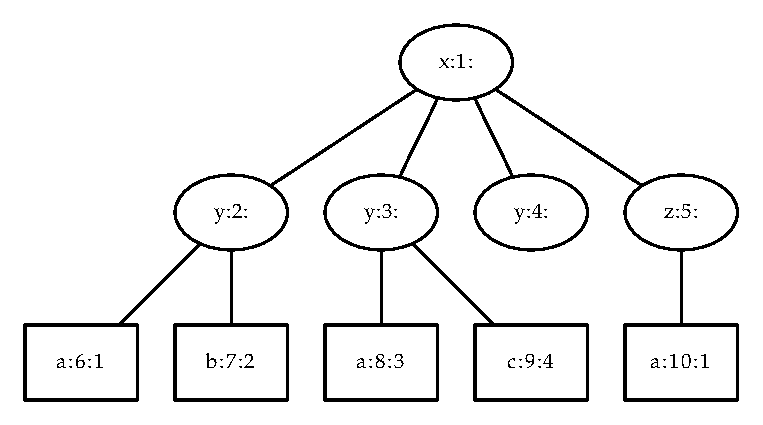
\includegraphics[width=.45\textwidth]{images/definitions/xml-tree}}
    \subfigure[Attribute Mappings]{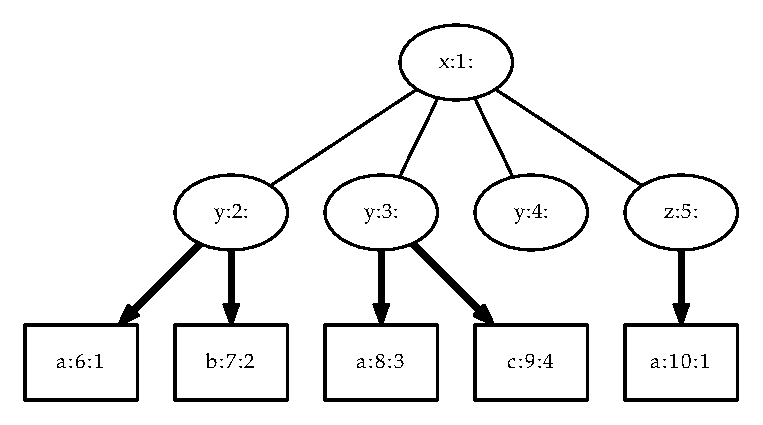
\includegraphics[width=.45\textwidth]{images/definitions/xml-tree-ams}}
\end{figure}

Furthermore, we denote $\mathcal{I}$ the set of all ids and $\mathcal{V}$ the set of all values in the document. We will need two more definitions from the article.

\begin{define}[Node equality]
	Nodes $v_1$ and $v_2$ are \textit{node equal}, written $v_1 =_n v_2$ iff $id(v_1) = id(v_2)$.
\end{define}

\begin{define}[Value equality]
	Nodes $v_1$ and $v_2$ are \textit{value equal}, written $v_1 =_v v_2$ iff $value(v_1) = value(v_2)$.
\end{define}

\section{\texttt{ID}, \texttt{IDREF}, \texttt{IDREFS} Attributes}
\label{section-definitions-id-attributes}

According to \cite{Bray:08:EML}, an XML attribute may have the type \texttt{ID}, \texttt{IDREF} or \texttt{IDREFS} (among others). The following constraints are related to these types.

\begin{quote}
\textbf{Validity constraint: \texttt{ID}}

Values of type \texttt{ID} \textsc{must} match the Name production. A name \textsc{must not} appear more than once in an XML document as a value of this type; i.e., \texttt{ID} values \textsc{must} uniquely identify the elements which bear them.

\textbf{Validity constraint: One \texttt{ID} per Element Type}

An element type \textsc{must not} have more than one \texttt{ID} attribute specified.

\textbf{Validity constraint: \texttt{ID} Attribute Default}

An \texttt{ID} attribute \textsc{must} have a declared default of \texttt{\#IMPLIED}\footnote{\texttt{\#IMPLIED} means that the attribute has a specified default value.} or \texttt{\#REQUIRED}\footnote{\texttt{\#REQUIRED} means that the attribute cannot be empty.}.

\textbf{Validity constraint: \texttt{IDREF}}

Values of type \texttt{IDREF} \textsc{must} match the Name production, and values of type \texttt{IDREFS} \textsc{must} match Names; each Name \textsc{must} match the value of an \texttt{ID} attribute on some element in the XML document; i.e. \texttt{IDREF} values \textsc{must} match the value of some \texttt{ID} attribute.
\end{quote}

\section{Attribute Mappings}
\label{section-definitions-ams}

Now we return to \cite{fidax} to define the notion of an \textit{attribute mapping} (or AM for short). \nomenclature{AM}{Attribute Mapping}
We will use a different definition (without introducing keys from \cite{keX}) that will however give us the same result.

\begin{define}[$\Sigma^E$, $\Sigma^A$, $\Sigma$]
	$\Sigma^E$ is the set of all element labels, $\Sigma^A$ is the set of all attribute labels. $\Sigma = \Sigma^E \cup \Sigma^A$ is their union and effectively the set of all labels in the document.
\end{define}

\begin{define}[Attribute mapping]
	For $x \in \Sigma^E$ and $y \in \Sigma^A$ we define the \textit{attribute mapping} of y over x, denoted $M_{x}^{y}$, the $\mathcal{I} \times \mathcal{I}$ relation defined by
	\[M_{x}^{y} = \{ (z,w): label(z) = x, label(w) = y, parent(w) = z \}.\]
\end{define}

Thus the relation $M_{x}^{y}$ contains edges in the XML tree connecting element nodes labeled $x$ and attribute nodes labeled $y$.

We can use projection to retrieve all the unique \textit{ids} of either elements or attributes from the relation, with notation $\pi_E(M_{x}^{y})$ and $\pi_A(M_{x}^{y})$.

\begin{define}[Type of the attribute mapping]
	Attribute mapping $M_{x}^{y}$ is of the \textit{type} $\tau(M_{x}^{y}) = x$.
\end{define}

\paragraph{Example}
The XML tree from Figure \ref{image-definitions-example-xml-tree}(b) has the following non-empty AMs drawn in bold lines: $M_{y}^{a} = \{(2,6), (3,8)\}$, $M_{y}^{b} = \{(2,7)\}$, $M_{y}^{c} = \{(3,9)\}$ and $M_{z}^{a} = \{(5,10)\}$.

The following example equations hold.
\begin{eqnarray*}
\pi_E(M_{y}^{a}) & = & \{2, 3\} \\
\pi_A(M_{z}^{a}) & = & \{10\} \\
\tau(M_{y}^{c}) & = & y
\end{eqnarray*}

\begin{define}[Image of the attribute mapping]
	\textit{Image} $\iota$ of the attribute mapping $M_{x}^{y}$ is defined as $\iota(M_{x}^{y}) = \{z: z = value(w), w \in \pi_A(M_{x}^{y})\}$.
\end{define}

So the image of an AM is a set of all the values of all the attribute nodes contained in the mapping.

\paragraph{Example}
Again referring to the XML tree from Figure \ref{image-definitions-example-xml-tree}, we get the following AM images.
\begin{eqnarray*}
\iota(M_{y}^{a}) & = & \{1, 3\} \\
\iota(M_{y}^{b}) & = & \{2\} \\
\iota(M_{y}^{c}) & = & \{4\} \\
\iota(M_{z}^{a}) & = & \{1\} \\
\end{eqnarray*}

\paragraph{Attribute Mapping Model}
An attribute mapping model is a data structure containing the information about all the AMs in a document, together with their images. We shall use this notion later in experimental part of this work.

\begin{define}[$name()$]
	Given an attribute mapping $m = M_{x}^{y}$, $name(m)$ shall be defined as the string $x-y$.
\end{define}

\section{ID Set}
\label{section-definitions-id-set}

Based on the requirements for an \texttt{ID} attribute from Section \ref{section-definitions-id-attributes} we will define ID set with the help of the following definition.

\begin{define}[Candidate attribute mapping]
An attribute mapping $m$ is a~\textit{candidate attribute mapping} if it is an injective function, that is,
\[|m| = |\pi_E(m)| = |\pi_A(m)| = |\iota(m)|.\]
\end{define}

\paragraph{Example}
In our example all the attribute mappings are candidate AMs.

Now we can proceed to define an ID set.

\begin{define}[ID set]
A set of candidate attribute mappings $I = \{m_1, \ldots m_n\}$ is an \textit{ID set} iff
\[\bigcap_{m_i \in I} \tau(m_i) = \emptyset \wedge \bigcap_{m_i \in I} \iota(m_i) = \emptyset.\]
\end{define}

That is, an ID set has images without repeating values and all the types are unique (an element cannot have more than one \texttt{ID} attribute).

\paragraph{Example}
Returning to our example, the following are all the possible ID sets: $\{ M_{y}^{a} \}, \{ M_{y}^{b} \}, \{ M_{y}^{b}, M_{z}^{a} \}, \{ M_{y}^{c} \}, \{ M_{y}^{c}, M_{z}^{a} \}$. Note that once we select an AM of type $y$ we can never add any other with the same type. Note also that $\{ M_{y}^{c}, M_{z}^{a} \}$ is not an ID set, because $\iota(M_{y}^{c}) \cap \iota(M_{z}^{a}) \neq \emptyset$.

\subsection*{\texttt{IDREF} and \texttt{IDREFS} Condition}

Given an ID set $I$, the requirements from Section \ref{section-definitions-id-attributes} give us the following condition for an attribute mapping $m$ to be marked \texttt{IDREF}:
\[\iota(m) \subseteq \bigcup_{m_i \in I} \iota(m_i).\]
Furthermore, if $m$ contains multivalued attributes, it is to be marked \texttt{IDREFS}.

\section{Attribute Mapping Weight}
\label{section-definitions-weight}

This definition of weight for AMs or AM sets comes from \cite{fidax} again. Let $M = \{m_1, \dots m_i\}$ be the set of all non-empty AMs in the document.

\subsection{Support}

\begin{define}[Support]
\textit{Support} of an attribute mapping $m$ is defined as follows:
\[\phi(m) = \frac{|m|}{\sum_{p \in M}|p|}.\]
\end{define}

\begin{quote}
The support of attribute mapping $M_x^y$ is the fraction of edges in~the~XML tree that connect $x$ elements to $y$ attributes.
\end{quote}

\paragraph{Example}
Support of $M_{y}^{a}$ in our example is $2 / (2+1+1+1) = 0.4$. Support of~every other mapping is $1 / (2+1+1+1) = 0.2$.\\

\subsection{Coverage}

\begin{define}[Coverage]
\textit{Coverage} of an attribute mapping $m$ is defined as follows:
\[\chi(m) = \left( \sum_{p \in M, p \neq m} |\iota(m) \cap \iota(p)| \right) / \sum_{p \in M} |\iota(p)|.\]
\end{define}

\begin{quote}
The coverage of an attribute mapping measures how much of the image of that mapping occurs elsewhere, as a fraction of all mappings images in the document.
\end{quote}

\paragraph{Example}
Coverage of $M_{y}^{a}$ in our example is $(0+0+1) / (2+1+1+1) = 0.2$. Coverage of $M_{z}^{a}$ is $0.2$ as well, all the other mappings have coverage $0$.
\\

\textit{Weight} of an attribute mapping is then defined as a linear combination of its support and coverage.

\begin{define}[Weight]
For $\alpha, \beta \geq 0$ as relative priorities of support and coverage we define the AM \textit{weight} as follows:
\[weight(m) = \alpha . \phi(m) + \beta . \chi(m).\]
For a set of AMs (which may or may not be an ID set) $S = \{m_1, \ldots m_i\}$ we define the weight of this set as the sum of the weights of its AMs:
\[weight(S) = \sum_{m \in S} weight(m).\]
\end{define}

Note that this definition of weight is quite arbitrary and all the algorithms mentioned later could easily work with AM weight defined in any other way, even for example defined interactively by the user.

\section{Independent Set}
\label{section-definitions-is}

\nomenclature{IS}{Independent Set}

We shall need the notion of an indepentent set (IS) of vertices in a graph and its weighted variant.

\begin{define}[Independent set]
Given an undirected graph $G = (V, E)$, a set of vertices $I \subseteq V$ is an \textit{independent set}, iff
\[\forall v_1, v_2 \in I, v_1 \neq v_2: (v_1, v_2) \notin E.\]
\end{define}

\begin{define}[Maximum weighted independent set]
Given an undirected graph $G = (V, E)$ and a weight function $w: V \rightarrow \mathbb{R}$, an independent set $I_{max}$ is the \textit{maximum weighted independent set}, iff the following is satisfied:
\[\forall I' \subseteq V, I' \text{is an independent set}: \sum_{v \in I'} w(v) \leqslant \sum_{v \in I_{max}} w(v).\]
\end{define}

It is well known that finding the maximum weighted IS is an NP-hard optimization problem, \cite{JM1986425}.

\section{Linear Programming}

The problem of \textit{linear programming} is optimization of a~linear function under a~set of linear constraints. The formulation is usually called a~\textit{linear program}. 

It can be written in the following form:

\begin{eqnarray*}
\max_{x} z & = & \mathbf{c}^{\mathrm{T}}\mathbf{x} \\
s.t.\, A\mathbf{x} & \leqslant & \mathbf{b} \\
\mathbf{x} & \geqslant & 0 \\
\end{eqnarray*}
\[
\mathbf{x} =
\begin{bmatrix}
x_1 \\
x_2 \\
\ldots \\
x_n \\
\end{bmatrix},
\mathbf{c} = 
\begin{bmatrix}
c_1 \\
c_2 \\
\ldots \\
c_n \\
\end{bmatrix},
\mathbf{b} =
\begin{bmatrix}
b_1 \\
b_2 \\
\ldots \\
b_m \\
\end{bmatrix},
\]

where a minimization version is possible, too.

Where $\mathbf{x}$ is the vector of variables (to be found by the optimization), $\mathbf{b}$ is the vector and $A$ its accompanying matrix of constraints and $\mathbf{c}$ is the vector of coefficients for the objective function. $\mathbf{x}$ and $\mathbf{c}$ have length $n$, $\mathbf{b}$ has length $m$ and $A$ has dimensions $m \times n$. Furthermore, \[\max_{x} f(x)\] means maximize the value of $f(x)$ by changing the value of $x$.\\

Another way to write this formulation is this:

\begin{eqnarray*}
\max_{x} z = \sum_{i=1}^{n} c_i x_i \\
s.t. & \\
	   a_{11}x_{1} + a_{12}x_{2} + \ldots + a_{1n}x_{n} & \leqslant & b_{1} \\
	   a_{21}x_{1} + a_{22}x_{2} + \ldots + a_{2n}x_{n} & \leqslant & b_{2} \\
	   \ldots \\
	   a_{m1}x_{1} + a_{m2}x_{2} + \ldots + a_{mn}x_{n} & \leqslant & b_{m} \\
	   x_i \geqslant 0, i = 1, \ldots n \\
\end{eqnarray*}

Solving a linear program is usually possible in polynomial time using the~\textit{simplex algorithm} described for example in \cite{dantzig1998linear}.

\section{Mixed Integer Problem}

\nomenclature{MIP}{Mixed Integer Problem}

\begin{define}[Mixed integer problem]
	MIP, or \textit{mixed integer problem}, is an~instance of~linear programming in~which some or~all variables are limited to~integral or~boolean (0, 1) values.
\end{define}

Solving MIP in general is $\NP$-hard.

\chapter{Related Work}
\label{chapter-research}

According to the article \cite[Chapter~4]{fidax}, the problem of finding an ID set with weight more than some $K$ ($K$-\textsc{IDSet}) is in NP. Furthermore, the independent set (IS) problem can be reduced to $K$-\textsc{IDSet}, meaning $K$-\textsc{IDSet} is NP-hard and thus NP-complete. The transformation from IS problem formulation to~$K$-\textsc{IDSet} problem formulation is as follows.

\begin{quote}
Let $G = (V, E)$ be a simple connected graph with vertex set $V = \{v_1, \ldots, v_n\}$, and edge set $E = \{e_1, \ldots, e_m\}$. We define the attribute mappings as follows. Let $ \mathcal{I} = V \cup E$, and define $value(x) = x, x \in \mathcal{I}$. For each vertex $v_i \in V$, we create a mapping $m_i = \{(v_i, e_j): e_j \in E \,\text{is incident on}\, v_i \}$, and define $\tau(m_i) = v_i$; let $C = \{m_1, \ldots, m_n\}$ be set of all such mappings. It is clear that G has an independent set of size $K$ iff $C$ has an ID set of size $K$. Also, $C$ can be constructed in time polynomial on $n+m$.
\end{quote}

The article continues by proving that finding the maximum weighted IS can be reduced to the problem of finding an ID set with maximum weight (\textsc{Max-IDSet}). This again means that \textsc{Max-IDSet} is NP-complete and, furthermore, unless $\P = \NP$, \textsc{Max-IDSet} has no constant factor approximation algorithm.

The difference in transformation from maximum weighted IS to \textsc{Max-IDSet} is as follows.

\begin{quote}
[...] with the added restriction that $w(m_i) = w(v_i), v_i \in V$.
\end{quote}

Note that the transformation works in both ways: it is equivalently possible to create a maximum weighted IS instance for a given \textsc{Max-IDSet} instance.

The article further suggests a heuristic approach described in Section \ref{section-mip-fidax}, which was incorporated into the framework proposed by this work.

To the best of our knowledge, there are no other articles dealing with this problem.\\

\section{Finding XML Keys}

XML keys are a structure somewhat similar to \texttt{ID} attributes, but with a much larger expressive strength. They have been introduced in \cite{keX} and implemented in XML Schema\footnote{\url{http://www.w3.org/TR/xmlschema11-1/\#Identity-constraint\_Definition\_details}}.

Fajt in \cite{fajt} summarizes several algorithms to help find XML keys in existing data, namely \textit{Gordian}, \textit{XML Primary Keys}, \textit{SPIDER} and \textit{DBA Companion}. Except for \textit{XML Primary Keys}, they all are originally purposed to find keys in~relational databases. We will describe them shortly.

\subsubsection{\textit{Gordian}}

This algorithm from \cite{fajt-41} extracts composite primary keys (PKs) from relational databases.

\begin{quote}
The idea behind is an observation that a projection of entities corresponds to a key if each counted aggregation for a projection is equal to 1. Thus, this method searches for all possible projections of a dataset while computing aggregations on the projected part of the set of entities.
\end{quote}

This is achieved by constructing a prefix tree from the tuples in the original relation, which is then pruned and traversed depth-first to find non-key attributes from which the primary keys are inferred. This algorithm still has to~be~adapted to~search for PKs in XML data.

\subsubsection{\textit{XML Primary Keys}}

This is an algorithm from \cite{fajt-39} capable of finding simple keys and foreign keys directly in XML data. This is achieved by building a prefix tree containing all the XML nodes and then evaluating every path in it as a candidate key using metrics called \textit{support} and \textit{confidence}. To find more complex keys, the algorithm iteratively constructs candidate keys from simpler ones and evaluates them.\\

The following two algorithms deal with \textit{inclusion dependencies} (INDs), described for example in \cite{fajt-12}.

\subsubsection{\textit{SPIDER}}

The core of this algorithm from \cite{fajt-51, fajt-53} is the following.

\begin{quote}
The process consists of two steps - sets of values are sorted during the first one and then all the candidates are analyzed in parallel. The core of the method is utilizing the data structure called min-heap which synchronizes the processing of all values of all attributes.
\end{quote}

It is~possible to~use a~number of~heuristic pruning strategies to~keep the~min-heap in~a~reasonable size. This algorithm performs very well for PKs in~relational databases, however, it~still has to~be~adapted for~XML keys.

\subsubsection{\textit{DBA Companion}}

Like \textit{SPIDER}, this method from \cite{fajt-53} is able to find all the~INDs in~the~da\-ta\-base in~just one pass. However, it~uses a~different data structure (basically a~binary relation between the~attributes and~their corresponding values) and~considers data types. Composite INDs are~found using the~simple ones and~pruning the~search space. According to~the~authors of~\textit{SPIDER}, \textit{DBA Companion} is~far inferior in~performance. This algorithm has yet to~be~adapted to~search for XML keys, too.

\subsubsection{Fajt's Approach - \textit{KeyMiner}}

Fajt introduces a new algorithm based on \textit{Gordian} and \textit{SPIDER} to look for primary and foreign keys in XML data. First, relations have to be extracted from the original XML document. Then all the primary keys are found using a modified \textit{Gordian} algorithm which can find absolute as well as relative PKs. Finally, \textit{SPIDER} is used to compute the foreign keys from the PKs found in the previous step.

\subsection{Relation to \texttt{ID} Attributes}

XML keys found this or any other way can under some circumstances (when they are simple enough) be translated to an equivalent \texttt{ID} attribute definition. The process is described in \cite[Ch.\ 9, s.\ 3]{vlist2002xml}. This opens a new line of possible research: finding XML keys using an algorithm modified to look only for \textit{useful} keys and then converting them to \texttt{ID} attributes.\\ 

However, in our work we find \texttt{ID} attributes directly. And even though we can always convert them to XML keys by the process mentioned above, we are unable to find more complex keys this way.\\

\section{Maximum Weighted IS}

Maximum weigthed IS is a well researched topic with a lot of known direct or approximation algorithms, see e.g. \cite{JM1986425} or \cite{Fomin:2009:MCA:1552285.1552286}. According to for example \cite{Paschos:1997:SAO:254180.254190}, the best known approximation algorithm for weighted IS to-date achieves an approximation ratio of $3(\Delta + 2)$, where $\Delta$ is the maximum degree of a vertex in the IS graph. This article lists several algorithms similar to those we introduce in the following chapters.\\

\chapter{MIP Approach}
\label{chapter-mip}

In this chapter we introduce a new approach to finding maximum ID sets. First, we transform the problem formulation to maximum weighted IS problem formulation. Then we transform this into a MIP formulation, and demonstrate how this can be solved using a solver such as GLPK. \nomenclature{GLPK}{GNU Linear Programming Kit}
We will continue by applying heuristical approaches to improve the performance of the process.

\section{ID Set to IS Formulation}

Given $C = \{m_1, \ldots, m_n\}$ a set of all AMs in a document, we construct a graph $G = (V,E)$ as follows. For each AM $m_i \in C$ we create a vertex $v_{name(m_i)}$. Two vertices $v_{name(m_i)}$ and $v_{name(m_j)}$ shall be connected by an edge iff they cannot share the same ID set, either because they have the same type ($\tau(m_i) = \tau(m_j)$), or their images intersect ($\iota(m_i) \cap \iota(m_j) \neq \emptyset$). Weight of a vertex $v_{name(m_i)}$ is the weight of the attribute mapping: $w(v_{name(m_i)}) = weight(m_i)$.

Now finding the maximum weighted IS in $G$ finds the maximum (optimal) ID set in the original document.

\section{IS to MIP Formulation}

Given a graph $G = (V,E)$ with a weight function $w: V \rightarrow \mathbb{R}$, we introduce a binary variable $x_i$ for each vertex $v_i \in V$ and an inequality constraint $x_i + x_j \leq 1$ for each edge $e = (v_i, v_j) \in E$. Furthermore we introduce an objective function in form $\sum_{x_i} x_i w(v_i)$.

It is obvious that the objective function and all the constraints consitute a MIP instance, and that solving it finds the maximum weigthed IS in $G$.

\section{Finding ID Sets With GLPK}

By chaining these two translations we can create a MIP formulation for a given set of AMs from a document. Solving this MIP instance will give us the optimal ID set for this document.

GLPK \cite{glpk} is a multi-platform, multi-purpose solver well suited for this task. It uses the Simplex method to solve LP problems and \textit{Branch \& Bound} (see \cite{land60a} for details) for MIP. An advantage of using \textit{Branch \& Bound} is that while traversing the \textit{search tree} it finds intermittent, sub-optimal solutions. It is thus possible to limit the total search time and instead of the optimum take the best solution found so far.\\

We will now demonstrate the full process of finding the optimal ID set of an example XML file using GLPK.

\subsection{Example}

Consider again our XML file fragment.

\begin{verbatim}
<x>
  <y a="1" b="2"/>
  <y a="3" c="4"/>
  <y/>
  <z a="1"/>
</x>
\end{verbatim}

Recall that attribute mappings in this example are $C = \{M_{y}^{a}, M_{y}^{b}, M_{y}^{c}, M_{z}^{a}\}$. Corresponding vertices in the IS formulation will be $V = \{v_{y-a}, v_{y-b}, v_{y-c}, v_{z-a}\}$. Edges in the IS formulation will be the following.

\begin{eqnarray*}
(v_{y-a},v_{y-b}) \\
(v_{y-a},v_{y-c}) \\
(v_{y-b},v_{y-c}) \\
(v_{y-a},v_{z-a}) \\
\end{eqnarray*}

First three edges are due to the type collision ($y$), the last one is due to $\iota(M_{y}^{a}) \cap \iota(M_{z}^{a}) = \{1\}$. The graph $G$ constructed in this way is in Figure \ref{image-mip-is-graph}.

\begin{figure}
  \caption{IS Representation Graph}
  \label{image-mip-is-graph}
  \centering
	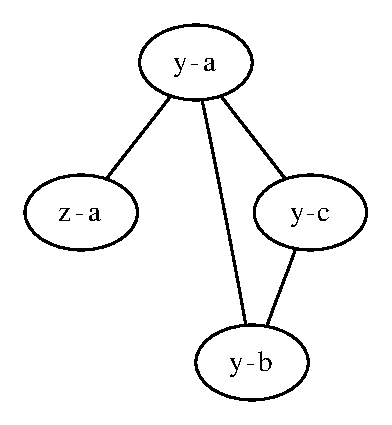
\includegraphics[width=.25\textwidth]{images/is-representation}
\end{figure}

The next step is the MIP formulation. We do not need to translate from the IS formulation, as the translation from ID set formulation is straightforward, too. For each AM $m$ there will be one binary variable $x_{name(m)}$. Objective function coefficients in vector $\mathbf{c}$ will be weights of respective mappings. For each pair of AMs $m_1, m_2$ that cannot share the same ID set there shall be a row in matrix $A$ representing the inequality $x_{name(m_1)} + x_{name(m_2)} \leqslant 1$. $\mathbf{b}$ will be a vector of ones with corresponding length.

\[
\mathbf{x} =
\begin{bmatrix}
x_{y-a} \\
x_{y-b} \\
x_{y-c} \\
x_{z-a} \\
\end{bmatrix},
\mathbf{c} = 
\begin{bmatrix}
weight(M_{y}^{a}) \\
weight(M_{y}^{b}) \\
weight(M_{y}^{c}) \\
weight(M_{z}^{a}) \\
\end{bmatrix} =
\begin{bmatrix}
0.2 \\
0.2 \\
0.6 \\
0.4 \\
\end{bmatrix},
\mathbf{b} =
\begin{bmatrix}
1 \\
1 \\
1 \\
1 \\
\end{bmatrix},
A =
\begin{pmatrix}
0 & 1 & 1 & 0 \\
1 & 0 & 1 & 0 \\
1 & 1 & 0 & 0 \\
1 & 0 & 0 & 1 \\
\end{pmatrix}
\]

The problem now is, recall, to solve the following.

\begin{eqnarray*}
\max_{x} z & = & \mathbf{c}^{\mathrm{T}}\mathbf{x} \\
s.t.\, A\mathbf{x} & \leqslant & \mathbf{b} \\
\end{eqnarray*}

In GLPK \textit{MathProg} language, this translates to the following formulation. % TODO cite mathprog

\begin{scriptsize}
\begin{verbatim}
set AMs;
param Weight {i in AMs};
var x {i in AMs} binary;
maximize z: sum {i in AMs} x[i] * Weight[i];
s.t. c1: x['y-a'] + x['y-b'] <= 1;
s.t. c2: x['y-a'] + x['y-c'] <= 1;
s.t. c3: x['y-b'] + x['y-c'] <= 1;
s.t. c4: x['y-a'] + x['z-a'] <= 1;
data;
set AMs := y-a y-b y-c z-a;
param Weight :=
y-a 0.6
y-b 0.2
y-c 0.2
z-a 0.4;
end;
\end{verbatim}
\end{scriptsize}

We can use this as an input for the GLPK solver, and we get the solution.

\begin{scriptsize}
\begin{verbatim}
...
Problem:    glpk_input
Rows:       5
Columns:    4 (4 integer, 4 binary)
Non-zeros:  12
Status:     INTEGER OPTIMAL
Objective:  z = 0.6 (MAXimum)

...

   No. Column name       Activity     Lower bound   Upper bound
------ ------------    ------------- ------------- -------------
     1 x[y-a]       *              1             0             1 
     2 x[y-b]       *              0             0             1 
     3 x[y-c]       *              0             0             1 
     4 x[z-a]       *              0             0             1 

...
\end{verbatim}
\end{scriptsize}

This output tells us that the solution is $x_{y-a} = 1$, $x_{y-b} = 0$, $x_{y-c} = 0$ and $x_{z-a} = 0$. This means that the optimal ID set with maximum weight contains only the $M_{y}^{a}$ attribute mapping.\\

It is obvious that this approach works and for any possible input we can let GLPK find the optimal solution. However, sometimes it takes too long to find the optimum (see e.g. Section \ref{section-glpk-comparison}), we should try to improve this process.

\section{Heuristics}

TODO what is heuristics (link wise books), what is metaheuristics (we will be using them)

TODO mention things like Taboo search and Genetic Algorithms (we can emulate them with Crossover/Mutation) (we won't be using them)

TODO we will be working with heuristics striving to do the following: input is a list of AMs, they have their weight, we try to find a non-conflicting subset which maximizes the weight

TODO we will be using a pool - what is a pool

\begin{figure}
  \caption{Metaheuristic schema}
  \label{image-metaheuristic}
  \centering
    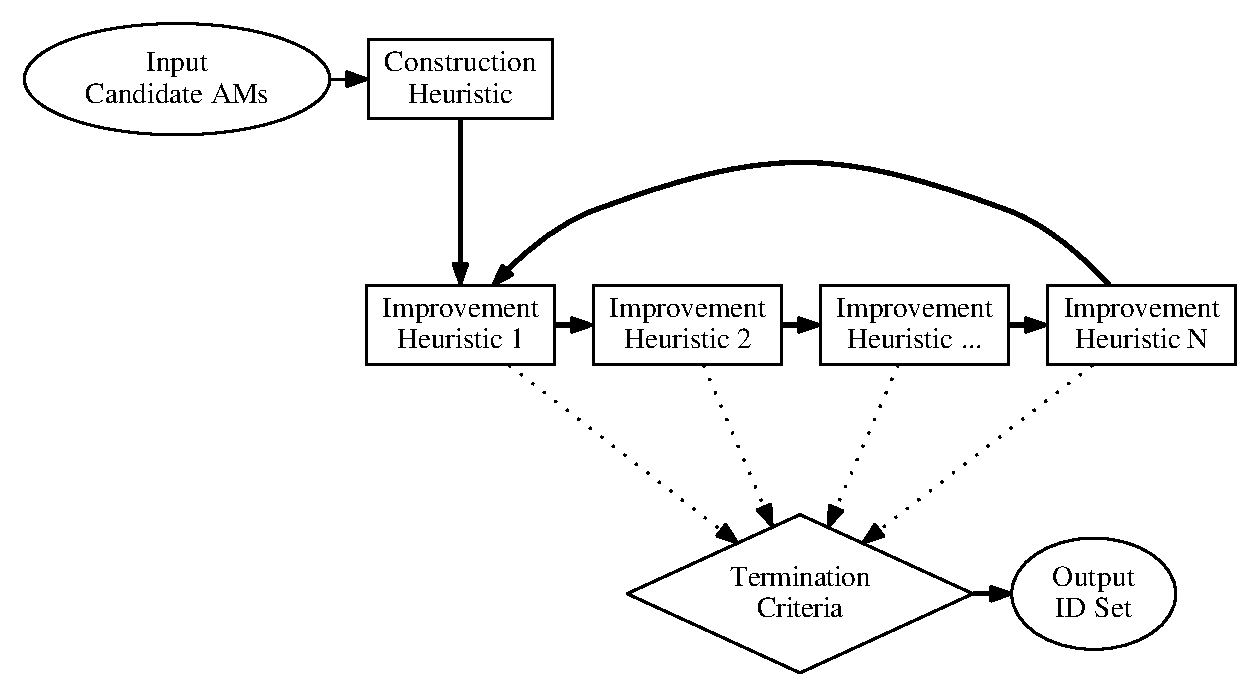
\includegraphics[width=\textwidth]{images/metaheuristic}
\end{figure}

\subsection{Constructions Heuristics}
% TODO can I format things in nomenclature?
\nomenclature{CH}{Construction Heuristic} %TODO decide on how to format CH/IH

TODO construction heuristics are heus that provide us with at least some solution.

\subsubsection{\heu{FIDAX}}
\label{section-mip-fidax}

It should be obvious by now that the algorithm described in \cite{fidax} (we shall call it \heu{FIDAX} from now on) can trivially be used as a construction heuristic that will give us one feasible solution.

The pseudocode of this CH (taken from the original article with trivial modifications without changing the logic) is in Listing \ref{listing-ch-fidax}.

\begin{algorithm}
\caption{\heu{FIDAX} CH}
\label{listing-ch-fidax}
\begin{algorithmic}
\REQUIRE $C$ list of candidate AMs
\ENSURE a feasible solution
\STATE $C' \gets C$ sorted by decreasing size
\STATE Compute the weight $w(m)$ of each $m$ in $C$
\FORALL{$t$ in $\Sigma^E$}
  \STATE Let $m$ be a \textbf{highest-weight} mapping of type $t$ in $C'$
  \STATE Remove from $C'$ all mappings of type $t$ except $m$
\ENDFOR
\FORALL{$m$ in $C'$}
  \STATE $S \gets$ all mappings in $C$ whose images intersect $\iota(m)$
  \IF{$w(m) > \sum_{p \in S} w(p)$}
    \STATE remove all $p \in S$ from $C'$
  \ELSE
    \STATE remove $m$ from $C'$
  \ENDIF
\ENDFOR
\RETURN $C'$
\end{algorithmic}
\end{algorithm}

\subsubsection{\heu{Random}}
\label{heu-ch-random}

One of the most natural heuristics when dealing with the IS problem can be described as follows: select from candidate AMs at random, if possible (addition would not violate the ID set condition) add them to the solution. This is obviously a hungry heuristic. %TODO have I defined ID set condition yet??

The advantages of this trivial heuristic are simplicity, speed and ease with which it can create a pool of variable solutions, almost for free. As we will see later in the experiments (Section \ref{section-experiments-random-fuzzy-fidax}), it performs surprisingly well.

See the Listing \ref{listing-ch-random} for its pseudocode.

\begin{algorithm}
\caption{\heu{Random} CH}
\label{listing-ch-random}
\begin{algorithmic}
\REQUIRE $N$ required size of pool
\REQUIRE $C$ list of candidate AMs
\ENSURE pool of $N$ feasible solutions
\STATE $r \gets $ empty pool
\FOR{$i = 1 \to N$}
  \STATE \COMMENT{create 1 solution}
  \STATE $s \gets $ empty solution
  \WHILE{$s$ is a feasible ID set}
    \STATE $a \gets $ pick at random from $C \backslash S$
    \STATE $s \gets s \cup a$
  \ENDWHILE
  \STATE $r \gets r \cup s$
\ENDFOR
\RETURN $r$
\end{algorithmic}
\end{algorithm}

\subsubsection{\heu{Fuzzy}}
\label{heu-ch-fuzzy}

\heu{Fuzzy} is an improvement over the \heu{Random} CH: it picks the next AM to try to add based on \textit{weighted} instead of uniform random. The weight used here is the usual weight of an AM as defined in TODO. Because of the randomness involved in the choice, we can again easily create a pool of solutions this way.

Again, this is a hungry heuristic, the Listing \ref{listing-ch-fuzzy} contains its pseudocode.

% TODO od I need to specify which are my own idea? I guess so, I should link any heu that is not mine. But do I need to stress that for example Fuzzy is mine?

\begin{algorithm}
\caption{\heu{Fuzzy} CH}
\label{listing-ch-fuzzy}
\begin{algorithmic}
\REQUIRE $N$ required size of pool
\REQUIRE $C$ list of candidate AMs
\ENSURE pool of $N$ feasible solutions
\STATE $r \gets $ empty pool
\FOR{$i = 1 \to N$}
  \STATE \COMMENT{create 1 solution}
  \STATE $s \gets $ empty solution
  \STATE $C' \gets C$

  \WHILE{$C' $ not empty}
    \STATE $a \gets $ pick at weighted random from $C'$
    \IF{$s \cup a$ is a feasible ID set}
      \STATE $s \gets s \cup a$
      \STATE $C' \gets C' \backslash a$
    \ENDIF
    \FORALL{$c \in C'$}
      \IF{$s \cup c $ is \textbf{not} a feasible ID set}
        \STATE \COMMENT {if $c$ cannot be possibly added anymore}
        \STATE $C' \gets C' \backslash c$
      \ENDIF
    \ENDFOR
  \ENDWHILE

  \STATE $r \gets r + s$
\ENDFOR
\RETURN $r$
\end{algorithmic}
\end{algorithm}

\subsubsection{\heu{Incremental}}

This trivial heuristics sorts all candidate AMs by their decreasing weights (Section \ref{section-definitions-weight}) and then tries to iteratively add them to solution, if possible. This way it can create only one solution, and again, this is a hungry heuristic.

See listing \ref{listing-ch-incremental}.

\begin{algorithm}
\caption{\heu{Incremental} CH}
\label{listing-ch-incremental}
\begin{algorithmic}
\REQUIRE $C$ list of candidate AMs
\ENSURE a feasible solution
\STATE $C' \gets $ sort $C$ by decreasing weight
\STATE $s \gets $ empty solution
\FORALL{$c \in C'$}
  \IF{$s \cup c$ is a feasible ID set}
    \STATE $s \gets s + c$
  \ENDIF
\ENDFOR
\RETURN $s$
\end{algorithmic}
\end{algorithm}

\subsubsection{\heu{Removal}}

This is basically a reversal of the idea from the \heu{Incremental} heuristic - start with a solution containing all the candidate AMs. This probably does not satisfy the ID set condition. Therefore, order them by increasing size and start removing them from the solution, until it satisfies the ID set condition. Again, this is a hungry heuristic returning only one solution.

See listing \ref{listing-ch-removal}.

\begin{algorithm}
\caption{\heu{Removal} CH}
\label{listing-ch-removal}
\begin{algorithmic}
\REQUIRE $C$ list of candidate AMs
\ENSURE a feasible solution
\STATE $C' \gets $ sort $C$ by increasing weight
\STATE $s \gets C'$
\FORALL{$c \in s$}
  \IF{$s$ is a feasible ID set}
    \RETURN $s$
  \ENDIF
  \STATE $s \gets s \backslash c$
\ENDFOR
\end{algorithmic}
\end{algorithm}

\subsubsection{Truncated Branch \& Bound}

This CH will be called \heu{Glpk} from now on, for it is basically a time-constrained run of GLPK.

TODO if we limit GLPK's runtime, we get this

TODO we shuffle AMs - we get different runs - pool is possible

\subsection{Improvement Heuristics}
\label{section-mip-ihs}

\nomenclature{IH}{Improvement Heuristic}

TODO what they are, that they need a pool sometimes, their input and output is a pool, ...

TODO mention intensification, diversification

TODO mention that combination of \heu{Crossover}, \heu{Mutation} and \heu{RemoveWorst} is a sort of genetic algorithm

\subsubsection{\heu{Identity}}

This ultimately trivial improvement heuristics does nothing. It simply returns the feasible pool unchanged. For the sake of completeness, see its listing \ref{listing-ih-identity}.

\begin{algorithm}
\caption{\heu{Identity} IH}
\label{listing-ih-identity}
\begin{algorithmic}
\REQUIRE $FP$ pool of feasible solutions
\ENSURE the same pool of feasible solutions
\RETURN $FP$
\end{algorithmic}
\end{algorithm}

\subsubsection{\heu{Remove Worst}}

This trivial IH tries to improve the solution pool by removing the worst solution (i.e. the one with the lowest quality). This might be interesting in cooperation with other improvement heuristics that increase the solution pool size, to keep it from growing by pruning inferior solutions.

See listing \ref{listing-ih-removeworst}.

\begin{algorithm}
\caption{\heu{Remove Worst} IH}
\label{listing-ih-removeworst}
\begin{algorithmic}
\REQUIRE $FP$ pool of feasible solutions
\ENSURE pool of feasible solutions
\STATE $s_{min} \gets $ solution with the lowest weight $\in FP$
\RETURN $FP \backslash s_{min}$
\end{algorithmic}
\end{algorithm}

\subsubsection{\heu{Random Remove}}

This is again a rather trivial IH, something which is usually referred to as a \textit{perturbation} function. % TODO link the notion
By removing a random subset of specified size from each solution in the pool, it provides variability needed to escape from local optima. % TODO make sure we have talked about local optima before

The number of AMs to remove from each solution is specified as ratio (from the interval $(0, 1)$) of the solution size. % TODO have we defined what a solution size is?
For example, \heu{Random Remove} with $ratio = 0.1$ would remove 1 random AM from a solution containing 10 AMs and 2 from a solution containing 17 AMs (due to rounding).

This heuristic returns a pool of solutions of the same size as it got on its input.

See listing \ref{listing-ih-randomremove}.

\begin{algorithm}
\caption{\heu{Random Remove} IH}
\label{listing-ih-randomremove}
\begin{algorithmic}
\REQUIRE $FP$ pool of feasible solutions
\REQUIRE $k \in (0,1)$ ratio of AMs to remove from each $s \in FP$
\ENSURE pool of feasible solutions
\FORALL{$s \in FP$}
  \STATE $K \gets k * |s|$
  \STATE remove $K$ random AMs from $s$
\ENDFOR
\RETURN $FP$
\end{algorithmic}
\end{algorithm}

\subsubsection{\heu{Hungry}}

This simple improvement heuristic assumes that the solutions in the pool are not ``complete", i.e. there are AMs that could be added to them without violating the ID set condition.

\heu{Hungry} tries to improve each solution in the feasible pool in the following way. It orders all candidate AMs not present in the solution by decreasing weight. Afterwards, it iteratively tries to extend the solution with these AMs, taking care not to violate the ID set condition. The resulting solution (whether any AMs were added or not) is then returned to the pool. Listing \ref{listing-ih-hungry} captures this process.

\begin{algorithm}
\caption{\heu{Hungry} IH}
\label{listing-ih-hungry}
\begin{algorithmic}
\REQUIRE $FP$ pool of feasible solutions
\REQUIRE $C$ list of candidate AMs
\ENSURE pool of feasible solutions
\FORALL{$s \in FP$}
  \STATE \COMMENT {improve a single solution}
  \STATE $C' \gets C \backslash s$
  \STATE $C' \gets C'$ sorted by decreasing weight
  \FORALL{$c \in C'$}
    \IF{$s \cup c$ is a feasible ID set}
      \STATE $s \gets s \cup c$
    \ENDIF
  \ENDFOR
\ENDFOR
\RETURN $FP$
\end{algorithmic}
\end{algorithm}

\subsubsection{\heu{Mutation}}

TODO explain how this works and link wise books

TODO explain how this translates to GLPK input

For every AM $AM_F$ fixed to appear in the solution a following constraint is added to GLPK input:
\[s.t. f_{index}: x['name(AM_F)'] = 1;\]
$index$ is a unique integer to number all the constraints.

Additionaly, every other mapping $AM_i$ colliding with $AM_F$ ($\iff \iota(AM_F) \cap \iota(AM_i) \neq \emptyset$) will cause the following constraint to be added:
\[s.t. f_{index}: x['name(AM_i)'] = 0;\]
And the original constraint in form:
\[s.t. c_{index}: x['name(AM_F)'] + x['name(AM_i)'] <= 1;\]
will not be included.

See listing \ref{listing-ih-mutation}.

\begin{algorithm}
\caption{\heu{Mutation} IH}
\label{listing-ih-mutation}
\begin{algorithmic}
\REQUIRE $FP$ pool of feasible solutions
\REQUIRE $k$ ratio of AMs to fix
\ENSURE pool of feasible solutions
\STATE $incumbent \gets $ best solution in $FP$ \COMMENT {best = highest weight}
\STATE $K \gets k * |incumbent|$
\STATE fix $K$ random AMs from $incumbent$ in GLPK problem formulation
\STATE $improved \gets $ run GLPK
\RETURN $FP \cup improved$
\end{algorithmic}
\end{algorithm}

\subsubsection{\heu{Crossover}}

TODO explain how this works and link wise books

TODO explain how this translates to GLPK input - it's again simple fixing to 1, but we get the list of AMs in a different manner.

See listing \ref{listing-ih-crossover}.

\begin{algorithm}
\caption{\heu{Crossover} IH}
\label{listing-ih-crossover}
\begin{algorithmic}
\REQUIRE $FP$ pool of feasible solutions
\REQUIRE $k$ ratio of solutions to look for commonalities in
\ENSURE pool of feasible solutions
\STATE $K \gets k * |FP|$
\STATE $FP' \gets K$ random solutions $\in FP$
\STATE $am \gets$ AMs found in all solutions $\in FP'$
\STATE fix $am$ in GLPK problem formulation
\STATE $improved \gets $ run GLPK
\RETURN $FP \cup improved$
\end{algorithmic}
\end{algorithm}

\subsubsection{\heu{Local Branching}}

TODO explain how this works and link wise books

TODO explain how this translates to GLPK input

A new constrain describing the maximal allowed distance from the incumbent solution is added to GLPK input.

\[s.t. LB: sum\{i\ in\ INCUMBENT\} (1 - x[i]) + sum\{i\ in\ REMAINING\} x[i] \leq k;\]

Where $INCUMBENT$ is a set of names of AMs in the incumbent solution, $REMAINING$ is a set of all the AMs not included in the incumbent solution and $k$ is the requested maximal distance.

See listing \ref{listing-ih-localbranching}.

\begin{algorithm}
\caption{\heu{Local Branching} IH}
\label{listing-ih-localbranching}
\begin{algorithmic}
\REQUIRE $FP$ pool of feasible solutions
\REQUIRE $k$ ratio of total AM count to bound the Hamming distance to
\ENSURE pool of feasible solutions
\STATE $K \gets k * |$total AM count$|$
\STATE $incumbent \gets $ best solution in $FP$ \COMMENT {best = highest weight}
\STATE add max Hamming distance requirement to GLPK problem formulation
\STATE $improved \gets $ run GLPK
\RETURN $FP \cup improved$
\end{algorithmic}
\end{algorithm}

\section{IDREF}

Once an ID set is found, regardless of how exactly, it is easy to find the IDREF set, i.e. the attribute mappings that can be declared as IDREF. % TODO link FIDAX, they did it first.

First of all, from the set of all the attribute mappings in the model remove all the AMs contained in the ID set. This is because the specification % TODO link to the specific anchor in the page
does not allow an attribute to be ID and IDREF (IDREFS) at the same time. Let us denominate these mappings as \textit{IDREF candidates} (obviously different from \textit{candidate AMs}). % TODO link candidate AMs

Second, find the image of the ID set as the union of images of all the AMs in this ID set.

\[\iota(ID) = \bigcup_{am \in ID} \iota(am)\]

Now the IDREF set contains all the AMs whose images are a subset of the ID set image.

\[\iota(c) \subset \iota(ID) \Rightarrow c \in IDREF\]

This can be easily determined in a loop over the list of candidates. The process is captured in Listing \ref{listing-idref}.

\begin{algorithm}
\caption{IDREF Search}
\label{listing-idref}
\begin{algorithmic}
\REQUIRE $AMs$ list of all AMs
\REQUIRE $ID$ ID set as a list of AMs
\ENSURE $IDREF$ set as a list of AMs
\STATE $IDREF \gets \emptyset$
\STATE $candidates \gets AMs \backslash ID$
\STATE $\iota(ID) \gets \bigcup_{am \in ID} \iota(am)$
\FORALL{$c \in candidates$}
  \IF{$\iota(c) \subset \iota(ID)$}
    \STATE $IDREF \gets IDREF \cup c$
  \ENDIF
\ENDFOR
\RETURN $IDREF$
\end{algorithmic}
\end{algorithm}


\chapter{Experiments}

At this point of the thesis the reader should be already familiar with the notions we have introduced: the problem of finding the optimal ID set (with respect to a given \textit{weight}), that it is directly related to the NP-complete problem of finding the maximal weighted independent set, that this can be solved using the MIP approach, and that there are several possibilities how to optimize the work of the solver by employing various heuristics.

We have implemented these ideas and incorporated them in the jInfer framework (see Appendix \ref{appendix-jInfer}). But before we describe the experiments themselves, we should try to formulate our aim.\\

First of all, we describe how the whole system and its components behave. We want to see the changes introduced by modifying several parameters, while keeping the others fixed. They probably will not be orthogonal, we might at least isolate some of the parameters that are less important to the overall behavior.

Second, we evaluate the system performance in terms of the speed of finding good heuristic results. We find tweaks to make the whole process as fast as reasonably possible.

And in the end, we formulate general recommendations regarding the problem of finding ID sets.

\section{Experimental Data}
\label{section-experiments-data}

To conduct out experiments, we are using XML documents of three categories:

\begin{itemize}
	\item Realistic
	\item Realistic with artificial (converted) attributes
	\item Artificial
\end{itemize}

In case of realistic data we want to see the performance in cases taken from the real world. The problem with realistic data is that sometimes, interesting values (that might or might not contain IDs) are stored as simple text nodes instead of attributes. We will try to convert some of these values to attributes (e.g. using a smart XSL transformation), let our heuristics find the ID sets, and then translate them back to XML keys (see Section \ref{section-realistic-converted} for details).
And finally, we create completely artificial data to create inputs that will put our heuristics in stress. This is because the realistic data often prove to be too simple to solve - the list of candidate AMs is usually too short to be hard to be solved to optimality.

\begin{define}[Data set]
	\label{define-data-set}
	One or more XML files sharing the same schema (even if only an implicit schema) shall be referred to as a \textit{data set}. In the scope of this work this will always mean a \textit{single} XML file. However, this definition of a data \textit{set} covers also the extension to more XML files as described in \cite{fidax}.
\end{define}

To understand our test data sets we discuss their origin and \textit{graph representation}. As mentioned earlier in Chapter \ref{chapter-mip}, the problem of finding the optimal ID set is in fact the problem of finding the maximum weighted independent set in a graph. Therefore it is interesting to actually see the graphs of these data sets and understand some related metrics.

The former will be achieved with the help of the GraphViz tool (\cite{graphviz}), where we will draw the graphs so that all the vertices represent the \textit{candidate AMs}, and the edges represent pairs of AMs that have nonempty intersection of their images (and thus cannot be in the same ID set together). Thus solving the maximal weighted IS on these graphs will be equivalent to solving our problem of optimal ID set.

The latter will come in form of tables containing information regarding the data sets, such their size, known optimum for $\alpha = \beta = 1$ (found by running the \heu{Glpk} heuristic without a time limit) and the numbers of vertices and edges in aforementioned graphs.

\subsection{Realistic data}
\label{section-realistic-data}

From 3 different sources we collected 6 different data sets, called \dataset{OVA1} - \dataset{OVA3}, \dataset{XMA-c}, \dataset{XMA-p} and \dataset{XMD}. Their summary is Table \ref{table-experiments-data-realistic}, their graph representations can be seen in Figure \ref{image-experiments-data-realistic}. Because the legal status of disclosing these data sets is unclear, we will refrain from identifying them beyond these artificial identifiers. The DVD distributed with this thesis will contain their anonymized version.

\begin{table}
  \caption{List of realistic test data files}
  \bigskip
  \label{table-experiments-data-realistic}
  \centering
  \begin{tabular}{l | r | c | c | l}
  	Name  & Size [kb] & $|V|$ & $|E|$ & Optimum \\
  	\hline
  	\dataset{OVA1}  & 4.5      & 29 & 43 & 0.45588235294117635 \\
  	\dataset{OVA2}  & 11.9     & 23 & 36 & 0.1634615384615385  \\
  	\dataset{OVA3}  & 237.6    & 31 & 47 & 0.25537156151635415 \\
  	\dataset{XMA-c} & 1 807.7  & 1  & 0  & 0.7546666666666667  \\
  	\dataset{XMA-p} & 13 748.3 & 1  & 0  & 0.2019306150568969  \\
  	\dataset{XMD}   & 1 743.0  & 17 & 15 & 0.09786094165493507 \\
  \end{tabular}
\end{table}

\begin{figure}
  \caption{Realistic data}
  \label{image-experiments-data-realistic}
  \centering
    \subfigure[\dataset{OVA1}]{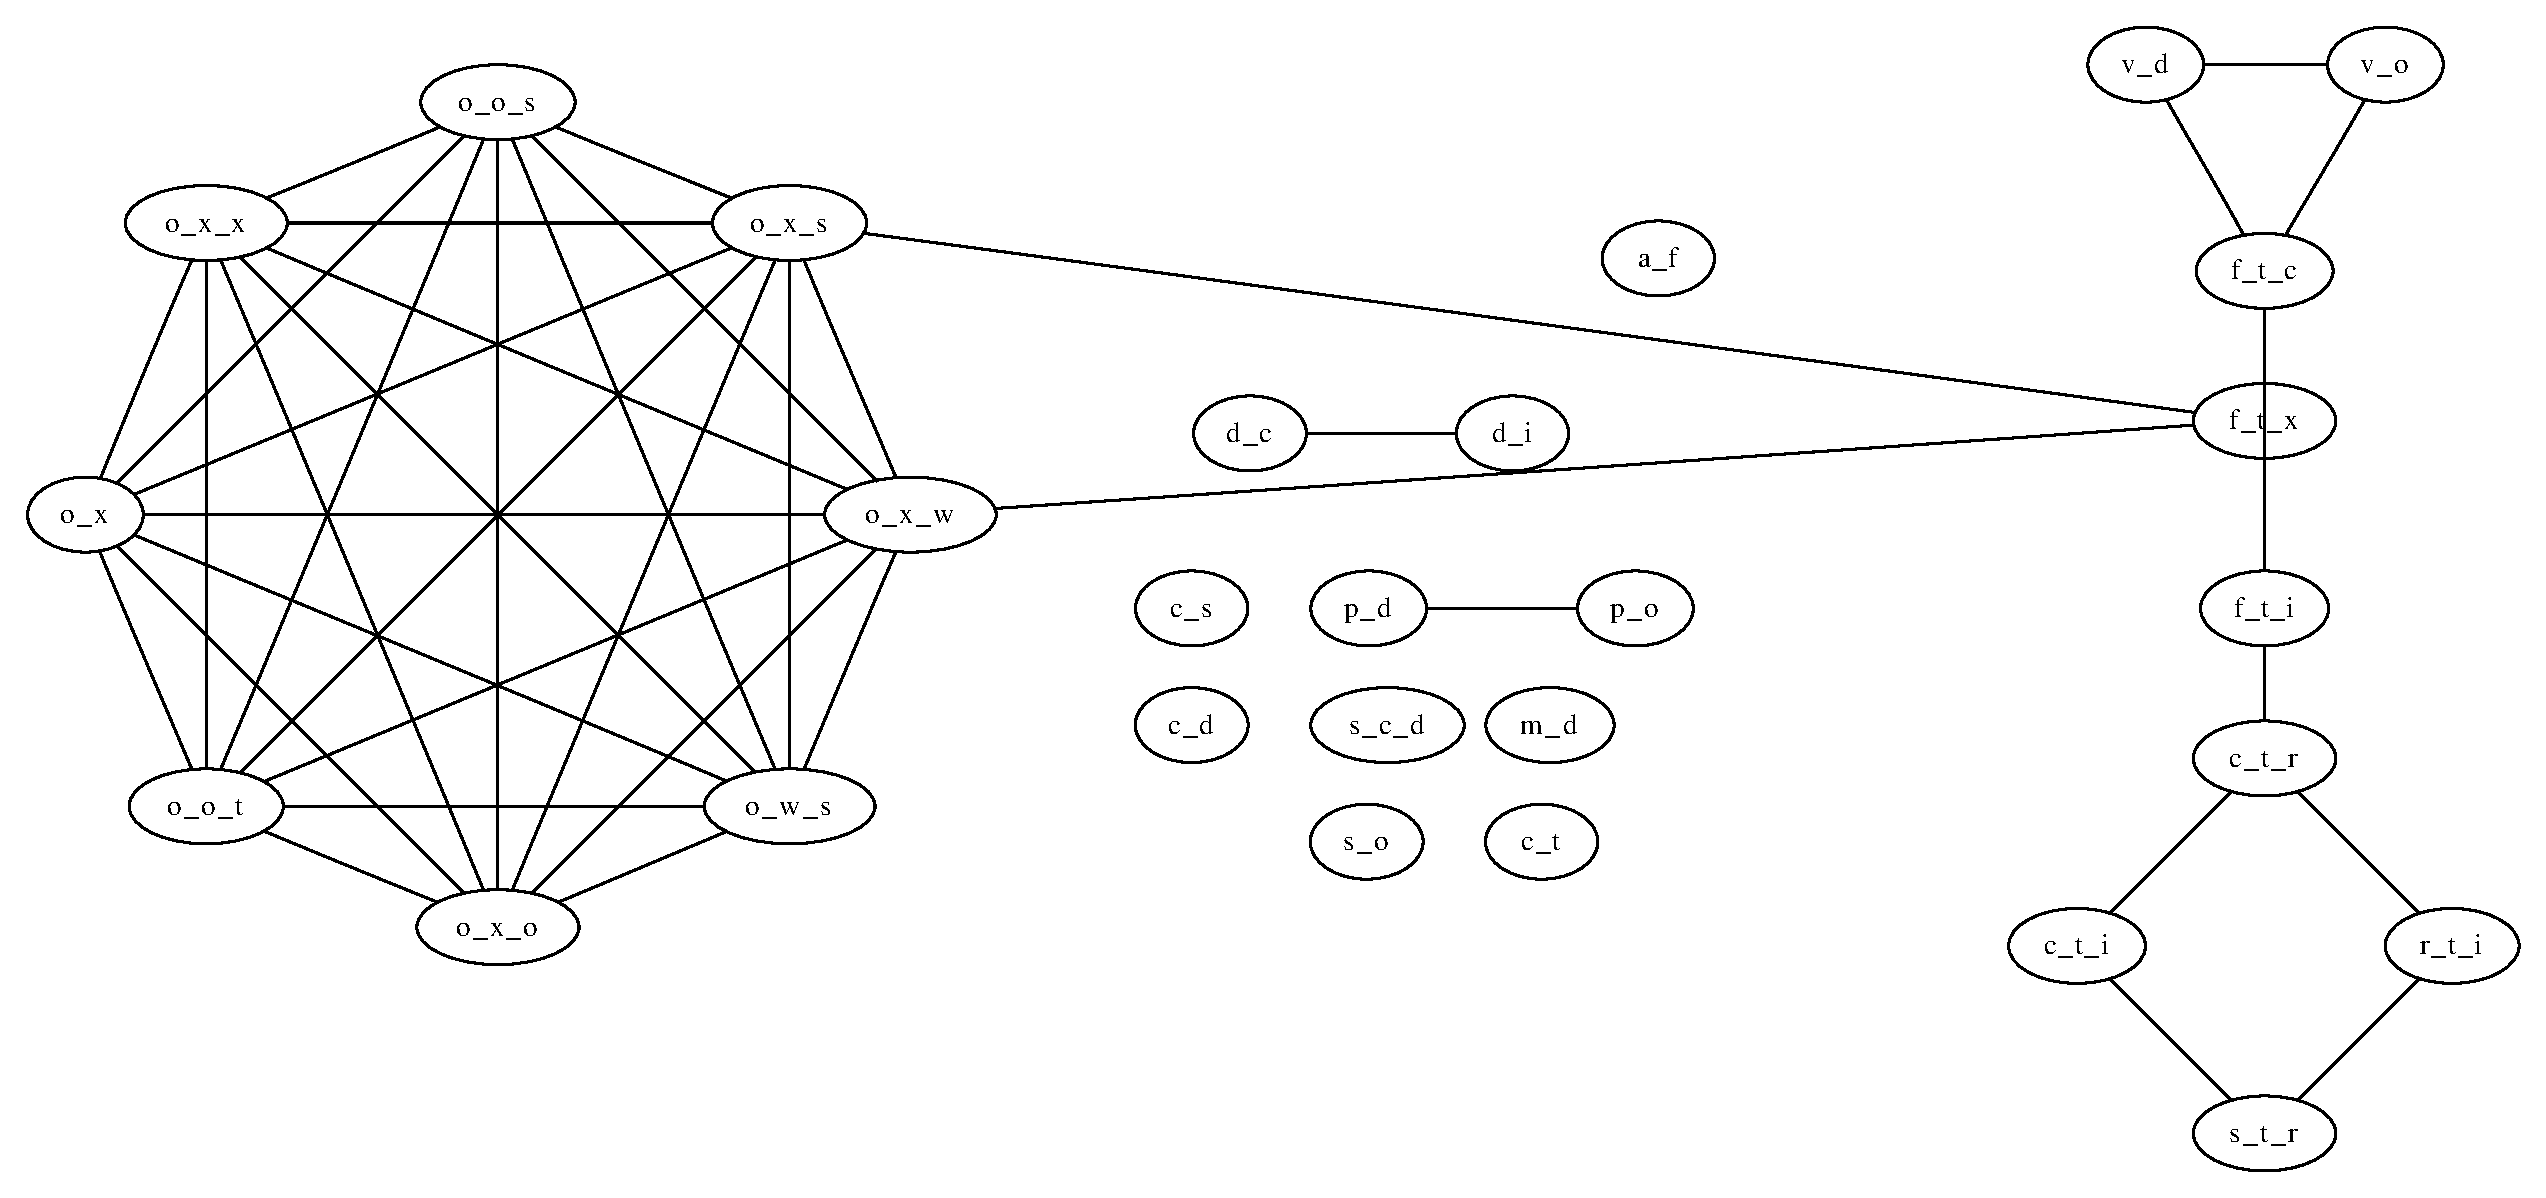
\includegraphics[width=0.45\textwidth]{images/experiments/data/realistic/OVA1}}
    \subfigure[\dataset{OVA2}]{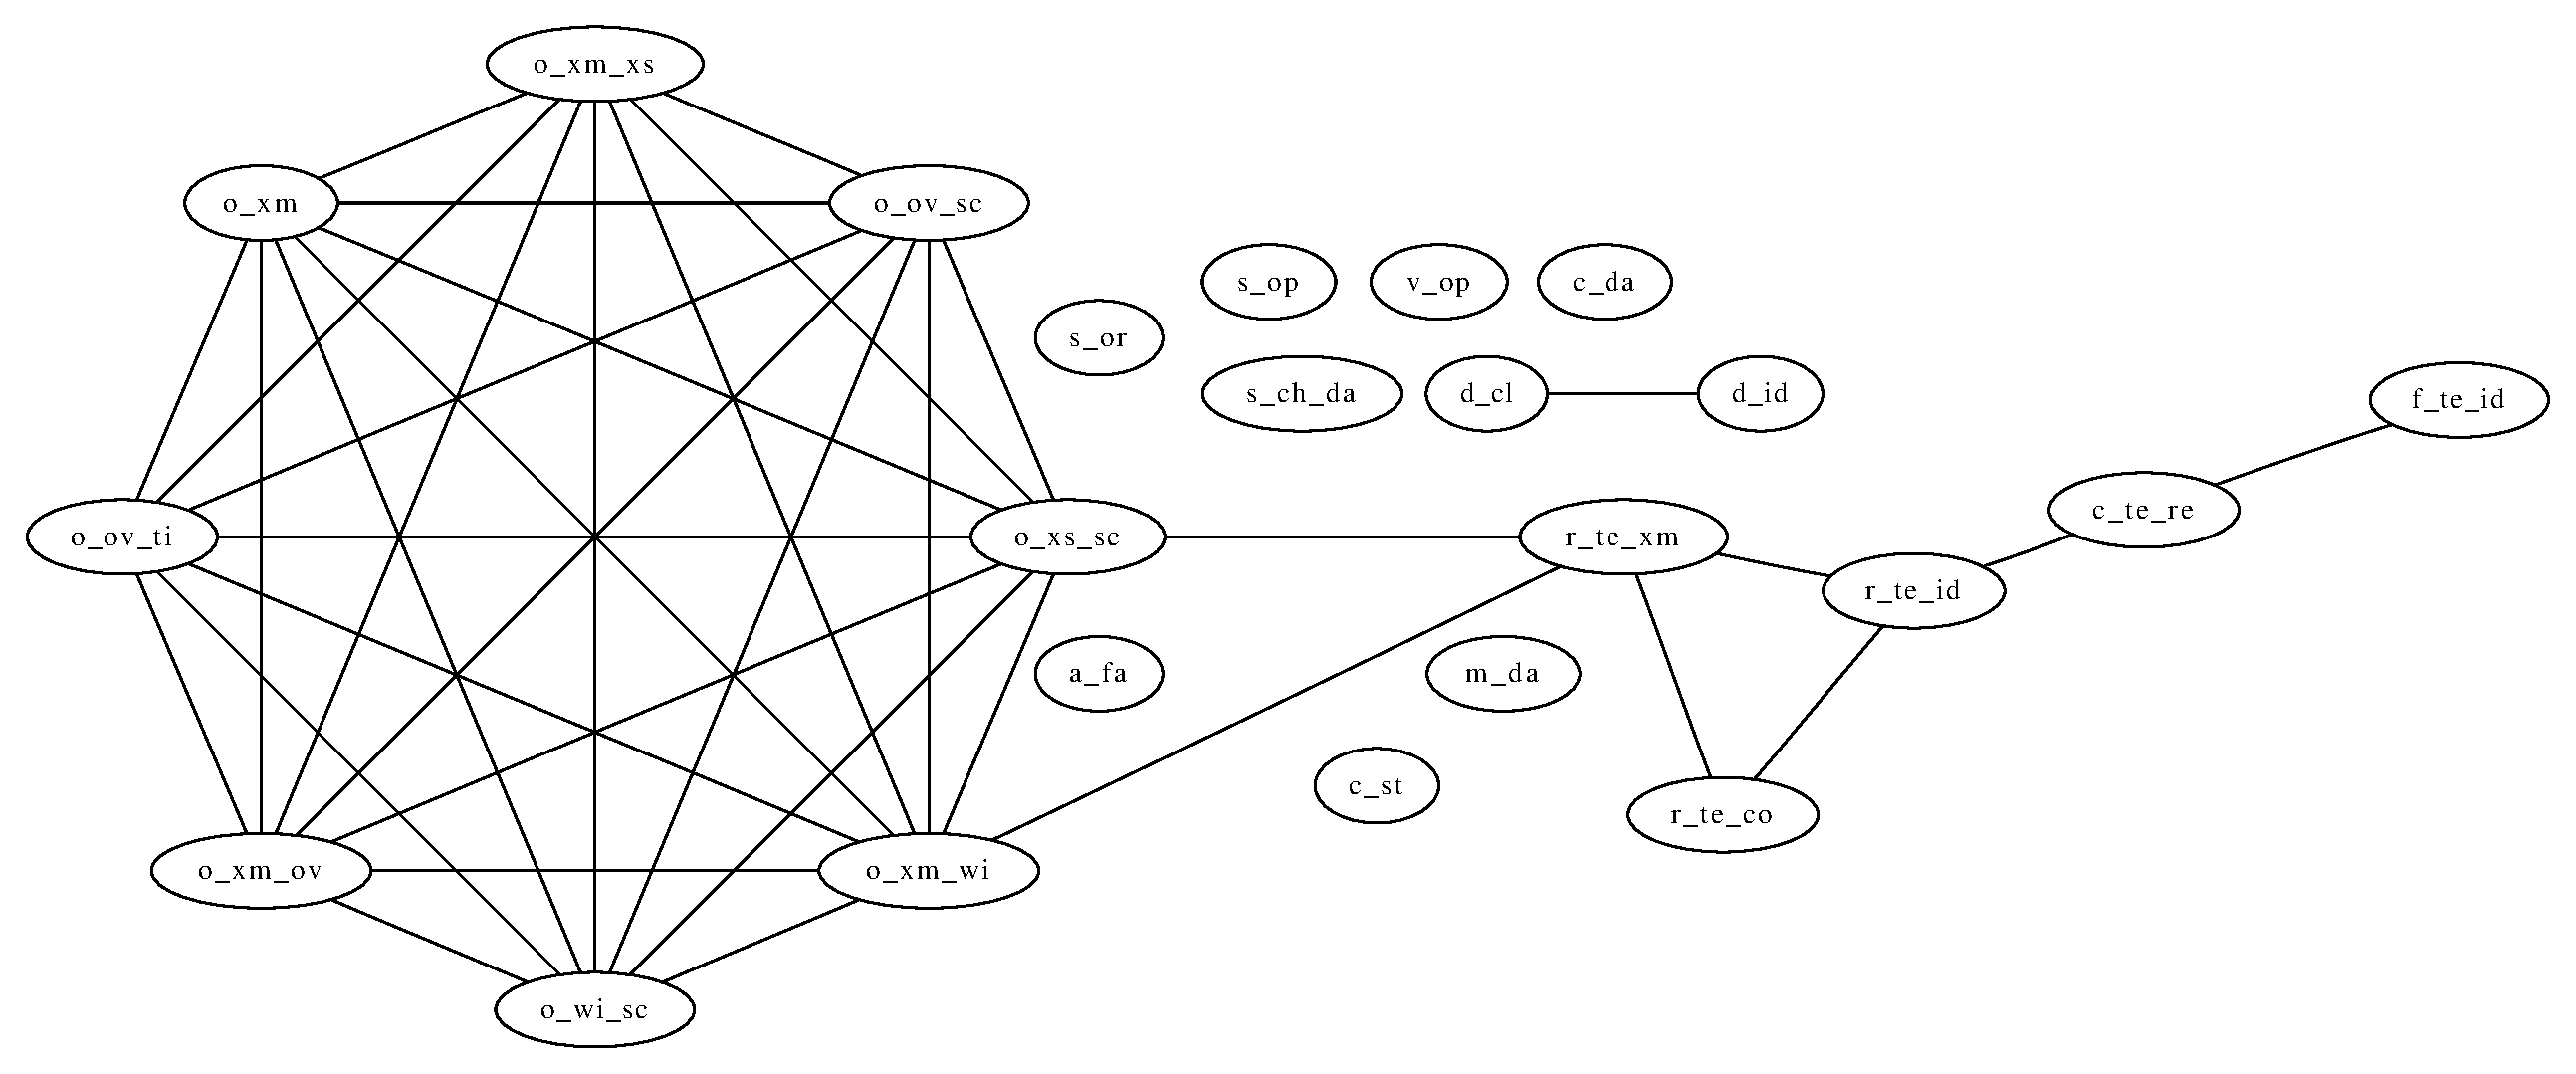
\includegraphics[width=0.45\textwidth]{images/experiments/data/realistic/OVA2}}
    \subfigure[\dataset{OVA3}]{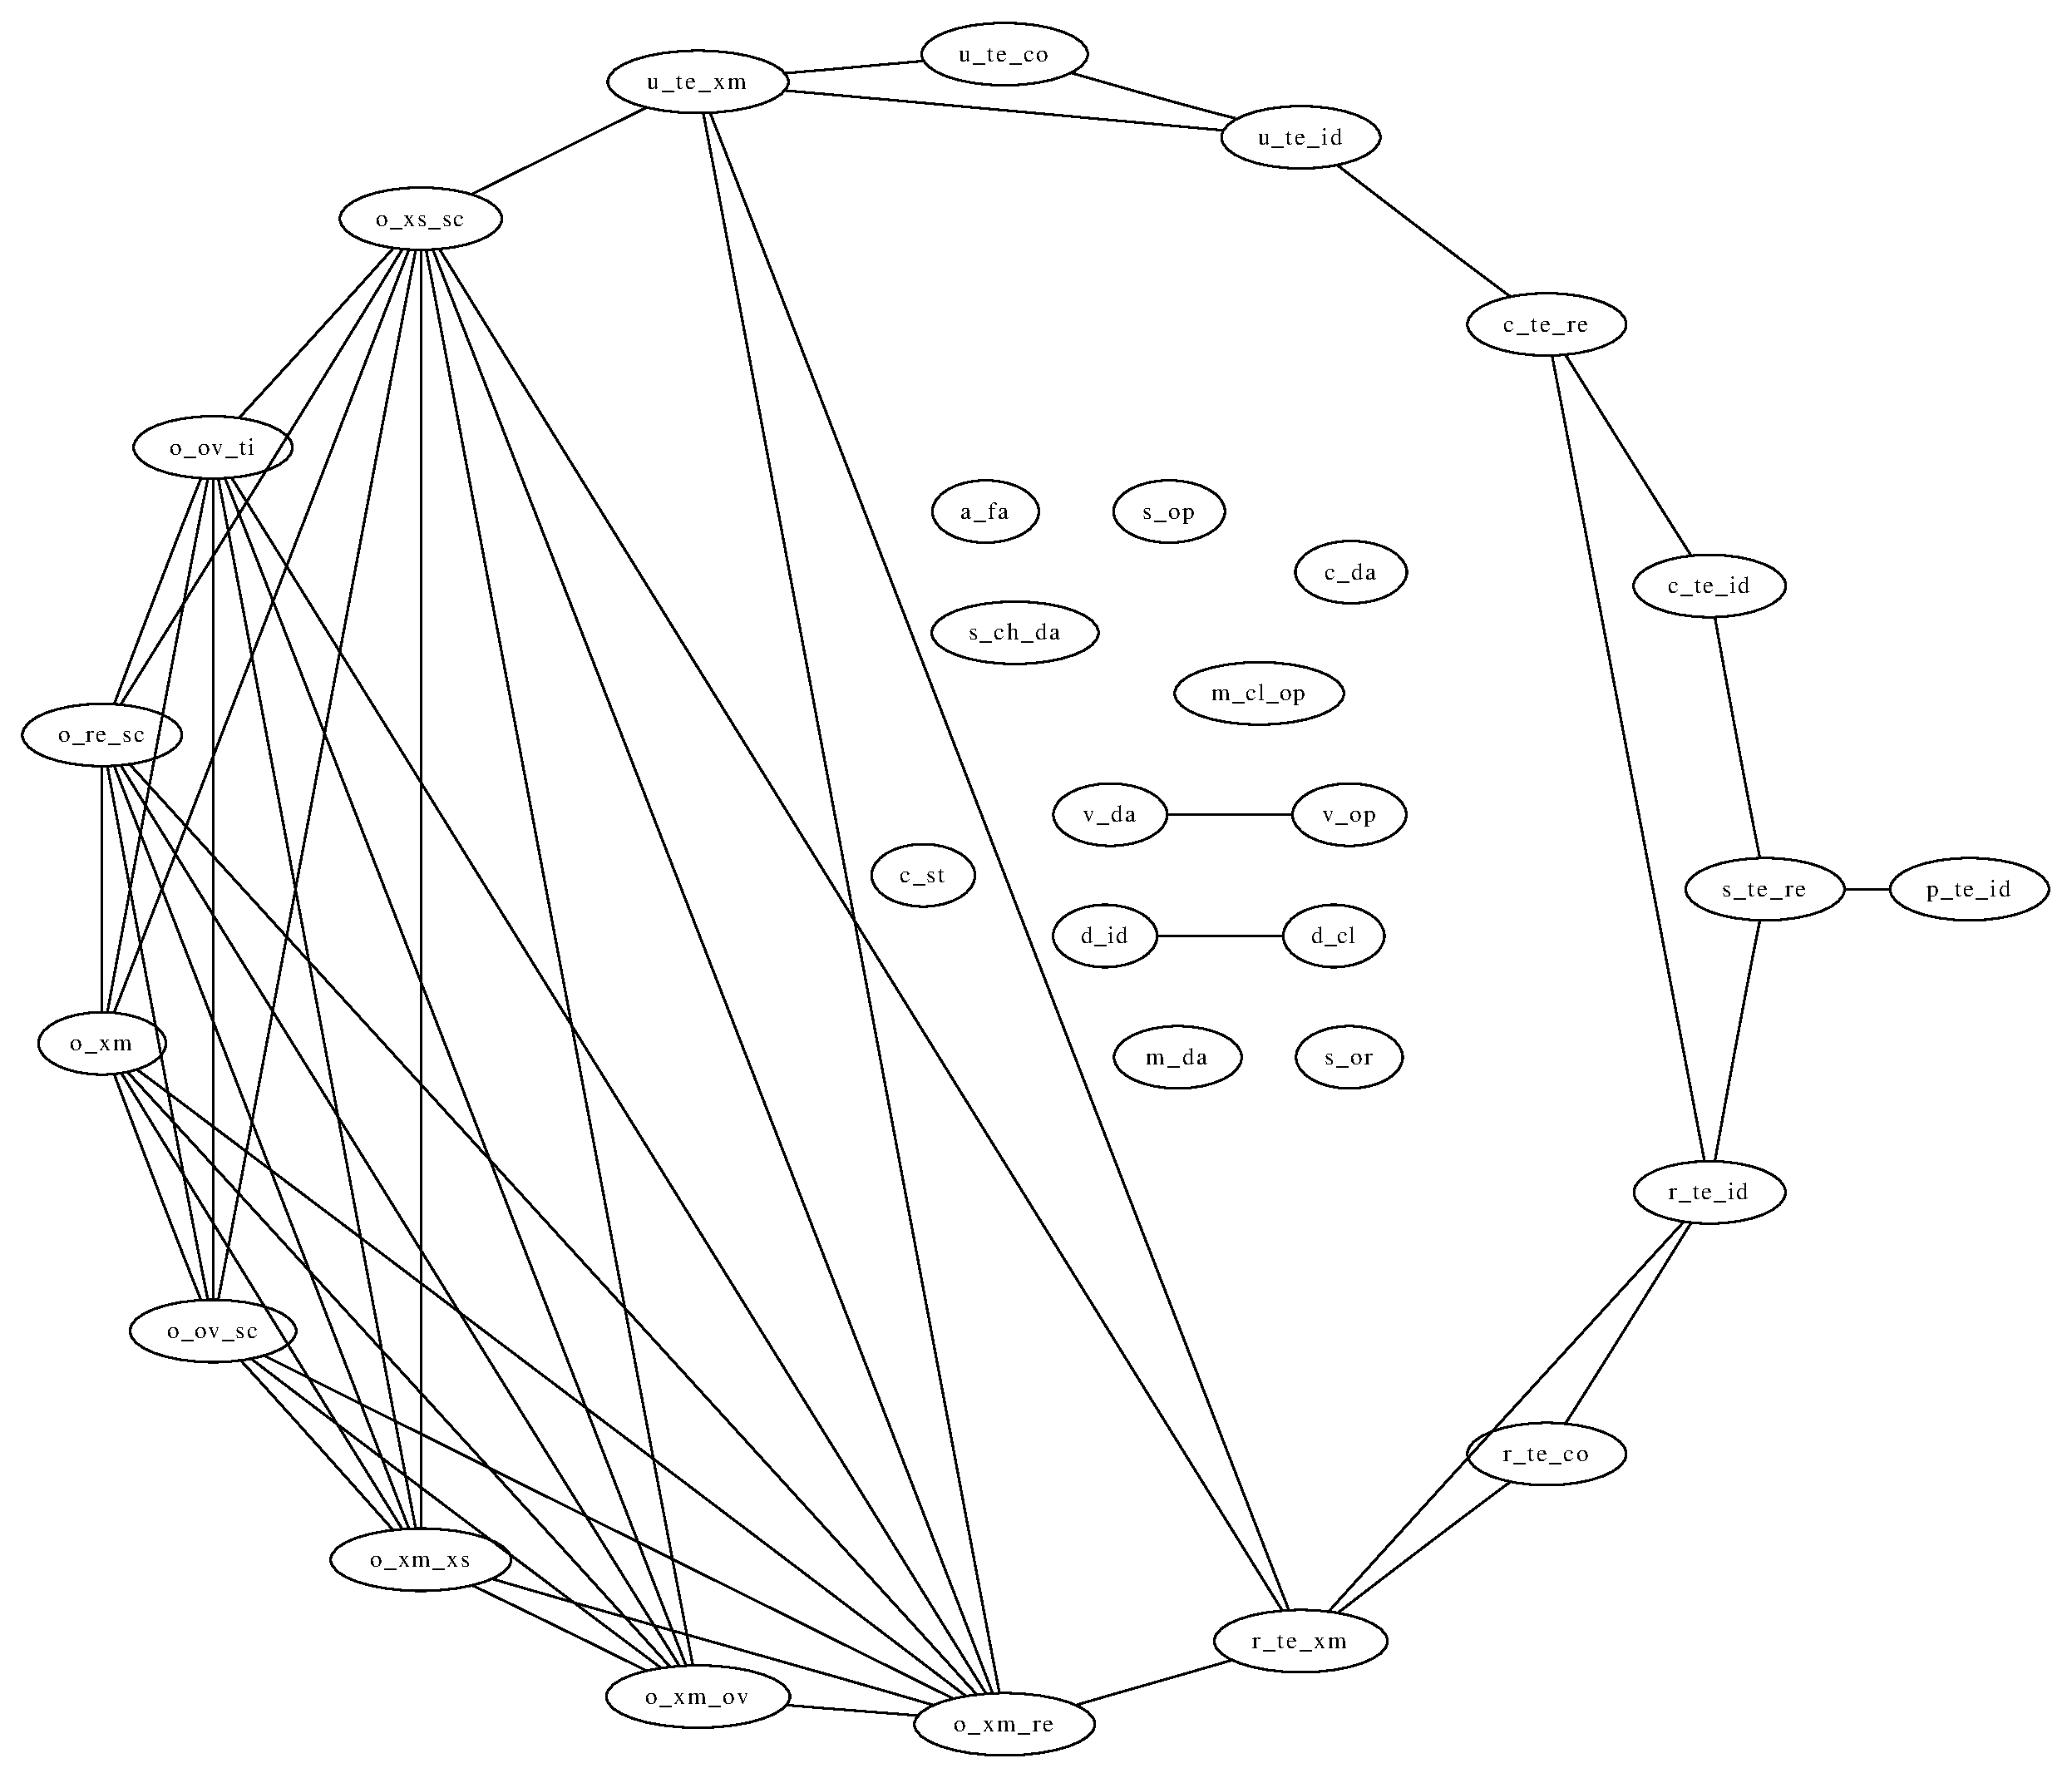
\includegraphics[width=0.45\textwidth]{images/experiments/data/realistic/OVA3}}
    \subfigure[\dataset{XMA-c}]{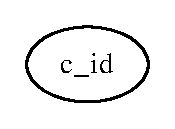
\includegraphics[width=0.08\textwidth]{images/experiments/data/realistic/XMA-c}}
    \subfigure[\dataset{XMA-p}]{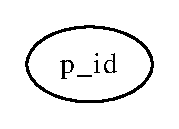
\includegraphics[width=0.08\textwidth]{images/experiments/data/realistic/XMA-p}}
    \subfigure[\dataset{XMD}]{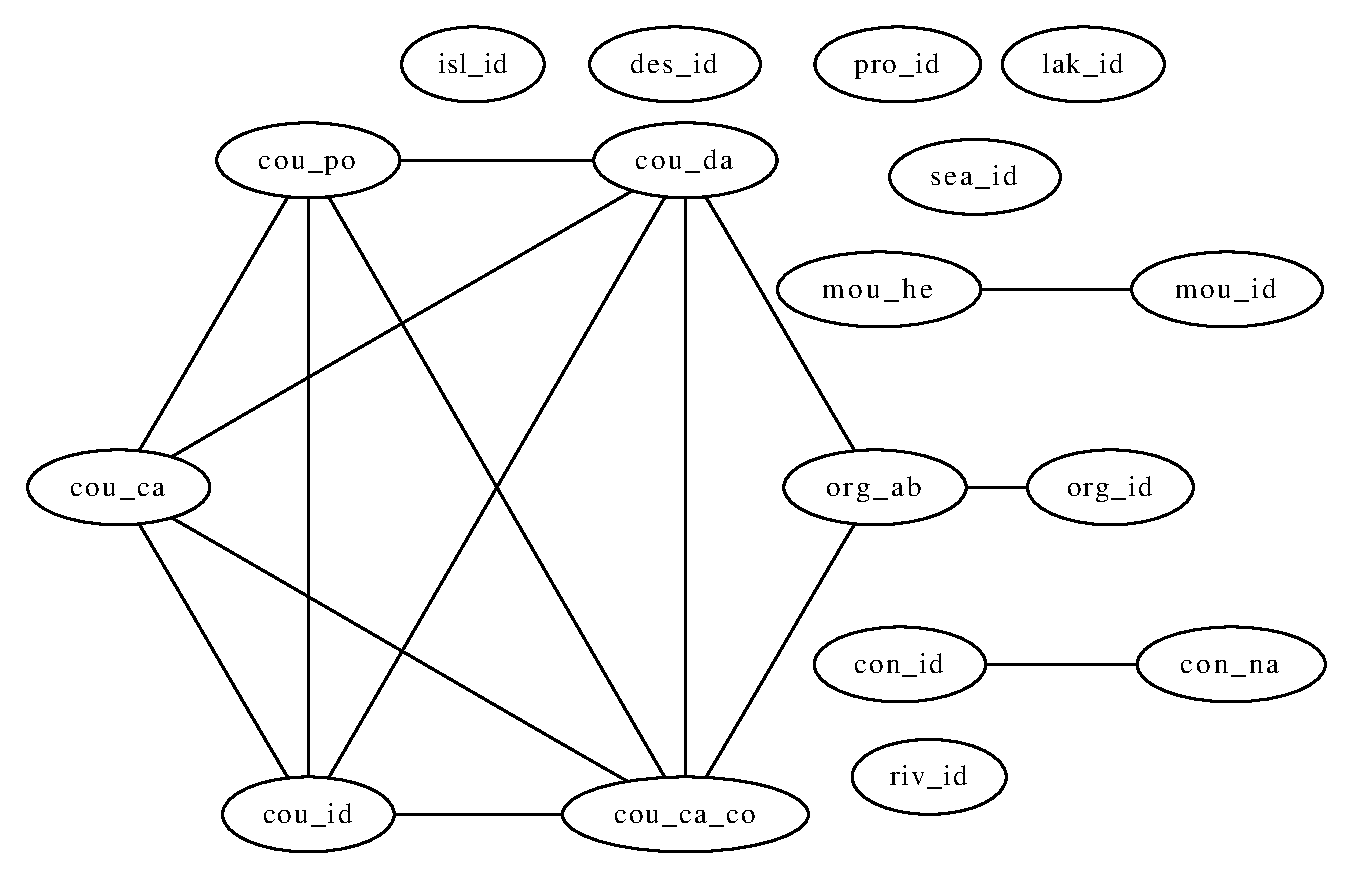
\includegraphics[width=0.45\textwidth]{images/experiments/data/realistic/XMD}}
\end{figure}

To interpret the data: \dataset{OVA*} sets have quite interesting and challenging graphs, but they are relatively small. We can consider them to be the ``typical'' representants.

On the other hand, the \dataset{XMA-*} sets are relatively huge, but trivial: their only candidate AM will just get picked and the heuristic will end. Therefore we will see the performance of the other components of the whole system, such as loading the data sets into memory representations.

Finally, the \dataset{XMD} set is relatively big and, at the same time, has non-trivial graph representation. In this case we should see a performance more balanced between processing and finding the ID set.

\subsection{Realistic data with artificial attributes}
\label{section-realistic-converted}

We used 2 data sets to convert, \dataset{MSH} and \dataset{NTH}. Unfortunately, the same problem with disclosure as in the previous case applies here, the DVD contains the anonymized version again. None of these sets had any attributes before the conversion. Their summary is Table \ref{table-experiments-data-converted}, their graphs are in Figure \ref{image-experiments-data-converted}.

To address the conversion: in case of \dataset{MSH} we found 2 elements with values resembling a key of the records contained in the file, and converted them to be attributes of these records using a simple XSL transformation. In the case of \dataset{NTH} we converted all the values in sub-elements of the record elements to be the attributes of the records.

This approach is useful, because as mentioned in Chapter \ref{chapter-research}, ID attributes are a special case of XML keys. We can use this approach to find XML keys: convert some ``suspicious'' data into attributes, find the optimal ID set and then create XML key based on this ID set.

\begin{table}
  \caption{List of realistic test data files with converted attributes}
  \bigskip
  \label{table-experiments-data-converted}
  \centering
  \begin{tabular}{l | r | c | c | l}
  	Name  & Size [kb] & $|V|$ & $|E|$ & Optimum \\
  	\hline
  	\dataset{MSH}  & 3 100.5 & 1 & 0 & 0.5416472778036296 \\
  	\dataset{NTH}  & 2 523.5 & 5 & 7 & 0.057918595422124436 \\
  \end{tabular}
\end{table}

\begin{figure}
  \caption{Realistic data with converted attributes}
  \label{image-experiments-data-converted}
  \centering
    \subfigure[\dataset{MSH}]{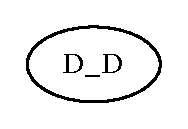
\includegraphics[width=0.08\textwidth]{images/experiments/data/converted/MSH}}
    \subfigure[\dataset{NTH}]{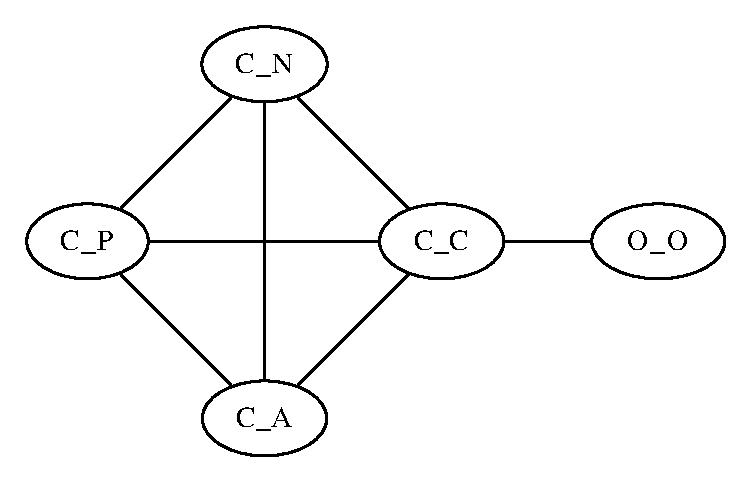
\includegraphics[width=0.45\textwidth]{images/experiments/data/converted/NTH}}
\end{figure}

In case of \dataset{MSH} we created 2 attributes, of which only one constituted a candidate AM. This is then the case similar to \dataset{XMA-*} sets: quite large data, yet only one trivial ID attribute to be found.

In case of \dataset{NTH} we introduced 8 attributes. Out of them 5 proved to be candidate AMs, with 7 edges constraining them. This means we have a relatively large set with considerably simple work to be done by the heuristics.

\subsection{Artificial data}

As soon as we started experimenting with the data coming from the real world, it was obvious that they are not complex enough. After we built the model, we got the most complex graphs of 31 vertices and 47 edges (see Table \ref{table-experiments-data-realistic}). Our solution is to approach the problem from the other side: in the end, we will be solving the equivalent of IS problem on a graph created from XML data. We will create the XML data to contain a more complex graph with a specific number of vertices and edges.

To demonstrate this, consider the following excerpt from an XML file:

\begin{scriptsize}
\begin{verbatim}
<graph>
  <vertex0 attr="-2968876296119015800"/>
  <vertex1 attr="1729745997570096518"/>
  <vertex2 attr="-9020549659620928934"/>
  ...
  <vertex99 attr="-7545982394508643394"/>

  <vertex82 attr="0"/><vertex21 attr="0"/>
  <vertex64 attr="1"/><vertex21 attr="1"/>
  <vertex44 attr="2"/><vertex2 attr="2"/>
  ...
  <vertex96 attr="99"/><vertex40 attr="99"/>
</graph>
\end{verbatim}
\end{scriptsize}

Our aim is to create a graph with approximately $v$ vertices and $e$ edges. First, we introduce $v$ elements with names \texttt{vertex0} - \texttt{vertex\{V-1\}}. To constitute an AM, they need an attribute \texttt{attr}, but with large enough random values, so that they do not conflict with others. Second, for each of the $e$ edges we choose two \texttt{vertex*} elements at random, and give them the same value of their \texttt{attr}. This will ensure they cannot share the same ID set, thus effectively creating the edge in the graph representation.

The respective pseudocode for this is provided in Algorithm \ref{listing-random-data}.

\begin{algorithm}
\caption{Random XML data creation}
\label{listing-random-data}
\begin{algorithmic}
\REQUIRE $v$ requested number of vertices
\REQUIRE $e$ requested number of edges
\ENSURE XML file content
\PRINT \texttt{<graph>}
\FOR{$i = 1 \to |V|$}
	\STATE $R \gets RANDOM$
	\PRINT \texttt{<vertex\textit{i} attr="\textit{R}">}
\ENDFOR
\FOR{$i = 1 \to |E|$}
	\STATE $v1 \gets RANDOM(|V|)$
	\STATE $v2 \gets RANDOM(|V|)$
	\PRINT \texttt{<vertex\textit{v1} attr="\textit{i}"> <vertex\textit{v2} attr="\textit{i}">}
\ENDFOR
\PRINT \texttt{</graph>}
\RETURN
\end{algorithmic}
\end{algorithm}

With this process it is possible to create as much data as needed, with any combination of $v$ and $e$ requested.

There is one characteristic that can describe random graphs like this, and that is the \textit{density}. This can be defined in various ways, we will use two different interpretations. The first is $\frac{|E|}{|V|}$, that is, how many edges are there for one vertex (multiplied by 2 we would get the average degree of the vertices).

The second, perhaps more interesting is $\frac{|E|}{E_{max}}$, where $E_{max} = \frac{|V|.(|V|-1)}{2}$. This is the density as the fraction of edges that are to all edges that could be in a complete graph with $|V|$ vertices.

We have created 3 sets to be used in experiments along with the realistic and converted sets, called \dataset{100-100}, \dataset{100-200} and \dataset{100-1000}. Note that the name is always in the form $v-e$.\\

All of the experimental data sets mentioned so far, realistic, converted and artificial alike will be referred to as \textit{official test data (sets)}.\\

Also, we will need data of comparably similar characteristics but varying size to study the effects of size on the run times of experiments. For this reason we created 11 more sets, from \dataset{0-0} as the trivial one to \dataset{100-500} as the largest one. These will be referred to as \textit{sized test data (sets)}. We wanted to keep the same density among these sets, so we picked the $\frac{|E|}{E_{max}}$ density interpretation for this.

A summary is provided in Table \ref{table-experiments-data-artificial} and Table \ref{table-experiments-data-artificial-size}; these tables contain 2 new columns: values of density in both interpretations we introduced. Some of the graph representations can be seen in Figure \ref{image-experiments-data-artificial}.

While studying the tables it becomes obvious that the actual numbers $|V|$ and $|E|$ do not match to the $v$ and $e$ in the names of the sets. This is because of the way the random generation algorithm works: it might pick the same edge twice, which will automatically render it unsuitable for the ID set. Because of the so-called Birthday paradox (see e.g. \cite{birthday}), this will happen more with higher $e$.

\begin{table}
  \caption{List of artificial test data files}
  \bigskip
  \label{table-experiments-data-artificial}
  \centering
  \begin{tabular}{l | r | c | c | c | c | l}
  	Name  & Size [kb] & $|V|$ & $|E|$ & $\frac{|E|}{|V|}$ & $\frac{|E|}{E_{max}}$ & Optimum \\
  	\hline
  	\dataset{100-100}  & 8.4  & 99 & 95  & 0.95 & 0.02 & 0.836666666666667 \\
  	\dataset{100-200}  & 13.0 & 96 & 174 & 1.81 & 0.04 & 0.726000000000000 \\
    \dataset{100-1000} & 49.5 & 93 & 754 & 8.11 & 0.16 & 0.380952380952381 \\
  \end{tabular}
\end{table}

\begin{table}
  \caption{List of ``sized'' artificial test data files}
  \bigskip
  \label{table-experiments-data-artificial-size}
  \centering
  \begin{tabular}{l | r | c | c | c | c | l}
	  Name  & Size [kb] & $|V|$ & $|E|$ & $\frac{|E|}{|V|}$ & $\frac{|E|}{E_{max}}$ & Optimum \\
  	\hline
  	\dataset{0-0}     & 0.2  & 0  & 0   & -    & -    & 0.0                \\
  	\dataset{10-5}    & 0.6  & 10 & 5   & 0.50 & 0.11 & 0.8500000000000002 \\
    \dataset{20-20}   & 1.7  & 18 & 13  & 0.72 & 0.08 & 0.7166666666666669 \\
    \dataset{30-45}   & 3.1  & 29 & 43  & 1.48 & 0.11 & 0.7083333333333334 \\
  	\dataset{40-80}   & 5.1  & 39 & 72  & 1.85 & 0.10 & 0.6950000000000002 \\
  	\dataset{50-125}  & 7.5  & 48 & 111 & 2.31 & 0.10 & 0.6566666666666666 \\
  	\dataset{60-180}  & 10.4 & 58 & 157 & 2.71 & 0.09 & 0.6214285714285716 \\
  	\dataset{70-245}  & 13.8 & 67 & 205 & 3.06 & 0.09 & 0.5982142857142856 \\
  	\dataset{80-320}  & 17.6 & 76 & 261 & 3.43 & 0.09 & 0.5791666666666667 \\
  	\dataset{90-405}  & 21.9 & 86 & 352 & 4.09 & 0.10 & 0.528888888888889  \\
  	\dataset{100-500} & 26.7 & 91 & 388 & 4.26 & 0.09 & 0.4981818181818182 \\
  \end{tabular}
\end{table}

\begin{figure}
  \caption{Artificial data}
  \label{image-experiments-data-artificial}
  \centering
    \subfigure[\dataset{48-80}]{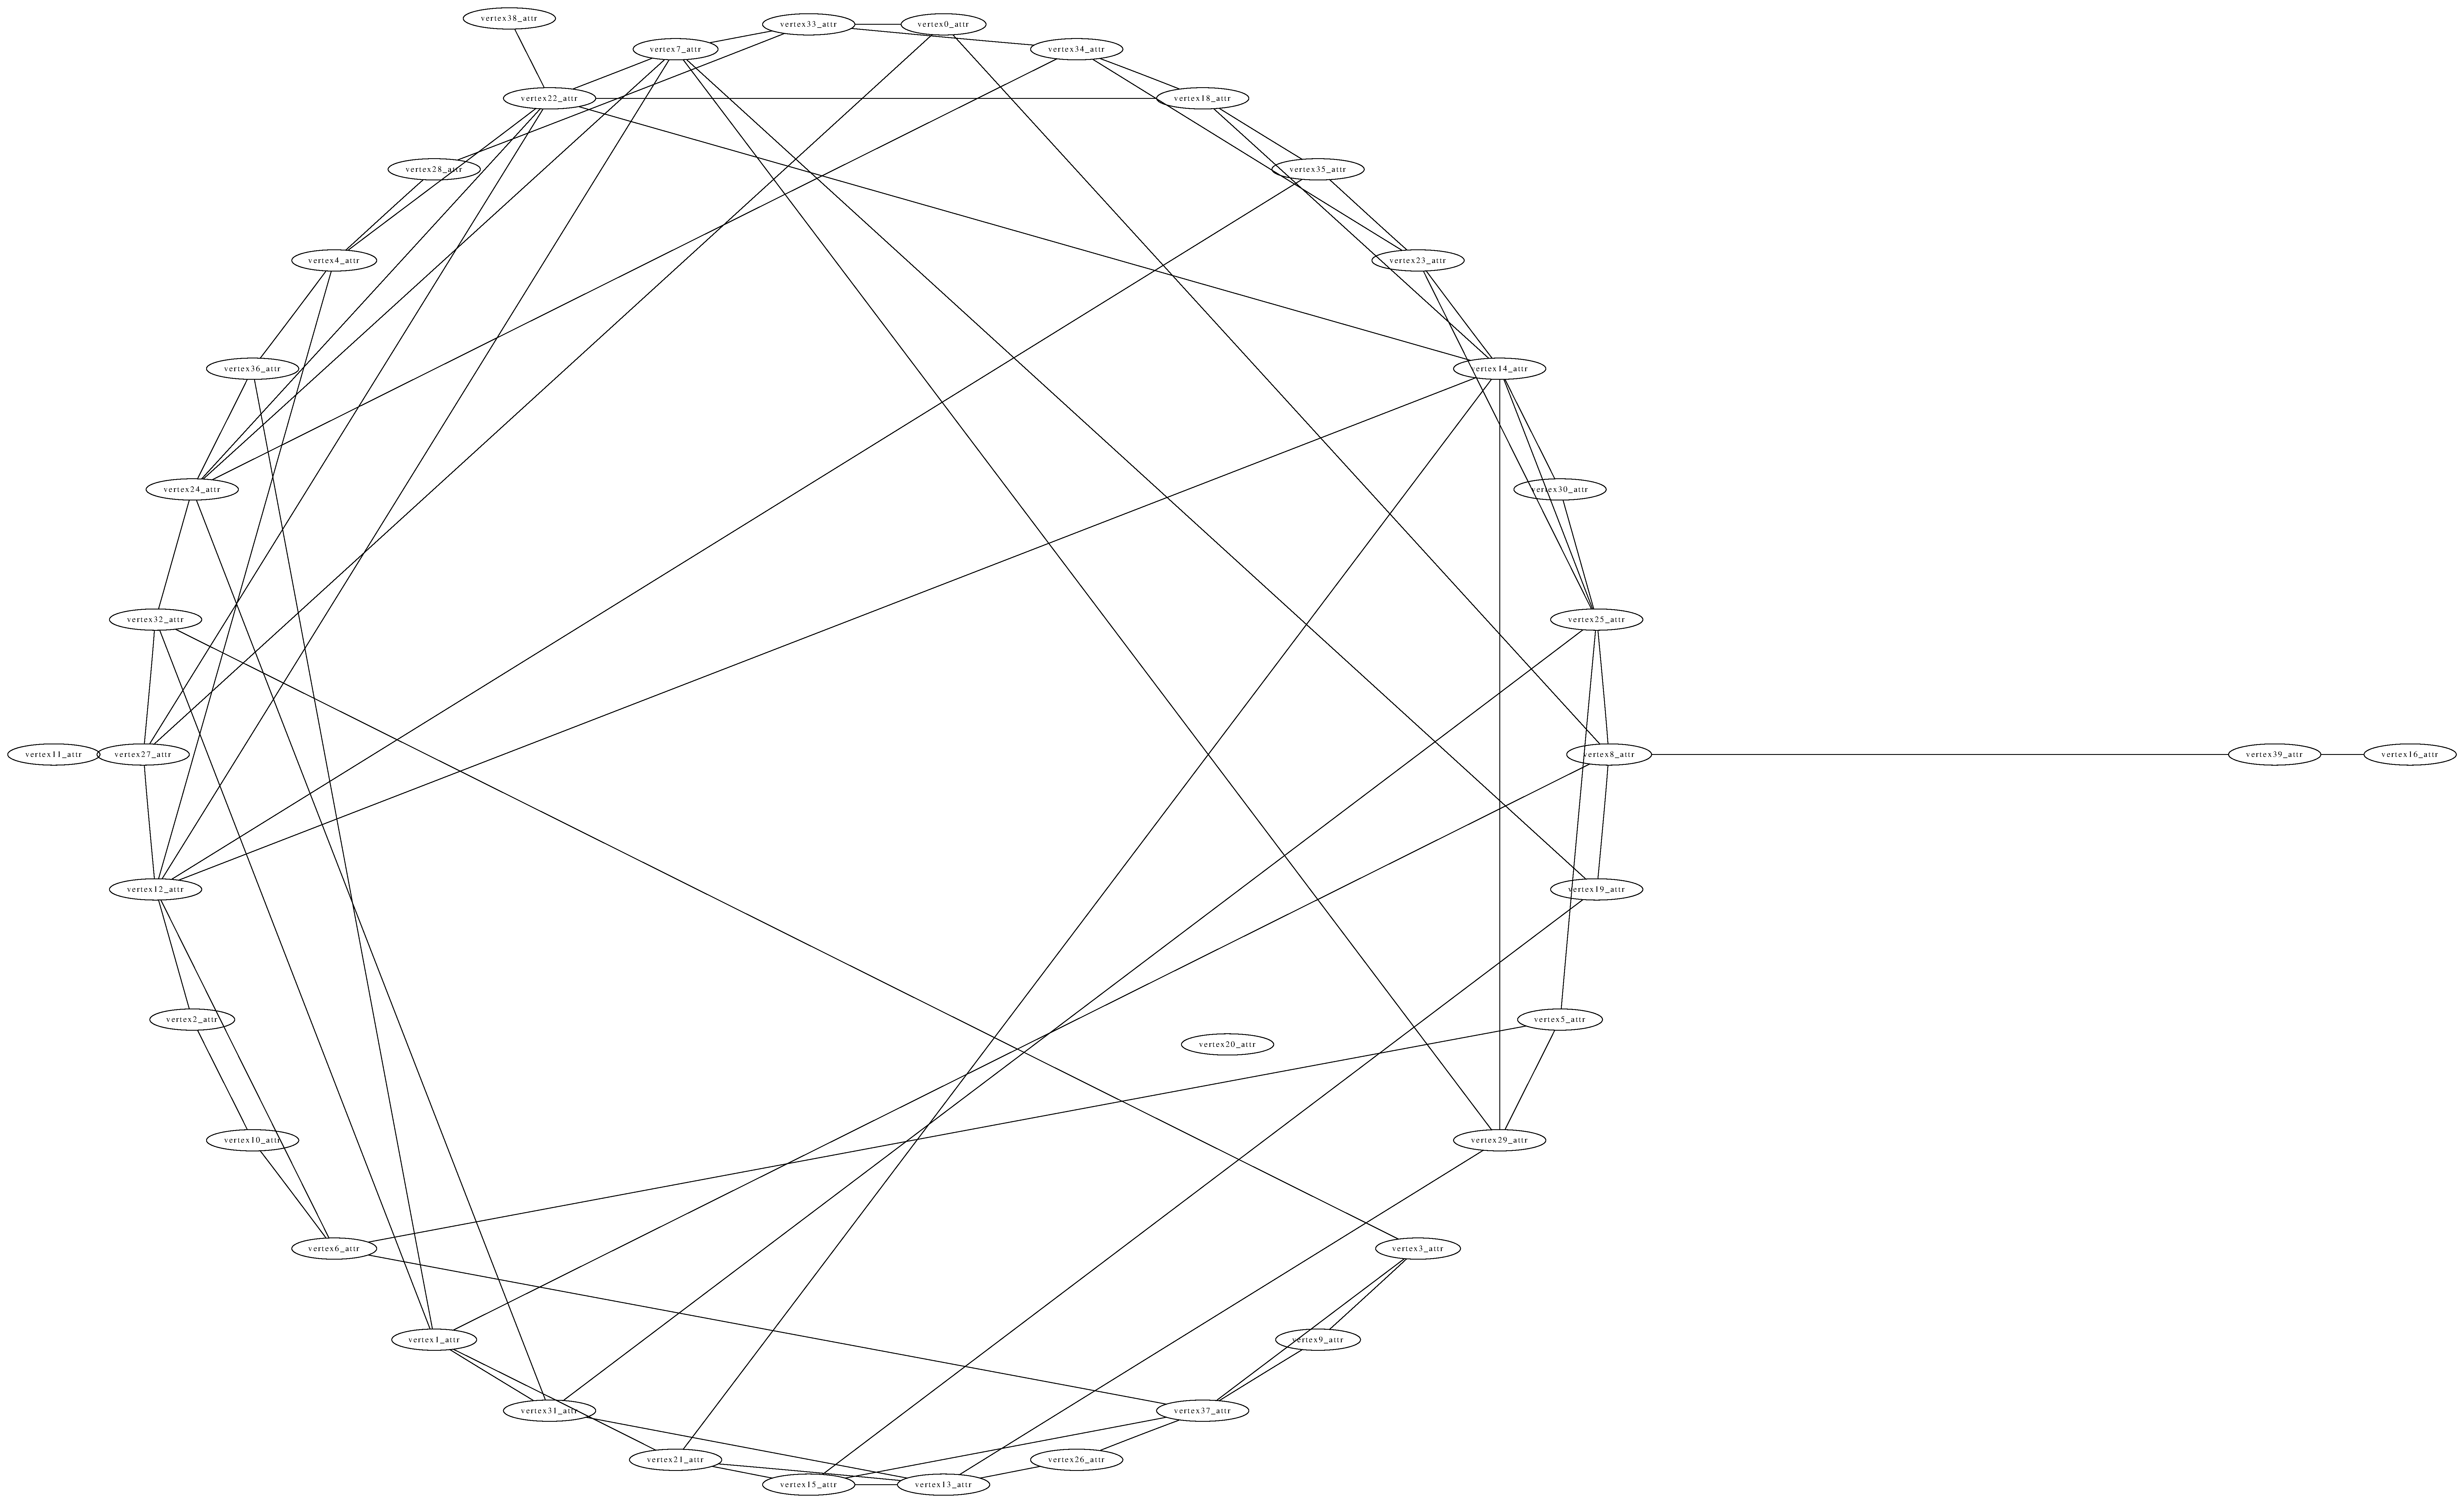
\includegraphics[width=\textwidth]{images/experiments/data/artificial/size/40-80}}
    \subfigure[\dataset{70-245}]{
\includegraphics[width=.8\textwidth]{images/experiments/data/artificial/size/70-245-fixed}}
\end{figure}

To interpret Tables \ref{table-experiments-data-artificial} and \ref{table-experiments-data-artificial-size}: we get 3 sets of different sizes and densities in the first one. The $|V|$ and $|E|$ numbers are orders of magnitude higher than in any realistic (or converted) data set we are using.

In the second table we aimed for the $\frac{|E|}{E_{max}}$ density of $0.1 = 10\%$, and we can see that this was indeed achieved. There is an interesting observation to be made here: the optimum is steadily decreasing with the increasing overall graph size. This intuitively suggests that the maximum quality theoretically achievable is related to the $\frac{|E|}{|V|}$ density, not to the one we fixed. Exploration of this phenomenon is beyond the scope of this thesis.

Note that the artificial data we used in experiments can be found on the DVD enclosed with this work.

\section{Experimental Setup}

As was mentioned before, we will use an extension to the jInfer framework called \jmodule{IDSetSearch}. Please see Appendices \ref{appendix-jInfer} and \ref{appendix-iss} for more detailed information on these two pieces of software.\\

We now have to introduce a few notions before moving forward to the description of our experiments. In the following text, words \textit{experiment} and \textit{experimental} in various phrases (\textit{experiment X}, \textit{experimental Y}) will be used interchangeably.\\

\textit{Experiment parameters} are the following ones.
\begin{itemize}
	\item All the parameters in all the heuristics.
	\item The specific way in which the heuristics are chained.
	\item Parameters $\alpha$ and $\beta$ in the weight (quality) measurement.
	\item Initial pool size.
	\item The termination criteria.
	\item The input XML file.
	\item Known optimum for this file and $\alpha$, $\beta$.
\end{itemize}

An \textit{experiment instance}, or \textit{experiment configuration}, is one specific setting of all experiment parameters.\\

And finally, one or more experiment configurations, regardless whether their parameters differ, constitute an \textit{experiment set}.

\subsection{Grammar and Model Creation}

This section will briefly describe the process by which an input data set is processed to obtain the AM model as described in Section \ref{section-definitions-ams}.\\

An input data set is a single XML file on the filesystem; however, there is a straightforward extension to multiple files conforming to the same schema. The first step in this process is to use jInfer's module \jmodule{BasicIGG} module (see \cite{basiciggdoc} for details) to obtain a list of rules - an \textit{initial grammar} (IG). \nomenclature{IG}{Initial Grammar}
Please see \cite{archdoc} for detailed specification of IG format.\\

The second step is to convert the grammar into the AM model. This is done by a linear scan and retrieving a so-called \textit{flat} representation. This consists of a list of tuples in the following format.

\begin{center}
\textit{(element name, attribute name, attribute value)}
\end{center}

There is a tuple for every attribute node with a value found in the initial grammar. Note that the information about the context in which the element was originally found is lost - but this is not a problem with regard to the definition of XML ID attributes. Furthermore, tuples in flat representation do not need to be unique.\\

The model now has to be able to return the list of all attribute mappings and their respective images. This is achieved by simply grouping the flat representation by the pair \textit{(element name, attribute name)} and aggregating all attribute values for each such pair. Another responsibility of the model is to return the list of \textit{types} - that is simply the list of unique \textit{element name}s.

\subsubsection{Example}

Recall the following XML file fragment from Chapter \ref{chapter-definitions}.
\begin{verbatim}
<x>
  <y a="1" b="2"/>
  <y a="3" c="4"/>
  <y/>
  <z a="1"/>
</x>
\end{verbatim}

Its IG representation is the following set of IG rules.

\begin{eqnarray*}
	x & \to & y, y, y, z \\
	y & \to & @a, @b \\
	y & \to & @a, @c \\
	y & \to & empty\_concatenation \\
	z & \to & @a \\
\end{eqnarray*}

The flat representation will consist of the following set of tuples.

\begin{eqnarray*}
(y, a, 1) \\
(y, b, 2) \\
(y, a, 3) \\
(y, c, 4) \\
(z, a, 1) \\
\end{eqnarray*}

Attribute mappings in this model will be $(y, a)$, $(y, b)$, $(y,c)$ and $(z,a)$. Their images will be $(1,3)$, $(2)$, $(4)$ and $(1)$, respectively. The list of types in this model will be $(y,z)$.

\subsection{Hardware and Software}

We will use the following configuration when conducting our experiments.

\begin{verbatim}
Intel Core 2 Duo processor @ 2.33 GHz
4 GB DDR2 RAM
Windows 7 SP1 64bit
Java SE Runtime Environment (build 1.6.0_26-b03)
Java HotSpot 32-Bit Client VM (build 20.1-b02)
GLPK version 4.45 (Cygwin)
GLPK version 4.34 (native)
\end{verbatim}

\subsection{Methodology}

We will attempt to protect our experiment from the influence of the environment as much as reasonably possible. First of all, NetBeans running the experiments is the only relevant program running in the system while the experiments are performed. Unfortunately, NetBeans itself is quite a large environment, and we would most certainly get more reliable results if we could run our experiments outside of it. This improvement is left for the future work.

Also, every experimental configuration is run 50 times so that the effects of any events adversely affecting our results (e.g. OS deciding to run some house cleaning) will be averaged out. Whenever possible, we will use boxplots instead of a simple average (or average and variance) to present results of these multiple runs.

\subsection{Measuring the Time}

Whenever it is necessary to measure the duration of an operation, we will use the \texttt{System.nanoTime()} built-in function. The result cannot be interpreted in an absolute manner, but by subtracting the time at the start from the time at the end, we can get a reasonably reliable measurement.

\subsection{Obtaining the Results}

Every run of an experiment produces a trace such as the one presented and commented on in Appendix \ref{appendix-trace}. We can get all the information relevant to that experiment run from this trace alone. An experimental set will produce a number of these traces and store them in plain text files in a folder. Parsing these files to aggregate and collate them might be a tedious task even using tools like \texttt{sed} and \texttt{grep}, so some of the experiment sets directly output tabular data in format recognized by GnuPlot \cite{gnuplot}, which we use to plot charts found in this work.

\subsection{Reading Boxplots}

To present a set of measurements obtained by iteratively running an experiment we shall prominently use the \textit{boxplot} chart. Because we use boxplots produced by GnuPlot, let us quote its manual \cite{gnuplot-manual} for the exact definition.

\begin{quote}
Quartile boundaries are determined such that 1/4 of the points have a value equal or less than the first quartile boundary, 1/2 of the points have a value equal or less than the second quartile (median) value, etc. A box is drawn around the region between the first and third quartiles, with a horizontal line at the median value. Whiskers extend from the box to user-specified limits. Points that lie outside these limits are drawn individually.
\end{quote}

The ``user-specified limits'' of whiskers are set to default value, let us quote from the manual again.

\begin{quote}
By default the whiskers extend from the ends of the box to the most distant point whose y value lies within 1.5 times the interquartile range.
\end{quote}

\section{Experimental Results}

\subsection{Grammar and Model Generation}
\label{section-grammar-model-timing}

%         NB class GrammarModelTiming

The first experiment set will try to establish how long it takes to extract the IG % TODO IG -> nomenclature
from the input XML file and how long does it take to create the AM model from this IG. For now, we will not be running or measuring any heuristics.

\begin{center}
\bigskip
\begin{tabular}{| l | l |}
  \hline
  \hline
  Input data        & all official and sized test data sets \\
  Iterations        & 50 \\
  Pool size         & not applicable \\
  $\alpha$, $\beta$ & not applicable \\
  CH                & not applicable \\
  IHs               & not applicable \\
  \hline
\end{tabular}
\bigskip
\end{center}

The experimental set will contain $50 * (11 + 11) = 1100$ configurations: 50 iterations for 11 test data sets plus 11 sized test data sets. There will be no CHs or IHs. We will be gathering the timing data for IG extraction and model generation in GnuPlot format.\\

\begin{table}
  \caption{Grammar Extraction and Model Creation Times}
  \bigskip
  \label{table-experiments-grammar-model-timing}
  \centering
  \begin{tabular}{l || l | l || l | l || l | l}
    Data set & GE & GE & MC & MC & Tot & Tot \\
     & avg [ms] & stdev & avg [ms] & stdev & avg [ms] & stdev \\
    \hline
    \dataset{OVA1}     & < 10 & - & < 10 & - & < 10 & - \\
    \dataset{OVA2}     & < 10 & - & < 10 & - & < 10 & - \\
    \dataset{OVA3}     & 42.94 & 19.8509 & 60.92 & 27.0848 & 103.86	& 31.6911 \\
    \dataset{XMA-c}    & 140.32 &	33.2618 &	90.24 &	45.8803 & 230.56 & 56.2633 \\
	\dataset{XMA-p}    & 7518.82 &	922.8882 &	10135.46 &	502.8997 & 17654.28	& 1353.8794 \\
	\dataset{XMD}      & 979.18 &	307.1760 &	563.04 & 341.4697 & 1542.22	& 134.6883 \\
	\dataset{MSH}      & 570.24 &	167.1119 &	225.48 &	90.6775 & 795.72 & 161.8340 \\ 
	\dataset{NTH}      & 328.36 & 118.3766 &	1074.9 &	155.5604 & 1403.26 & 137.8695 \\
	\dataset{100-100}  & < 10 & - & < 10 & - & < 10 & - \\
	\dataset{100-200}  & < 10 & - & < 10 & - & < 10 & - \\
	\dataset{100-1000} & 18.34 & 10.2372 & 18.84 & 1.0373 & 37.18 & 9.9338 \\
	\dataset{0-0}      & < 10 & - & < 10 & - & < 10 & - \\
	\dataset{10-5}     & < 10 & - & < 10 & - & < 10 & - \\
	\dataset{20-20}    & < 10 & - & < 10 & - & < 10 & - \\
	\dataset{30-45}    & < 10 & - & < 10 & - & < 10 & - \\
	\dataset{40-80}    & < 10 & - & < 10 & - & < 10 & - \\
	\dataset{50-125}   & < 10 & - & < 10 & - & < 10 & - \\
	\dataset{60-180}   & < 10 & - & < 10 & - & < 10 & - \\
	\dataset{70-245}   & < 10 & - & < 10 & - & < 10 & - \\
	\dataset{80-320}   & < 10 & - & < 10 & - & 12.48 & 8.3574 \\
	\dataset{90-405}   & < 10 & - & < 10 & - & 15.88 & 10.3778 \\
	\dataset{100-500}  & < 10 & - & < 10 & - & 18.74 &	8.8889 \\
  \end{tabular}
\end{table}

Results are in Table \ref{table-experiments-grammar-model-timing}. We are presenting the average grammar extraction (GE) times and their standard deviation, the same for model creation (MC) and total (sum of these two, Tot) times. For many data sets the average time is less than 10 ms: this is not enough to be precise and we don't calculate the standard deviation in these cases.

We can see from the results that for most data sets their model can easily be created under around one second, only in case of the biggest set \dataset{XMA-p} (13 MB) this takes some 17 seconds. We can conclude that grammar and model creation times are not a bottleneck for now. Heuristics run times will be order of magnitude higher.

\subsubsection{GLPK Interface Timing}

%         NB class GlpkInterfaceTiming

A related problem is how long it takes to create input for GLPK and then parse its results. We will use the same test data sets as in the previous case, but now we will gather times needed to communicate with GLPK.\\

\begin{table}
  \caption{GLPK Interface Times}
  \bigskip
  \label{table-experiments-glpk-timing}
  \centering
  \begin{tabular}{l || l | l || l | l || l | l}
	Data set & IC & IC & OP & OP & Tot & Tot \\
     & avg [ms] & stdev & avg [ms] & stdev & avg [ms] & stdev \\
	\hline
	\dataset{OVA1} & 36.46 & 66.8517 & 49.8 & 114.0687 & 86.26 & 150.1044 \\
	\dataset{OVA2} & 39.52 & 75.8210 & 48.8 & 102.4484 & 88.32 & 154.9596 \\
	\dataset{OVA3} & 34.1 & 74.1838 & 38.62 & 89.3772 & 72.72 & 134.7295 \\
	\dataset{XMA-c} & 40.88 & 88.6632 & 33.84 & 65.8636 & 74.72 & 127.7338 \\
	\dataset{XMA-p} & 36.54 & 70.7436 & 49.24 & 101.2412 & 85.78 & 145.2092 \\
	\dataset{XMD} & 37.98 & 69.2719 & 32.88 & 70.2173 & 70.86 & 114.6692 \\
	\dataset{MSH} & 40.42 & 91.9885 & 36.52 & 72.1018 & 76.94 & 138.6198 \\
	\dataset{NTH} & 36.02 & 66.3403 & 38.06 & 88.8244 & 74.08 & 128.9974 \\
	\dataset{100-100} & 46.5 & 103.3929 & 46.92 & 89.7049 & 93.42 & 158.7267 \\
	\dataset{100-200} & 42.34 & 96.1204 & 38.22 & 90.0284 & 80.56 & 152.6534 \\
	\dataset{100-1000} & 32.92 & 64.4534 & 42.1 & 89.4546 & 75.02 & 127.8541 \\
	\dataset{0-0} & 46.8 & 123.5183 & 46.92 & 102.2601 & 93.72 & 181.5228 \\
	\dataset{10-5} & 40.06 & 75.7370 & 40.1 & 72.4851 & 80.16 & 126.7135 \\
	\dataset{20-20} & 33.72 & 70.7263 & 34.1 & 66.2781 & 67.82 & 116.3783 \\
	\dataset{30-45} & 38.26 & 71.7549 & 45.94 & 110.1284 & 84.2 & 155.7594 \\
	\dataset{40-80} & 37.06 & 67.0024 & 49.26 & 106.3185 & 86.32 & 144.9918 \\
	\dataset{50-125} & 50.44 & 101.9162 & 84.76 & 364.7350 & 135.2 & 378.7835 \\
	\dataset{60-180} & 38.38 & 89.3379 & 42.54 & 94.3742 & 80.92 & 149.6049 \\
	\dataset{70-245} & 41.5 & 93.2951 & 40.3 & 93.4858 & 81.8 & 149.6797 \\
	\dataset{80-320} & 51.92 & 121.9812 & 47.98 & 96.0904 & 99.9 & 171.4617 \\
	\dataset{90-405} & 40.5 & 91.5373 & 36.46 & 88.5099 & 76.96 & 144.2890 \\
	\dataset{100-500} & 37.82 & 85.7571 & 43.4 & 90.3257 & 81.22 & 141.9103 \\
  \end{tabular}
\end{table}

Results are in table \ref{table-experiments-glpk-timing}. For each data set there are the times of (GLPK) input creation (IC) - average and standard deviation, then the same for output parsing (OP) and total (Tot).

Interestingly enough, in most cases the times to create an input for GLPK and then to parse its output are very similar. Also, for sized test data sets it is interesting to note that even though the $|V|$ and $|E|$ counts are increasing, the times remain almost the same. This probably due to the fact that IC and OP times include the I/O when writing to a file for GLPK or reading the file it produced, and these times are probably the most relevant.

\subsection{GLPK: Native vs. Cygwin}

%         NB class TimeQuality
%         NB class TimeTillOptimum

In this experiment we will try to remove one of the variables out of the equation: that is the effect of different versions of GLPK on the overall results. The rationale is this: on Windows systems, the two most accessible ways to install GLPK are via a binary distribution, % TODO link
or via Cygwin as one of its packages.

If we find out which of these Cygwin version is better, we will be using it exclusively knowing this should not affect any other aspect of our experiments. We might also find that there is no relevant difference, which would be and interesting finding, too.

Apart from comparing different versions, we shall see how the pure GLPK approach behaves. The first part of this experiment will be limiting the run time, thus making it an instance of \heu{Truncated branch \& bound}. In this case we will see the dependency between the run time and the quality achieved in it. In the second time we will let GLPK run until optimum is found. We shall see the dependency between input size and run time needed to achieve the optimum.

\begin{center}
\bigskip
\begin{tabular}{| l | l |}
  \hline
  \hline
  Input data        & \dataset{100-500} \\
  Iterations        & 50 \\
  Pool size         & 1 \\
  $\alpha$, $\beta$ & $1$, $1$ \\
  CH                & \heu{Glpk} \\
  IHs               & $\emptyset$ \\
  \hline
\end{tabular}
\bigskip
\end{center}

Our experimental set will contain 500 experimental configurations for each of these two GLPK version. Every configuration will use \heu{Glpk} CH set to a time limit from 1 to 46 seconds with increments of 5, meaning 10 settings * 50 iterations = 500 configurations in total (see Listing \ref{listing-experiment-glpk-native-vs-cygwin-1}). There will be no improvement heuristic. The only data we gather in the GnuPlot file are the final qualities (weights). The data set used is \dataset{100-500} as the biggest one in sized test data.\\

\begin{algorithm}
\caption{GLPK: Native vs. Cygwin Set Generation 1}
\label{listing-experiment-glpk-native-vs-cygwin-1}
\begin{algorithmic}
\ENSURE experimental set $ES$
\STATE $ES \gets \emptyset$
\FOR{$i = 1 \to 50$}
	\FOR{$time = 1 \to 46$ step $5$}
    \STATE $ES \gets ES \cup {CH = \heu{Glpk}(limit = time), IH = \emptyset}$
  \ENDFOR
\ENDFOR
\RETURN $ES$
\end{algorithmic}
\end{algorithm}

\begin{figure}
  \caption{Time vs. Quality}
  \label{image-experiment-time-vs-quality}
  \centering
    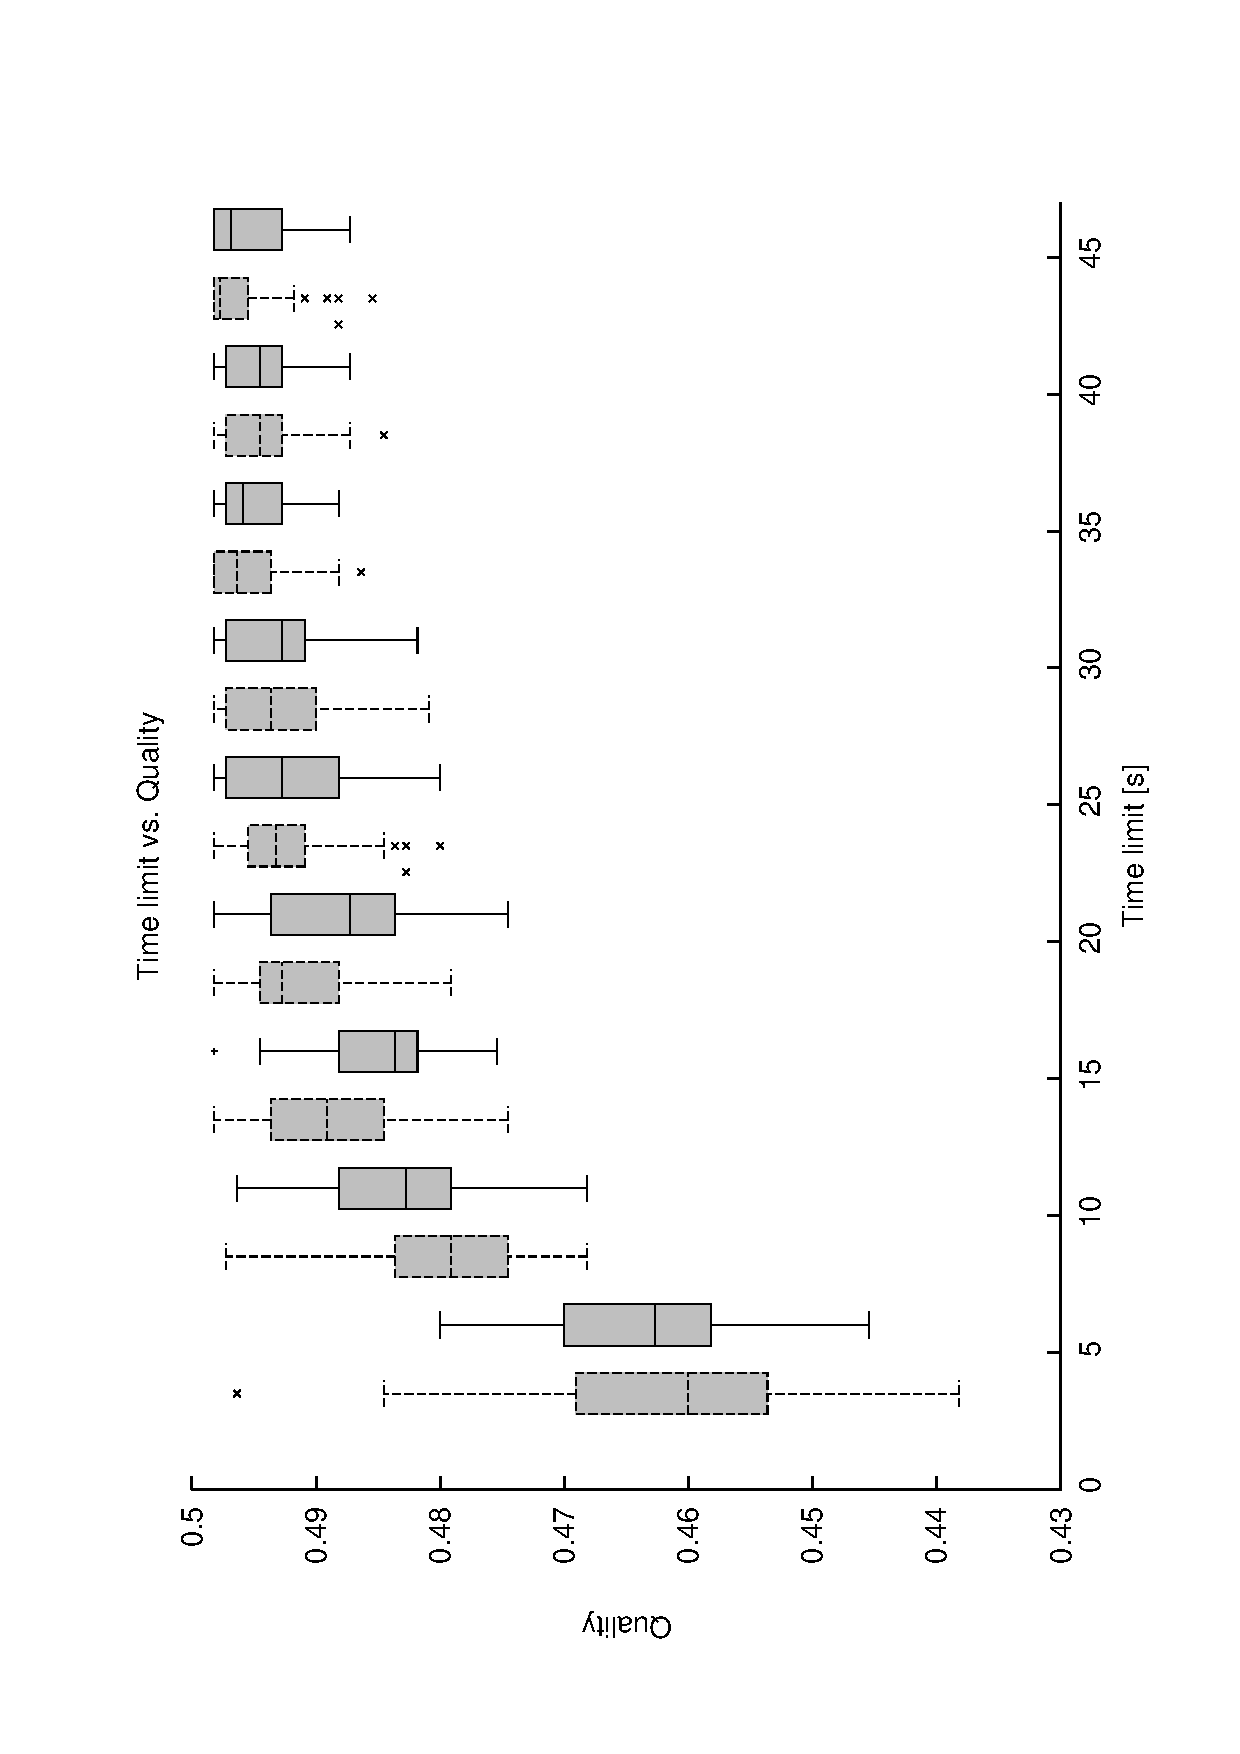
\includegraphics[width=\textwidth]{images/experiments/time-vs-quality}
\end{figure}

Results are in Figure \ref{image-experiment-time-vs-quality}. They should be interpreted as follows: for each time limit from 1 to 46 seconds there are two boxplots next to each other, the left, dashed one is the native GLPK, the right, solid one is the Cygwin GLPK. This is reflected in the tics on the X (time) axis, meaning that the axis cannot be interpreted in the usual way.

We can see from the graph that even though for smaller times (1 and 6 seconds, respectively) the Cygwin GLPK is reaching better qualities with smaller variance, starting from 11 seconds the native GLPK is at least as good or better for every following time. The results are inconclusive though, it is necessary to wait for confirmation from the second part of this experiment.

\begin{center}
\bigskip
\begin{tabular}{| l | l |}
  \hline
  \hline
  Input data        & all sized test data sets \\
  Iterations        & 50 \\
  Pool size         & 1 \\
  $\alpha$, $\beta$ & $1$, $1$ \\
  CH                & \heu{Glpk} \\
  IHs               & $\emptyset$ \\
  \hline
\end{tabular}
\bigskip
\end{center}

The other way to compare the performance of these two GLPK versions is to see how long it takes them to find the optimum for a set of data of increasing size. This experimental set will contain 550 configurations for each version. Every configuration will let \heu{Glpk} CH run for unlimited time, until it finds the optimum. This will be repeated in 50 iterations for each of the 11 files from the sized test data set (see Listing \ref{listing-experiment-glpk-native-vs-cygwin-2}). There will again be no IH, the only data we will collect are the times of the CH run in each case.\\

\begin{algorithm}
\caption{GLPK: native vs. Cygwin set generation 2}
\label{listing-experiment-glpk-native-vs-cygwin-2}
\begin{algorithmic}
\ENSURE experimental set $ES$
\STATE $ES \gets \emptyset$
\FOR{$i = 1 \to 50$}
	\FOR{$file \in $ sized test data}
    \STATE $ES \gets ES \cup \{file, CH = \heu{Glpk}(no\:limit), IH = \emptyset\}$
  \ENDFOR
\ENDFOR
\RETURN $ES$
\end{algorithmic}
\end{algorithm}

\begin{figure}
  \caption{Time Until Optimum}
  \label{image-experiment-time-until-optimum}
  \centering
    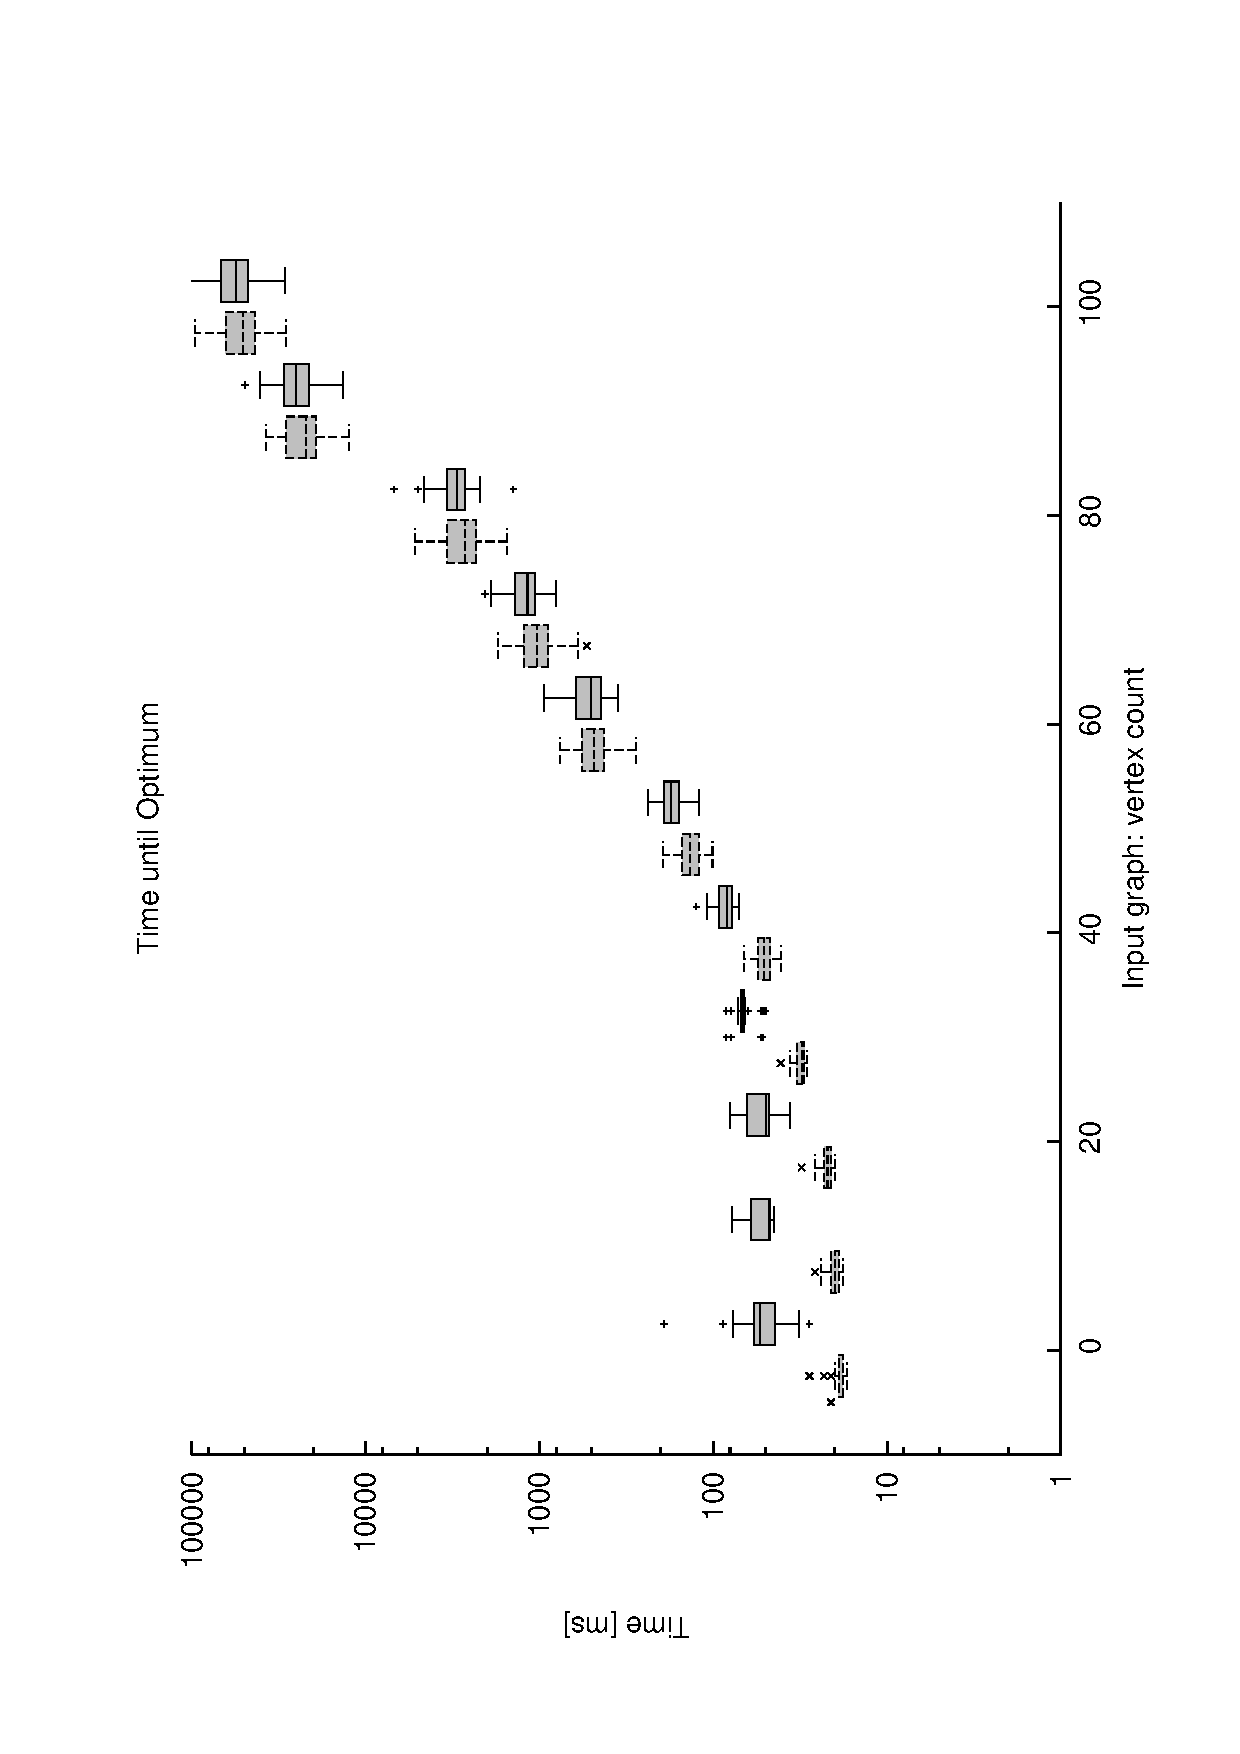
\includegraphics[width=\textwidth]{images/experiments/time-till-optimum}
\end{figure}

Results are in Figure \ref{image-experiment-time-until-optimum}, please take a note that the Y axis is in log scale. As with the previous case, the X axis cannot be interpreted in the usual way. For each data set there are two boxplots next to each other: the left one is the native GLPK, the right one is the Cygwin GLPK.

From these results it becomes clear that the native GLPK has in general shorter running times for each and every input data set than its Cygwin counterpart. This becomes less extreme with the increasing input size, which leads us to suspicion that the core parts of computation in both cases are equally powerful. Regardless of that, we shall be using the \textbf{native} GLPK for following experiments.

To conclude the first timing experiments we introduce a summary pie chart in Figure \ref{image-experiment-timing-summary}. This shows the typical distribution of times needed to find the optimum for the \dataset{OVA3} data set.

These experiments proved that for bigger data sets the times to reach the optimum might become too long. We shall attempt to find heuristics to reach the optimum faster in the following experiments.

% TODO fix this chart
\begin{figure}
  \caption{Timing Summary}
  \label{image-experiment-timing-summary}
  \centering
    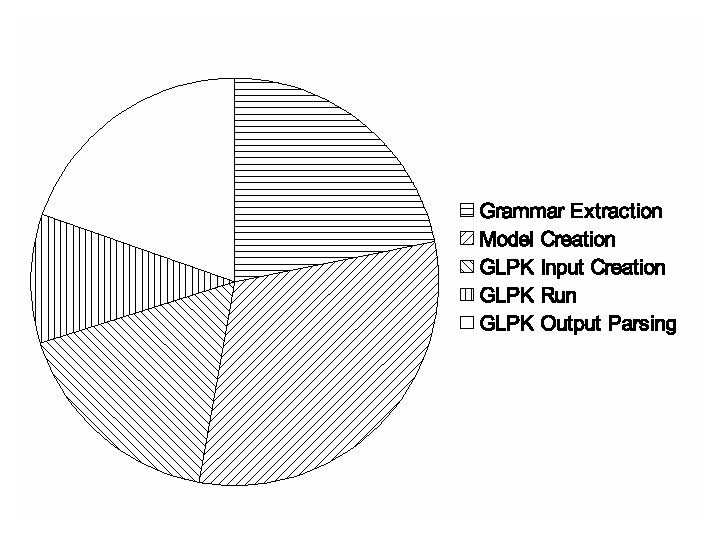
\includegraphics[width=.6\textwidth]{images/experiments/timing-pie}
\end{figure}

\subsection{\heu{Random} vs. \heu{Fuzzy} vs. \heu{FIDAX}}
\label{section-experiments-random-fuzzy-fidax}

%         NB class RandomVsFuzzyVsFidaxStart

Our investigation into various CHs will start by comparing \heu{FIDAX} from the original article \cite{fidax} to 2 of our trivial randomized hungry heuristics, \heu{Random} and \heu{Fuzzy}.

\begin{center}
\bigskip
\begin{tabular}{| l | l |}
  \hline
  \hline
  Input data set    & all official test data sets \\
  Iterations        & 50 \\
  Pool size         & 10 \\
  $\alpha$, $\beta$ & $1$, $1$ \\
  CH                & \heu{Random}, \heu{Fuzzy}, \heu{FIDAX} \\
  IHs               & $\emptyset$ \\
  \hline
\end{tabular}
\bigskip
\end{center}

The experimental set will contain 1650 configurations in total: 3 different CHs * 11 official test data sets * 50 iterations. There will be no improvement heuristics. The pool size will be set to 10, even though \heu{FIDAX} cannot not profit from this. Listing for this can be found in \ref{listing-experiment-random-fuzzy-fidax}.

We will be gathering the running time of the CH itself and quality of the best solution found for GnuPlot.\\

\begin{algorithm}
\caption{\heu{Random} vs. \heu{Fuzzy} vs. \heu{FIDAX} Set Generation}
\label{listing-experiment-random-fuzzy-fidax}
\begin{algorithmic}
\ENSURE experimental set $ES$
\STATE $ES \gets \emptyset$
\FOR{$i = 1 \to 50$}
	\FOR{$file \in $ official test data}
    \STATE $ES \gets ES \cup \{file, CH = \heu{Random}(pool = 10), IH = \emptyset\} \cup \{file, CH = \heu{Fuzzy}(pool = 10), IH = \emptyset\} \cup \{file, CH = \heu{FIDAX}, IH = \emptyset\}$
  \ENDFOR
\ENDFOR
\RETURN $ES$
\end{algorithmic}
\end{algorithm}

\begin{figure}
  \caption{Random vs. Fuzzy vs. FIDAX - Quality}
  \label{image-experiment-random-fuzzy-fidax-quality}
  \centering
    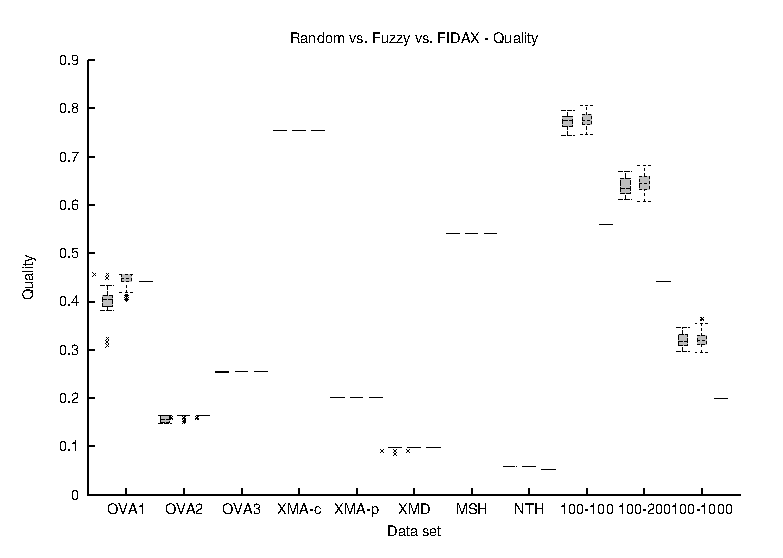
\includegraphics[width=\textwidth]{images/experiments/random-fuzzy-fidax-quality}
\end{figure}

\begin{figure}
  \caption{Random vs. Fuzzy vs. FIDAX - Time}
  \label{image-experiment-random-fuzzy-fidax-time}
  \centering
    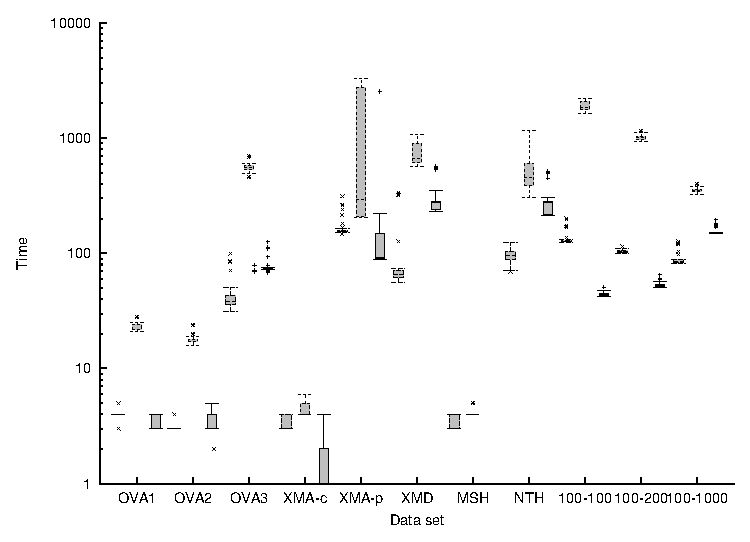
\includegraphics[width=\textwidth]{images/experiments/random-fuzzy-fidax-time}
\end{figure}

Results can be found in Figure \ref{image-experiment-random-fuzzy-fidax-quality} - qualities achieved and Figure \ref{image-experiment-random-fuzzy-fidax-time} - times spent. The Y (time) axis in the latter figure is again in log scale. For each data set there are 3 boxplots next to each other. The first, leftmost, represents \heu{Random}, second \heu{Fuzzy} and finally the third, rightmost is \heu{FIDAX}.

We can draw the following conclusions. \heu{Fuzzy} consistently finds the best solution, but it's by far the slowest of these CHs. The trivial \heu{Random} is better than \heu{FIDAX} in artificial as well as some real data.

\subsubsection{Improving \heu{FIDAX} with \heu{Hungry}}

%         NB class FidaxWithHungry

Now we shall try to answer a minor question, whether it is possible to improve \heu{FIDAX} by using \heu{Hungry} as IH. This short experiment answers that question.

\begin{center}
\bigskip
\begin{tabular}{| l | l |}
  \hline
  \hline
  Input data set    & all official test data sets \\
  Iterations        & 1 \\
  Pool size         & 1 \\
  $\alpha$, $\beta$ & $1$, $1$ \\
  CH                & \heu{FIDAX} \\
  IHs               & \heu{Hungry} or $\emptyset$ \\
  \hline
\end{tabular}
\bigskip
\end{center}

We need a pool size of one and only a single iteration - both \heu{FIDAX} and \heu{Hungry} are deterministic. We will try all official data sets, first with empty IH, second with \heu{Hungry} as IH. We will gather the qualities in each case and see whether there is any improvement.\\

The experimental results are summarized in the Table \ref{table-experiments-fidax-and-hungry} and are quite surprising. As trivial a heuristic \heu{Hungry} is, it is still able to improve the ID set found by \heu{FIDAX} by as much as almost 50\% (the last row, \dataset{100-1000}).

Table \ref{table-experiments-fidax-and-hungry-idsets} lists the ID attributes found in both cases for this most extreme input, \dataset{100-1000}. Note that the content of each cell means ``attribute \texttt{attr} in element \texttt{vertexXY} should be marked as ID attribute".

\begin{table}
  \caption{Results of adding \heu{Hungry} after \heu{FIDAX}}
  \bigskip
  \label{table-experiments-fidax-and-hungry}
  \centering
  \begin{tabular}{l | l | l}
    Data set & Quality - \heu{FIDAX} & Quality - \heu{FIDAX} + \heu{Hungry} \\
    \hline
    \dataset{OVA1}     & 0.4411764705882353  & 0.4411764705882353   \\
    \dataset{OVA2}     & 0.16346153846153846 & 0.16346153846153846  \\
    \dataset{OVA3}     & 0.25482414123443264 & \textbf{0.2553715615163541}   \\
    \dataset{XMA-c}    & 0.7546666666666666	 & 0.7546666666666666   \\
    \dataset{XMA-p}    & 0.2019306150568969	 & 0.2019306150568969   \\
    \dataset{XMD}      & 0.09786094165493509 & 0.09786094165493509  \\
    \dataset{MSH}      & 0.5416472778036296	 & 0.5416472778036296   \\
    \dataset{NTH}      & 0.05259709474828076 & \textbf{0.057918595422124436} \\
    \dataset{100-100}  & 0.56	               & \textbf{0.6766666666666669}   \\
    \dataset{100-200}  & 0.44200000000000017 & \textbf{0.5980000000000003}   \\
    \dataset{100-1000} & 0.19952380952380955 & \textbf{0.29619047619047617}  \\
  \end{tabular}
\end{table}

% TODO for some reason \texttt{\textbf{vertex5}} looks only like \texttt{vertex5}
\begin{table}
  \caption{ID Sets in \heu{FIDAX} Versus \heu{FIDAX} + \heu{Hungry}}
  \bigskip
  \label{table-experiments-fidax-and-hungry-idsets}
  \centering
  \begin{tabular}{l | l}
  \heu{FIDAX} & \heu{FIDAX} + \heu{Hungry} \\
  \hline
                    & \texttt{\textbf{vertex5}}  \\
                    & \texttt{\textbf{vertex26}} \\
  \texttt{vertex30} & \texttt{vertex30} \\
  \texttt{vertex31} & \texttt{vertex31} \\
  \texttt{vertex32} & \texttt{vertex32} \\
  \texttt{vertex34} & \texttt{vertex34} \\
  \texttt{vertex35} & \texttt{vertex35} \\
  \texttt{vertex36} & \texttt{vertex36} \\
  \texttt{vertex37} & \texttt{vertex37} \\
  \texttt{vertex39} & \texttt{vertex39} \\
                    & \texttt{\textbf{vertex60}} \\
                    & \texttt{\textbf{vertex69}} \\
                    & \texttt{\textbf{vertex70}} \\
  \texttt{vertex74} & \texttt{vertex74} \\
  \texttt{vertex75} & \texttt{vertex75} \\
  \texttt{vertex80} & \texttt{vertex80} \\
  \end{tabular}
\end{table}

\subsection{Best Standalone CH}

%         NB class BestStandaloneCH

% TODO re-run on Dual Core!

We shall now try to find the best standalone CH, that is the CH that finds on average the best solutions when run without any IHs. We need to set a time limit for \heu{Glpk} to make it an instance of \heu{Truncated Branch \& Bound}, and we shall use 1 second. This is the smallest time limit possible for GLPK and it is still a reasonably short time, fair to other CHs.

\begin{center}
\bigskip
\begin{tabular}{| l | l |}
  \hline
  \hline
  Input data        & all official test data sets \\
  Iterations        & 50 \\
  Pool size         & 10 \\
  $\alpha$, $\beta$ & $1$, $1$ \\
  CH                & various \\
  IHs               & $\emptyset$ \\
  \hline
\end{tabular}
\bigskip
\end{center}

We will use all the official data sets, set the pool size to 10 where applicable, $\alpha$ and $\beta$ to 1. This experiment will consist of 50 iterations * 11 data sets * 6 CHs = 3300 experimental configurations. See the Listing \ref{listing-experiment-best-standalone-ch} for details. This time we are not interested in run times, only in qualities which we shall gather in a format for GnuPlot.\\

\begin{algorithm}
\caption{Best Standalone CH Set Generation}
\label{listing-experiment-best-standalone-ch}
\begin{algorithmic}
\ENSURE experimental set $ES$
\STATE $ES \gets \emptyset$
\FOR{$file \in $ official test data}
	\FOR{$i = 1 \to 50$}
    	\STATE $ES \gets ES \cup \{file, CH = \heu{Random}, IH = \emptyset\}$
    	\STATE $ES \gets ES \cup \{file, CH = \heu{Fuzzy}, IH = \emptyset\}$
    	\STATE $ES \gets ES \cup \{file, CH = \heu{Incremental}, IH = \emptyset\}$
    	\STATE $ES \gets ES \cup \{file, CH = \heu{Removal}, IH = \emptyset\}$
    	\STATE $ES \gets ES \cup \{file, CH = \heu{FIDAX}, IH = \emptyset\}$
    	\STATE $ES \gets ES \cup \{file, CH = \heu{Glpk}(limit = 1), IH = \emptyset\}$
  \ENDFOR
\ENDFOR
\RETURN $ES$
\end{algorithmic}
\end{algorithm}

For data sets \heu{XMA-c}, \heu{XMA-p}, \heu{MSH} and \heu{NTH} every CH found the optimum every time. Graphs representing the results for remaining data sets can be found in Figure \ref{image-experiments-best-standalone-ch}.

\begin{figure}
  \caption{Best Standalone CH}
  \label{image-experiments-best-standalone-ch}
  \centering
  	\subfigure[\dataset{OVA1}]{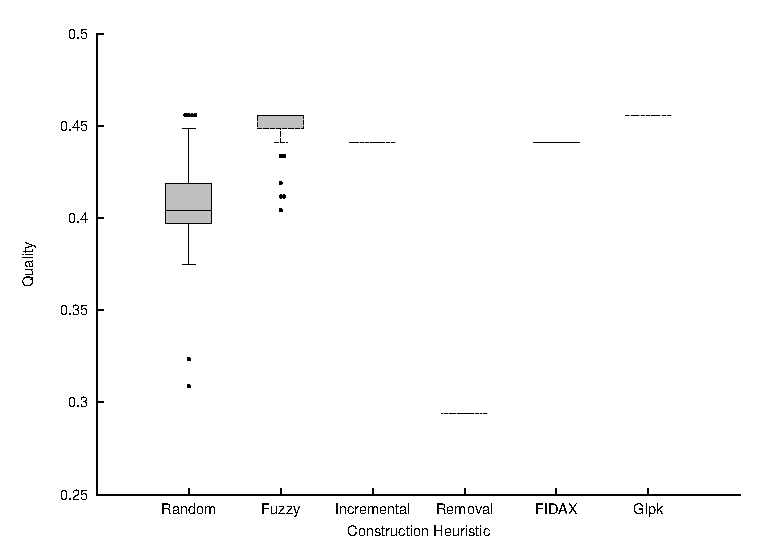
\includegraphics[width=.45\textwidth]{images/experiments/best-ch-OVA1}}
  	\subfigure[\dataset{OVA2}]{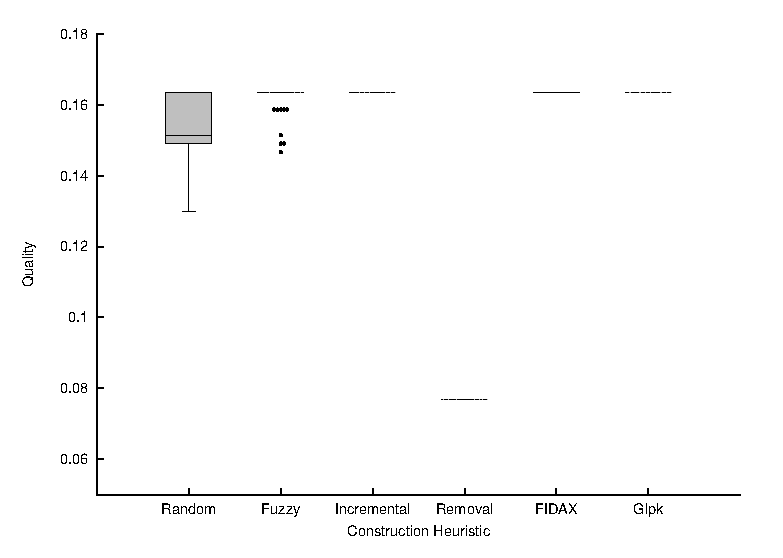
\includegraphics[width=.45\textwidth]{images/experiments/best-ch-OVA2}}
  	\subfigure[\dataset{OVA3}]{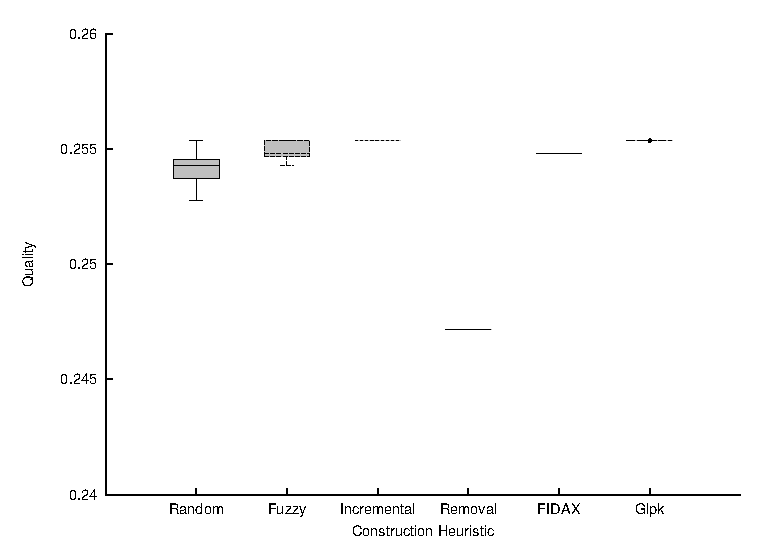
\includegraphics[width=.45\textwidth]{images/experiments/best-ch-OVA3}}
  	\subfigure[\dataset{XMD}]{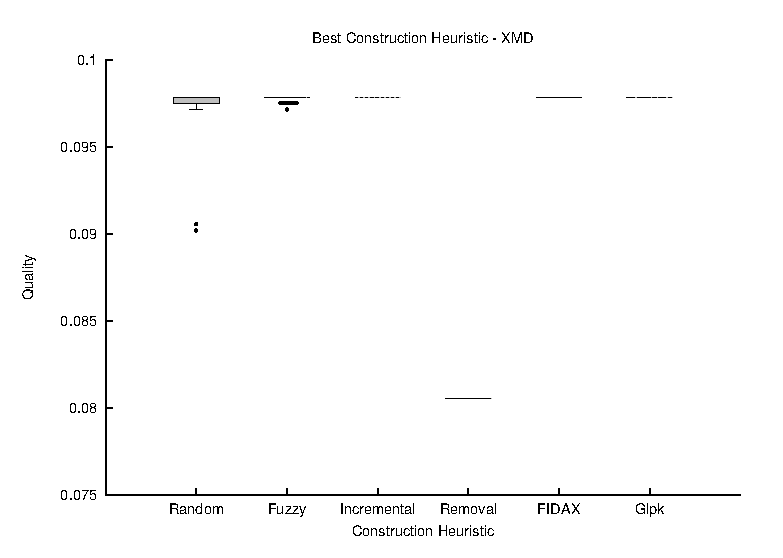
\includegraphics[width=.45\textwidth]{images/experiments/best-ch-XMD}}
   	\subfigure[\dataset{100-100}]{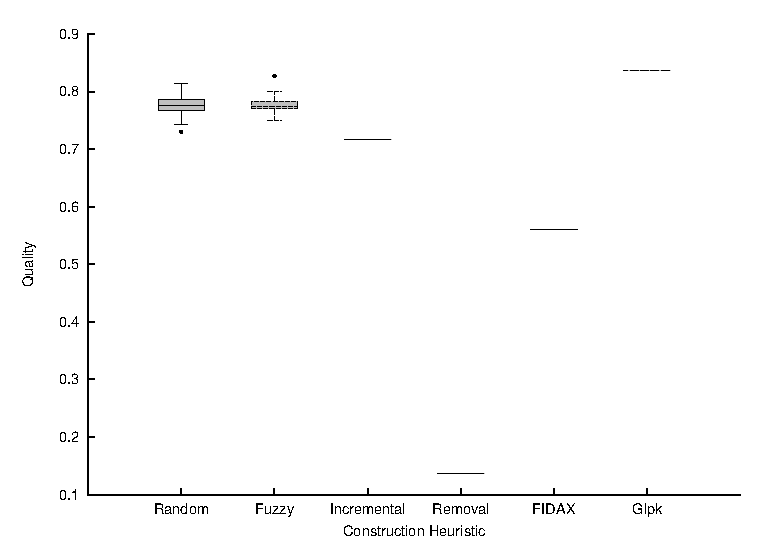
\includegraphics[width=.45\textwidth]{images/experiments/best-ch-100-100}}
  	\subfigure[\dataset{100-200}]{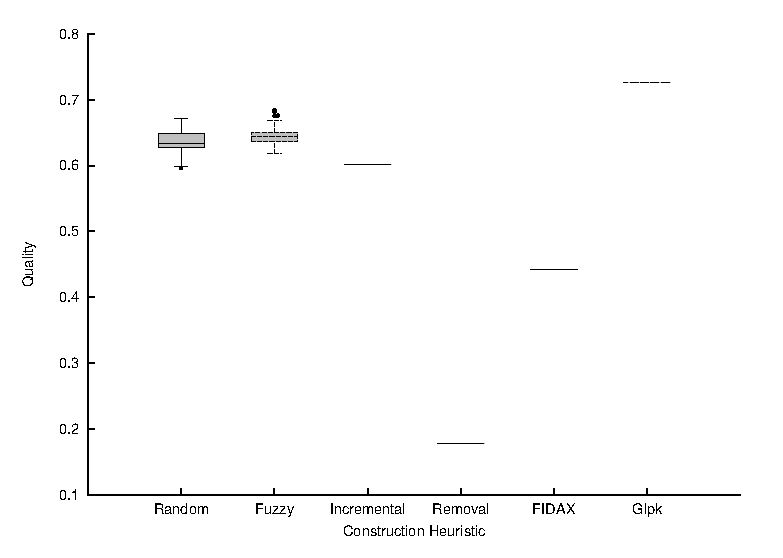
\includegraphics[width=.45\textwidth]{images/experiments/best-ch-100-200}}
  	\subfigure[\dataset{100-1000}]{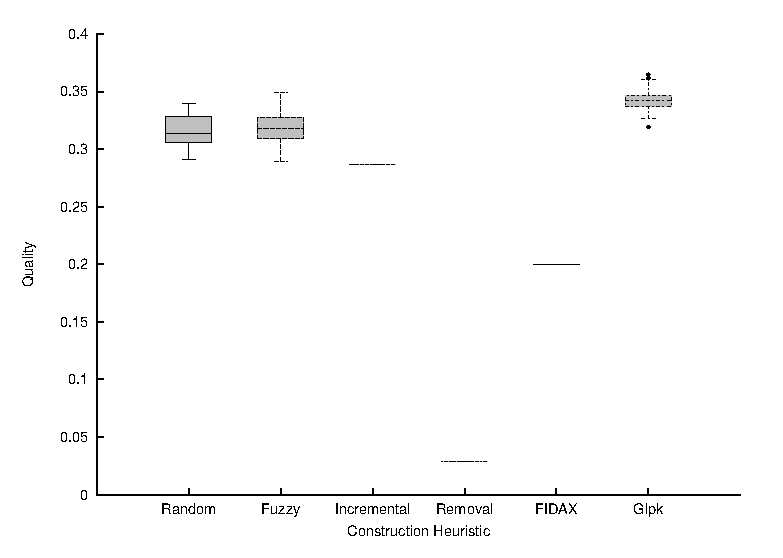
\includegraphics[width=.45\textwidth]{images/experiments/best-ch-100-1000}}
\end{figure}

We can see that \heu{Glpk} wins in every single case. We will start from there and try to build upon this result.

\subsection{Best IH for \heu{Glpk}}

%         NB class BestIHForGlpk

The next logical step will be to try to add one IH after the best CH we have found, \heu{Glpk}. We will investigate all IHs except for \heu{RandomRemove} and \heu{RemoveWorst}, which cannot help us at this time.

We should note that the combination \textit{best CH - best IH} found this way does not necessarily need to be the best one overall, because we find it using a hungry approach.

\begin{center}
\bigskip
\begin{tabular}{| l | l |}
  \hline
  \hline
  Input data        & \dataset{80-30}, \dataset{90-405}, \dataset{100-500}, \\
                    & \dataset{100-100}, \dataset{100-200}, \dataset{100-1000} \\
  Iterations        & 50 \\
  Pool size         & 10 \\
  $\alpha$, $\beta$ & $1$, $1$ \\
  CH                & \heu{Glpk} \\
  IHs               & \heu{Crossover}, \heu{Hungry}, \heu{Local Branching}, \heu{Mutation} \\
  \hline
\end{tabular}
\bigskip
\end{center}

This experimental set will contain 6 data sets * 50 iterations * 4 IHs = 1200 experimental configurations. Note that we are using only the most challenging data sets, as the combination of \heu{Glpk} as CH and any other IH is already an overkill for easier data sets.\\

\begin{algorithm}
\caption{Best IH for \heu{Glpk} Set Generation}
\label{listing-experiment-best-ih-for-glpk}
\begin{algorithmic}
\ENSURE experimental set $ES$
\STATE $ES \gets \emptyset$
\FOR{$file \in \{\dataset{80-30}, \dataset{90-405}, \dataset{100-500}, \dataset{100-100}, \dataset{100-200}, \dataset{100-1000}\}$}
	\FOR{$i = 1 \to 50$}
    	\STATE $ES \gets ES \cup \{file, CH = \heu{Glpk}(limit = 1), IH = \heu{Crossover}(ratio = 0.1, limit = 1)\}$
    	\STATE $ES \gets ES \cup \{file, CH = \heu{Glpk}(limit = 1), IH = \heu{Hungry}\}$
    	\STATE $ES \gets ES \cup \{file, CH = \heu{Glpk}(limit = 1), IH = \heu{Local Branching}(ratio = 0.1, limit = 1)\}$
    	\STATE $ES \gets ES \cup \{file, CH = \heu{Glpk}(limit = 1), IH = \heu{Mutation}(ratio = 0.1, limit = 1)\}$
  \ENDFOR
\ENDFOR
\RETURN $ES$
\end{algorithmic}
\end{algorithm}

The results are listed in Table \ref{table-experiments-best-ih-for-glpk}. We shall denote \textit{improvement} the absolute increase in quality after running \heu{Glpk} and after running the IH. The table now lists for each data set and each IH the average improvement as well as the standard deviation of the improvement. Bold number represents the best IH for that specific data set. \heu{Mutation} proves to be the best IH for 3 out of 6 data sets.

\begin{table}
  \caption{Best IH for \heu{Glpk}}
  \bigskip
  \label{table-experiments-best-ih-for-glpk}
  \centering
  \begin{tabular}{l || l | l || l | l}
             & \heu{Hungry} & \heu{Hungry} & \heu{Crossover} & \heu{Crossover} \\
    Data set & improv - avg & improv - stdev & improv - avg & improv - stdev \\
    \hline
    \dataset{80-320} & 0.00017 & 0.00118 & 0.00017 & 0.00118 \\
    \dataset{90-405} & 0.00502 & 0.00618 & 0.00033 & 0.00165 \\
    \dataset{100-500} & 0.00664 & 0.00667 & 0.00016 & 0.00081 \\
    \hline
    \dataset{100-100} & 0.00000 & 0.00000 & 0.00000 & 0.00000 \\
    \dataset{100-200} & 0.00000 & 0.00000 & 0.00000 & 0.00000 \\
    \dataset{100-1000} & 0.01630 & 0.01294 & 0.00180 & 0.00506 \\
  \end{tabular}    
	% TODO separate somehow
  \begin{tabular}{l || l | l || l | l}
             & \heu{LB} & \heu{LB} & \heu{Mutation} & \heu{Mutation} \\
    Data set & improv - avg & improv - stdev & improv - avg & improv - stdev \\
    \hline
    \dataset{80-320} & \textbf{0.00072} & 0.00223 & 0.00064 & 0.00218 \\
    \dataset{90-405} & 0.00698 & 0.00616 & \textbf{0.00851} & 0.00659 \\
    \dataset{100-500} & 0.00796 & 0.00797 & \textbf{0.00964} & 0.00804 \\
    \hline
    \dataset{100-100} & 0.00000 & 0.00000 & 0.00000 & 0.00000 \\
    \dataset{100-200} & 0.00000 & 0.00000 & 0.00000 & 0.00000 \\
    \dataset{100-1000} & 0.01710 & 0.01188 & \textbf{0.02337} & 0.01558 \\
  \end{tabular}
\end{table}

\subsubsection{\heu{Random} as CH}

%         NB class CHForMutation

As we mentioned before, we chose the combination \heu{Glpk} and \heu{Mutation} in a hungry manner. We will now try to take a step back and attempt to replace \heu{Glpk} with \heu{Random}, hoping to get similar qualities in much shorter time (a reminder: \heu{Glpk} always takes 1 second).

\begin{center}
\bigskip
\begin{tabular}{| l | l |}
  \hline
  \hline
  Input data        & \dataset{80-30}, \dataset{90-405}, \dataset{100-500}, \\
                    & \dataset{100-100}, \dataset{100-200}, \dataset{100-1000} \\
  Iterations        & 50 \\
  Pool size         & 10 \\
  $\alpha$, $\beta$ & $1$, $1$ \\
  CH                & \heu{Random} or \heu{Glpk} \\
  IHs               & \heu{Mutation} \\
  \hline
\end{tabular}
\bigskip
\end{center}

Setup used will be almost identical to that from the previous experiment. Experimental set will consist of 6 data sets * 50 iterations * 2 CHs = 600 experimental configurations, see Listing \ref{listing-experiment-ch-for-mutation}. We shall collect the eventual quality after running both the CH and the IH in format suited for GnuPlot.\\

\begin{algorithm}
\caption{\heu{Random} as CH Set Generation}
\label{listing-experiment-ch-for-mutation}
\begin{algorithmic}
\ENSURE experimental set $ES$
\STATE $ES \gets \emptyset$
\FOR{$file \in \{\dataset{80-30}, \dataset{90-405}, \dataset{100-500}, \dataset{100-100}, \dataset{100-200}, \dataset{100-1000}\}$}
	\FOR{$i = 1 \to 50$}
    	\STATE $ES \gets ES \cup \{file, CH = \heu{Random}, IH = \heu{Mutation}(ratio = 0.1, limit = 1)\}$
    	\STATE $ES \gets ES \cup \{file, CH = \heu{Glpk}(limit = 1), IH = \heu{Mutation}(ratio = 0.1, limit = 1)\}$
  \ENDFOR
\ENDFOR
\RETURN $ES$
\end{algorithmic}
\end{algorithm}

Results are summarized in Figure \ref{image-experiment-ch-for-mutation}. Again, for each data set there are two boxplots representing \heu{Random} (left one) and \heu{Glpk} (right one). The combination \heu{Glpk} + \heu{Mutation} always finds the optimum for the simpler data sets, thus the collapsed boxplots. Moreover, it achieves higher quality in each data set. On the other hand, combination \heu{Random} + \heu{Mutation} has much shorter running times and in the biggest (and hardest) data set \dataset{100-1000} has almost comparable results. This makes it a reasonable choice for big inputs where short time is more important than optimal quality.

\begin{figure}
  \caption{CH for \heu{Mutation}}
  \label{image-experiment-ch-for-mutation}
  \centering
    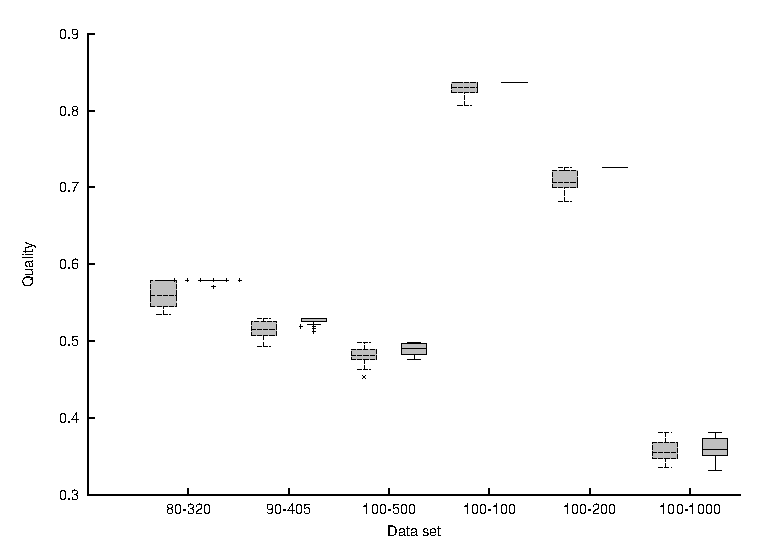
\includegraphics[width=\textwidth]{images/experiments/ch-for-mutation}
\end{figure}

% TODO this subsection does not play well with the ToC - how to put something else in the ToC than is here?
\subsection{Various $\alpha$, $\beta$}

After finding the best combination of a CH and IH we turn our attention to some of the parameters. The first ones are the $\alpha$ and $\beta$ from the definition of our weight function. % TODO link
A short reminder: the weight is defined as TODO copy formula. It is thus obvious that only the \textit{ratio} between $\alpha$ and $\beta$ matters, not their actual values. This means that investigating effects of these parameters is in fact a 1-dimensional problem. However, for simplicity's sake we will use 25 combinations of various $\alpha$ and $\beta$ and normalize them only during evaluation.

It is worthy noting that we do not expect any changes in performance of heuristics and we will limit the inquiry to different ID sets produced under different settings.

\begin{center}
\bigskip
\begin{tabular}{| l | l |}
  \hline
  \hline
  Input data        & realistic + converted official test data sets \\
  Iterations        & 1 \\
  Pool size         & 1 \\
  $\alpha$, $\beta$ & $\{0.1, 0.25, 0.5, 0.75, 1\} \times \{0.1, 0.25, 0.5, 0.75, 1\}$ \\ % TODO this is not the best way to write it
  CH                & \heu{Glpk} \\
  IHs               & $\emptyset$ \\
  \hline
\end{tabular}
\bigskip
\end{center}

This experimental set will contain 5 different $\alpha$ settings * 5 $\beta$ settings * 8 data sets = 200 experimental configurations. We are not using the artificial data sets, because the way they are generated (attribute values are random numbers) they cannot possibly create different optimal ID sets. The pseudocode capturing this is in Listing \ref{listing-experiment-various-betas}. We will use \heu{Glpk} constrained to 1 second (thus making it an instance of \heu{Truncated Branch \& Bound}) and no IHs. Pool size as well as iteration count will be 1. We are noting the actual ID set found by the run of the heuristic.\\

\begin{algorithm}
\caption{Various Values of $\alpha$ and $\beta$ Set Generation}
\label{listing-experiment-various-betas}
\begin{algorithmic}
\ENSURE experimental set $ES$
\STATE $ES \gets \emptyset$
\FOR{$\alpha \in \{0.1, 0.25, 0.5, 0.75, 1\}$}
  \FOR{$\beta \in \{0.1, 0.25, 0.5, 0.75, 1\}$}
    \FOR{$file \in $ realistic of converted official test data}
    	\STATE $ES \gets ES \cup \{file, CH = \heu{Glpk}(limit = 1, alpha = \alpha, beta = \beta), IH = \emptyset\}$
    \ENDFOR
  \ENDFOR
\ENDFOR
\RETURN $ES$
\end{algorithmic}
\end{algorithm}

Following data sets have the same optimal ID sets regardless of the setting of $\alpha$ and $\beta$: \dataset{MSH}, \dataset{NTH}, \dataset{XMA-c}, \dataset{XMA-p}. The \dataset{OVA*} data sets showed various dependencies on $\alpha$ and $\beta$, we shall now describe one representative example.

\subsubsection{Results for \dataset{OVA1}}

The 2 different ID sets found for various $\alpha$ and $\beta$ in \dataset{OVA1} are listed in Table \ref{table-experiments-various-betas-ova1} (note that the actual names had to be anonymized for reasons discussed in Section \ref{section-realistic-data}). The differing attribute mapping is highlited.

\begin{table}
  \caption{Different ID Sets Found for \dataset{OVA1}}
  \bigskip
  \label{table-experiments-various-betas-ova1}
  \centering
  \begin{tabular}{c || c}
    ID set \textbf{1}: element@attribute & ID set \textbf{2}: element@attribute \\
    \hline
    \texttt{aff@fa} & \texttt{aff@fa} \\
    \texttt{com@ty} & \texttt{com@ty} \\
    \texttt{cre@da} & \texttt{cre@da} \\
    \texttt{cri@te} & \texttt{cri@te} \\
    \texttt{cve@st} & \texttt{cve@st} \\
    \texttt{\textbf{def@id}} & \texttt{\textbf{def@cl}} <- \\ % TODO again, my bold typewriter does not work
    \texttt{fil@co} & \texttt{fil@co} \\
    \texttt{mod@da} & \texttt{mod@da} \\
    \texttt{ova@xs} & \texttt{ova@xs} \\
    \texttt{pat@op} & \texttt{pat@op} \\
    \texttt{sof@op} & \texttt{sof@op} \\
    \texttt{sta@da} & \texttt{sta@da} \\
    \texttt{sub@or} & \texttt{sub@or} \\
    \texttt{sbt@te} & \texttt{sbt@te} \\
  \end{tabular}
\end{table}

Table \ref{table-experiments-various-betas-ova1-effect} summarizes the dependency of the ID set found on various values of $\alpha$, $\beta$. We than define the $\alpha-ratio$ as $ \dfrac{\alpha}{\alpha + \beta} $ and summarize the findings in a linear manner, sorted by increasing $\alpha-ratio$ in Table \ref{table-experiments-various-betas-ova1-ratio-effect}. Note that the $\alpha-ratio$s are not unique due to the way we constructed the experimental configurations here.

\begin{table}
  \caption{Effect of $\alpha$, $\beta$ on ID Set Found for \dataset{OVA1}}
  \bigskip
  \label{table-experiments-various-betas-ova1-effect}
  \centering
  \begin{tabular}{c | c  c  c  c  c}
    $\alpha$ \textbackslash $\beta$ & 0.1 & 0.25 & 0.5 & 0.75 & 1 \\
    \hline
    0.1  & 1 & 2 & 2 & 1 & 1 \\
    0.25 & 2 & 2 & 2 & 1 & 2 \\
    0.5  & 2 & 1 & 1 & 1 & 2 \\
    0.75 & 1 & 2 & 1 & 2 & 1 \\
    1    & 1 & 2 & 1 & 1 & 2 \\
  \end{tabular}
\end{table}

\begin{table}
  \caption{Effect of $\alpha-ratio$ on ID Set Found for \dataset{OVA1}}
  \bigskip
  \label{table-experiments-various-betas-ova1-ratio-effect}
  \centering
  \begin{tabular}{c | c || c |  c}
    $\alpha-ratio$ & ID set & $\alpha-ratio$ & ID set \\
    \hline
    0,091	& 1 & 0,500	& 2 \\
    0,118	& 1 & 0,500	& 2 \\
    0,167	& 2 & 0,571	& 1 \\
    0,200	& 2 & 0,600	& 1 \\
    0,250	& 1 & 0,667	& 1 \\
    0,286	& 2 & 0,667	& 1 \\
    0,333	& 2 & 0,714	& 2 \\
    0,333	& 2 & 0,750	& 2 \\
    0,400	& 1 & 0,800	& 2 \\
    0,429	& 1 & 0,833	& 2 \\
    0,500	& 1 & 0,882	& 1 \\
    0,500	& 2 & 0,909	& 1 \\
    0,500	& 1 &       &   \\
  \end{tabular}
\end{table}

Interestingly enough, there is no clear separation between the two ID sets depending on the $\alpha-ratio$ to be found. The very existence of the two sets might be due to the fact that \heu{Glpk} randomizes the order in which AMs are presented to the external GLPK solver. However, this question is outside of the scope of this work, and shall be left for future work.

\subsection{Ignoring Text Data}

%         NB class IgnoreTextData

When considering data sets such as \dataset{XMA-p}, we notice that they contain a lot of simple text nodes that do not contribute to our search, but possibly slow it down. Precisely for this reason the \jmodule{BasicIGG} module in jInfer contains an option to turn off processing of such nodes. (It also allows to ignore the content of attributes, but this would be devastating to our cause.) Ignoring the content of text nodes means internally that these are created, but their actual string content is skipped and not saved in the memory structures. This means that the whole data model occupies less space on the heap, which can possibly lead to better performance.

We shall now investigate this matter by taking the biggest data set \dataset{XMA-p} containing a lot of text data.

\begin{center}
\bigskip
\begin{tabular}{| l | l |}
  \hline
  \hline
  Input data        & \dataset{XMA-p} \\
  Iterations        & 50 \\
  Pool size         & 1 \\
  $\alpha$, $\beta$ & $1$, $1$ \\
  CH                & \heu{Glpk} \\
  IHs               & not applicable \\
  \hline
\end{tabular}
\bigskip
\end{center}

Our experimental set will contain 50 iterations * 2 = 100 experimental configurations as described in Listing \ref{listing-experiment-ignore-text-data}. We will be using \heu{Glpk} limited to 1 second with no additional IH and pool size set to 1. After the first 50 iterations we will turn on the option to ignore the simple text node data and run the same 50 iterations again. We will be collecting the grammar extraction (GE) and model creation (MC) times as in the experiment in Section \ref{section-grammar-model-timing}.\\

\begin{algorithm}
\caption{Ignoring Text Data Set Generation}
\label{listing-experiment-ignore-text-data}
\begin{algorithmic}
\ENSURE experimental set $ES$
\STATE $ES \gets \emptyset$
\FOR{$i \in 1 \to 50 $}
  \STATE $ES \gets ES \cup \{\dataset{XMA-p}, CH = \heu{Glpk}(limit = 1), IH = \emptyset\}$
\ENDFOR
\STATE \textbf{set} ``ignore text data"
\FOR{$i \in 1 \to 50 $}
  \STATE $ES \gets ES \cup \{\dataset{XMA-p}, CH = \heu{Glpk}(limit = 1), IH = \emptyset\}$
\ENDFOR
\RETURN $ES$
\end{algorithmic}
\end{algorithm}

Results are summarized in Figure \ref{image-experiment-ignore-text-data}. Boxplots drawn in dashed lines represent the original case, not ignoring the text data. Solid lines represent the case where we ignore the text data.

Interestingly, the grammar extraction times tend to be shorter in the case when text data is not ignored, although this is inconclusive. However, there is a clear improvement of about 50 \% in the case of model creation times. The conclusion then is to ignore the simple text node content whenever possible when finding ID attributes.

\begin{figure}
  \caption{Ignoring Text Data}
  \label{image-experiment-ignore-text-data}
  \centering
    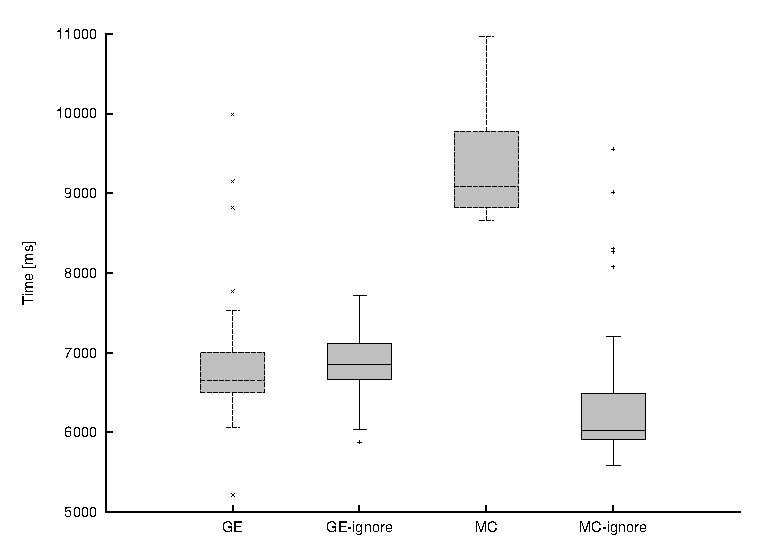
\includegraphics[width=\textwidth]{images/experiments/ignore-text-data}
\end{figure}

\subsection{Chaining the IHs}

%         NB class ChainedIHsX

In this section we will describe the most interesting experimental area, that is chaining more than one improvement heuristics and running them in a loop. Unfortunately, the sheer number of possible combinations in which IHs can be ordered (as well as the number of ways to set their parameters) prohibits us from investigating this in depth.

We shall then employ a higher-level heuristic: we will choose 3 scenarios (lists of IHs, or metaheuristics), assess their performance to find the best one and then tune its parameters. This approach is by no means exhaustive, it is just a probe in the problem space.

The 3 scenarios we will be assessing will be constructed from the following instances of improvement heuristics:

\begin{itemize}
	\item \heu{RR} is \heu{RandomRemove} with $ratio$ set to $0.1$.
	\item \heu{MUT} is \heu{Mutation} with $ratio$ set to $0.1$ and time limit set to 1 second.
	\item \heu{CX} is \heu{Crossover} with $ratio$ set to $0.1$ and time limit set to 1 second.
	\item \heu{LB} is \heu{LocalBranching} with $ratio$ set to $0.1$ and time limit set to 1 second.
	\item \heu{RW} is \heu{RemoveWorst}.
	\item \heu{H} is \heu{Hungry}.
\end{itemize}

The scenarios themselves shall be the following:

\begin{itemize}
	\item \textit{\textbf{Scenario 1}}. \heu{RR} $\rightarrow$ \heu{MUT} $\rightarrow$ \heu{RR} $\rightarrow$ \heu{CX} $\rightarrow$ \heu{RW} $\rightarrow \ldots$
	\item \textit{\textbf{Scenario 2}}. \heu{CX} $\rightarrow$ \heu{RW} $\rightarrow$ \heu{MUT} $\rightarrow \ldots$
	\item \textit{\textbf{Scenario 3}}. \heu{CX} $\rightarrow$ \heu{RR} $\rightarrow$ \heu{MUT} $\rightarrow$ \heu{RW} $\rightarrow$ \heu{LB} $\rightarrow$ \heu{RW} $\rightarrow \ldots$
\end{itemize}

\begin{center}
\bigskip
\begin{tabular}{| l | l |}
  \hline
  \hline
  Input data        & all official test data sets \\
  Iterations        & 20 \\
  Pool size         & 10 \\
  $\alpha$, $\beta$ & $1$, $1$ \\
  CH                & \heu{Random} \\
  IHs               & various \\
  \hline
\end{tabular}
\bigskip
\end{center}

The experimental set will consist of 3 scenarios * 11 data sets * 20 iterations = 660 experimental configurations. Their construction is formalized in the Listing \ref{listing-experiment-chaining-ihs}. The construction heuristic will be \heu{Random} with pool size 10. All the ratios are set to $0.1$ for the time being. The termination criterion is set to limit the total runtime to 10 seconds and (potentialy) infinite iterations.

Data gathered will be traces like the one in Appendix \ref{appendix-trace} - after each iteration, the time taken so far and the quality of incumbent solution is noted.\\

\begin{algorithm}
\caption{Chaining IHs Set Generation}
\label{listing-experiment-chaining-ihs}
\begin{algorithmic}
\ENSURE experimental set $ES$
\STATE $ES \gets \emptyset$
\STATE $\heu{MUT} \gets \heu{Mutation}(ratio = 0.1, limit = 1)$
\STATE $\heu{CX} \gets \heu{Crossover}(ratio = 0.1, limit = 1)$
\STATE $\heu{LB} \gets \heu{LocalBranching}(ratio = 0.1, limit = 1)$
\STATE $\heu{RR} \gets \heu{RandomRemove}(ratio = 0.1)$
\STATE $\heu{H} \gets \heu{Hungry}$
\STATE $\heu{RW} \gets \heu{RemoveWorst}$
\STATE $IHs \gets \emptyset$

\STATE $IHs \gets IHs \cup (\heu{RR}, \heu{MUT}, \heu{RR}, \heu{CX}, \heu{RW})$

\STATE $IHs \gets IHs \cup (\heu{CX}, \heu{RW}, \heu{MUT})$

\STATE $IHs \gets IHs \cup (\heu{CX}, \heu{RR}, \heu{MUT}, \heu{RW}, \heu{LB}, \heu{RW}, \heu{H})$

\FOR{$ih \in IHs$}
  \FOR{$file \in $ official test data}
    \FOR{$i = 1 \to 20$}
      \STATE $ES \gets ES \cup \{file, CH = \heu{Random}, IH = ih, limit = 10 seconds\}$
    \ENDFOR
  \ENDFOR
\ENDFOR
\RETURN $ES$
\end{algorithmic}
\end{algorithm}

Resulting traces for each data set can be summarized in graphs like the one for \heu{100-100} in Figure \ref{image-experiment-chained-ihs-s1}. This one deserves more explanation than usual.

\begin{figure}
  \caption{Chained IHs - \dataset{100-100} Results for Scenario 1}
  \label{image-experiment-chained-ihs-s1}
  \centering
    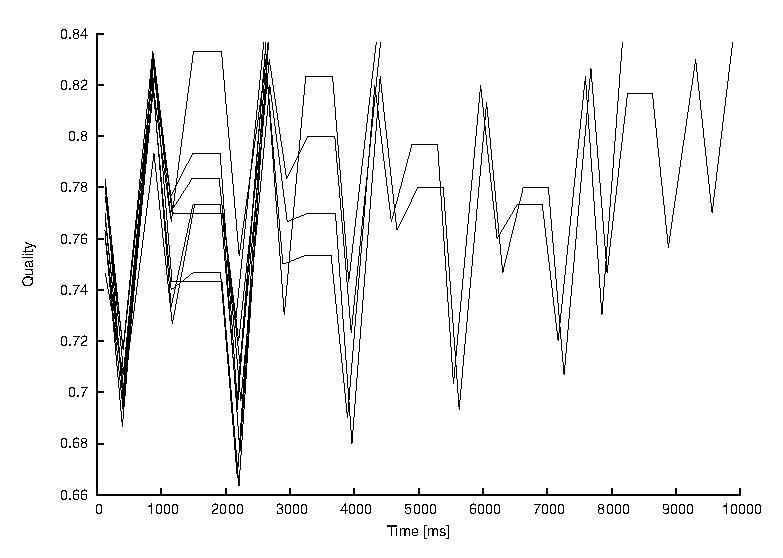
\includegraphics[width=\textwidth]{images/experiments/chained-ihs-s1}
\end{figure}

X and Y axes represent the time and quality, as usual. Each line represents one run of the scenario (metaheuristic) in the following way: the N\textsuperscript{th} break in the line (i.e. the N\textsuperscript{th} data point) is the partial result after the N\textsuperscript{th} step of the scenario. Its X position denotes the absolute time in which this step finished, and its Y position represents the incumbent solution quality after this step. Every time a line disappears before reaching 10 seconds it means that this metaheuristic run found the optimum before the 10 second mark. There is an obvious repetitive regularity in the shape of each line, this corresponds to the fact that there is a finite number of IHs in this scenario (5 of them in Scenario 1) which repeat over time. The obvious similarity between different lines corresponds to the fact that each run is from the same scenario, and over time, they do the same steps. 

We can see effects of different IHs from this graph:
\begin{itemize}
	\item Every $(1 + 5k)$\textsuperscript{th} and $(3 + 5k)$\textsuperscript{th} step is a \heu{RandomRemove}, and each time this happens there is a rather sharp drop in quality
	\item Every $(2 + 5k)$\textsuperscript{th} step is a \heu{Mutation}, and there is a consistent increase in quality each time.
	\item Every $(4 + 5k)$\textsuperscript{th} step is a \heu{Crossover}, and each time it happens there is a consistent increase, yet smaller than with \heu{Mutation}.
	\item Every $5k$\textsuperscript{th} step is a \heu{RemoveWorst}, and as expected, this removes the worst solution not touching the best ones that decide the incumbent quality. The line thus stays flat every time it happens.
\end{itemize}

In this particular example there is only 1 run out of 10 that does not finish (find optimum) under the 10 second mark.\\

There are two more graphs like this in Figures \ref{image-experiment-chained-ihs-s2} and \ref{image-experiment-chained-ihs-s3} for comparison, capturing Scenario 2 and Scenario 3 respectively working on the same data set, \dataset{100-100}. Describing them in detail is unfortunately outside of the scope of this work.\\

\begin{figure}
  \caption{Chained IHs - \dataset{100-100} Results for Scenario 2}
  \label{image-experiment-chained-ihs-s2}
  \centering
    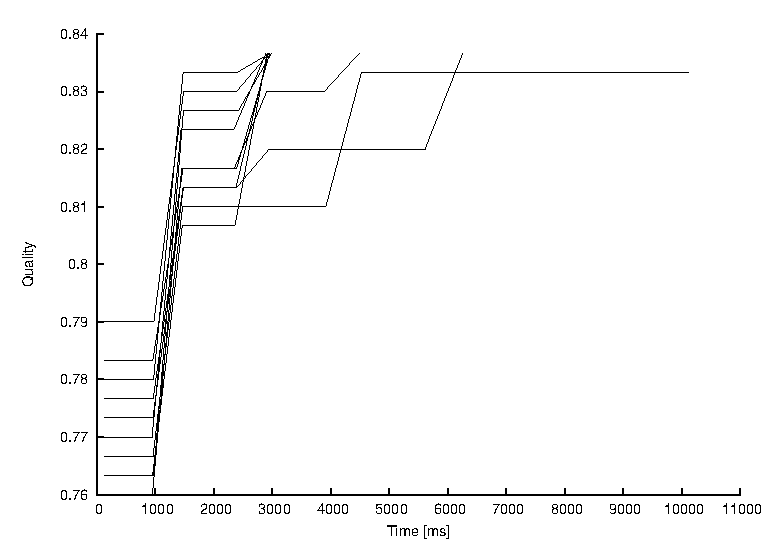
\includegraphics[width=\textwidth]{images/experiments/chained-ihs-s2}
\end{figure}

\begin{figure}
  \caption{Chained IHs - \dataset{100-100} Results for Scenario 3}
  \label{image-experiment-chained-ihs-s3}
  \centering
    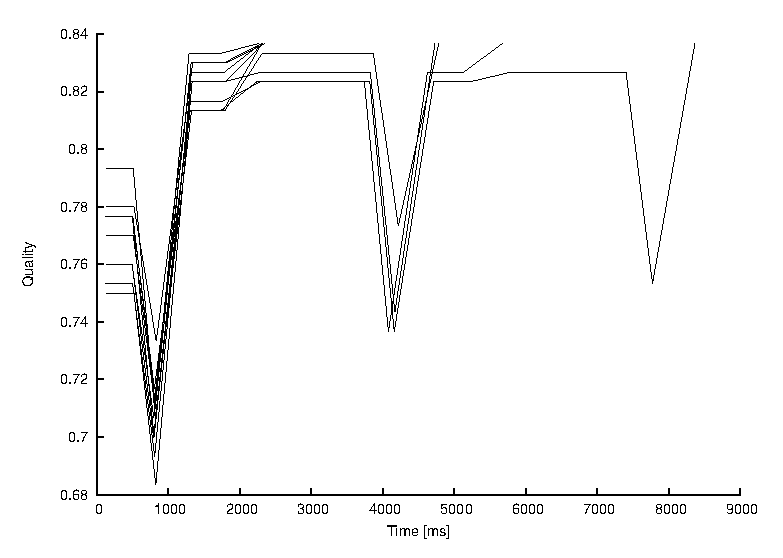
\includegraphics[width=\textwidth]{images/experiments/chained-ihs-s3}
\end{figure}

It is now necessary to assess which of the scenarios perform the best. We shall take a look at the different data sets. Easily we can discard \dataset{MSH}, \dataset{NTH}, \dataset{XMA-c}, \dataset{XMA-p}, because the optimum is found in the very first step. Let us now introduce a metric for assessment of a scenario: namely, how many times of the 20 runs did it find the optimum. Results of this are summarized in Table \ref{table-experiments-chained-ihs-tweaking}.

\begin{table}
  \caption{Performance of Various IH Chains}
  \bigskip
  \label{table-experiments-chained-ihs-tweaking}
  \centering
  \begin{tabular}{l || c | c | c}
    Dataset & Scenario 1 & Scenario 2 & Scenario 3 \\
    \hline
    \dataset{100-100}  & \textbf{20} & 19 & \textbf{20} \\
    \dataset{100-200}  & \textbf{19} & 18 & 17 \\
    \dataset{100-1000} & 4  & 1  & \textbf{5}  \\
    \dataset{OVA1}     & \textbf{20} & \textbf{20} & \textbf{20} \\
    \dataset{OVA2}     & \textbf{19} & 13 & 18 \\
    \dataset{OVA3}     & 17 & 18 & \textbf{20} \\
    \end{tabular}
\end{table}

Each cell contains the number of times the scenario found optimum in the data set, out of 20 runs. Highlited are the scenarios that performed best on that data set. We see that Scenario 1 and 3 are very similar in performance. We shall nonetheless choose Scenario \textbf{1} as the winner for its simplicity. Now we can tune its parameters.

\subsubsection{Improving Scenario 1}

%         NB class ChainedIHs1Tweak

A short reminder: Scenario 1 consists of \heu{Random} as the CH and the following IHs: \heu{RR} $\rightarrow$ \heu{MUT} $\rightarrow$ \heu{RR} $\rightarrow$ \heu{CX} $\rightarrow$ \heu{RW} $\rightarrow \ldots$

The parameters we can tune in this scenario are the ratios in \heu{RandomRemove} (possibly 2 of them, as there are 2 instances in use), \heu{Mutation} and \heu{Crossover}. We shall not tune the time limits in \heu{Mutation} and \heu{Crossover} and leave them set to 1 second. This presents us with a 3-dimensional space of parameters, where we want to find a combination best suited for our test data sets. We will sample this space by taking a total of 45 configurations of the aforementioned ratios.

\begin{center}
\bigskip
\begin{tabular}{| l | l |}
  \hline
  \hline
  Input data        & \dataset{100-100}, \dataset{100-200}, \dataset{100-1000}, \dataset{OVA1}, \dataset{OVA2}, \dataset{OVA3} \\
  Iterations        & 50 \\
  Pool size         & 10 \\
  $\alpha$, $\beta$ & $1$, $1$ \\
  CH                & \heu{Random} \\
  IHs               & \heu{RR} $\rightarrow$ \heu{MUT} $\rightarrow$ \heu{RR} $\rightarrow$ \heu{CX} $\rightarrow$ \heu{RW} $\rightarrow \ldots $ \\
  \hline
\end{tabular}
\bigskip
\end{center}

This experimental set will consist of 45 ratio combinations * 6 data sets * 50 iterations = 13500 experimental configurations. CH will be \heu{Random} with pool size of 10. IHs will be the ones from Scenario 1, with their ratios set to one of the 45 combinations produced in the following way.
\begin{itemize}
	\item \heu{RandomRemove} ratio will be from $\{0, 0.05, 0.1, 0.2, 0.5\}$
	\item \heu{Mutatio} ratio will be from $\{0.05, 0.1, 0.2\}$
	\item \heu{Crossover} ratio will be from $\{0.05, 0.1, 0.2\}$
\end{itemize}
The process of creating the configurations is captured in Listing \ref{listing-experiment-chained-ihs-tuning}. We will be gathering the following information for each run: what were the parameters, how long did the run take and whether it found optimum.\\

\begin{algorithm}
\caption{Chained IHs - Improving Scenario 1 Set Generation}
\label{listing-experiment-chained-ihs-tuning}
\begin{algorithmic}
\ENSURE experimental set $ES$
\STATE $ES \gets \emptyset$

\STATE $RW \gets \heu{RemoveWorst}$

\FOR{$rrRatio \in \{0, 0.05, 0.1, 0.2, 0.5\}$}
\FOR{$mutRatio \in \{0.05, 0.1, 0.2\}$}
\FOR{$cxRatio \in \{0.05, 0.1, 0.2\}$}
  \STATE $RR \gets \heu{RandomRemoval}(ratio = rrRatio)$
  \STATE $MUT \gets \heu{Mutation}(ratio = mutRatio, limit = 1)$
  \STATE $CX \gets \heu{Crossover}(ratio = cxRatio, limit = 1)$
  \FOR{$file \in \{\dataset{100-100}, \dataset{100-200}, \dataset{100-1000}, \dataset{OVA1}, \dataset{OVA2}, \dataset{OVA3}\}$}
    \FOR{$i = 1 \to 50$}
      \STATE $ES \gets ES \cup \{file, CH = \heu{Random}, IH = (\heu{RR}, \heu{MUT}, \heu{RR}, \heu{CX}, \heu{RW})\}$
    \ENDFOR
  \ENDFOR
\ENDFOR
\ENDFOR
\ENDFOR
\RETURN $ES$
\end{algorithmic}
\end{algorithm}

After averaging the data we get a large result table, an excerpt from which is in Table \ref{table-experiments-chained-ihs-tweaking-s1}. In the left part are the ratio values, in the right part averaged running times for each data set. Highlited are the shortest times for each set. Only rows containing at least one such shortest time are presented.

\begin{table}
  \caption{Performance of Scenario 1 Depending on Parameters - Excerpt}
  \bigskip
  \label{table-experiments-chained-ihs-tweaking-s1}
  \centering
  \begin{tabular}{c | c | c || c | c | c | c | c | c}
    \heu{RR} & \heu{MUT} & \heu{CX} & \dataset{100-100} & \dataset{100-1000} & \dataset{100-200} & \dataset{OVA1} & \dataset{OVA2} & \dataset{OVA3} \\
    \hline
    0.2	& 0.2	& 0.2	   & 2749.58	       & \textbf{8633.76} & 3029.82	         & 110.82	        & 98.68	         & 2413.86 \\
    0.5	& 0.05	& 0.05 & 1031.24	       & 10324.46	        & 1371.08	         & \textbf{71.88} & 63.86	         & 1282.94 \\
    0.5	& 0.05	& 0.2	 & \textbf{919.74} & 10978.58	        & 1322.02	         & 74.46	        & 62.42	         & \textbf{1217.00} \\
    0.5	& 0.1	& 0.2	   & 1002.20	       & 11030.64	        & \textbf{1288.06} & 85.22	        & 80.96	         & 1480.90 \\
    0.5	& 0.2	& 0.1	   & 1674.78	       & 9779.82	        & 2007.42	         & 108.14	        & \textbf{58.56} & 1827.46 \\
    \end{tabular}
\end{table}

It is now necessary to pick one ratio combination as the best one. It is $(RR = 0.5, MUT = 0.05, CX = 0.2)$ for the following reason: it is the best one for sets \dataset{100-100} and \dataset{OVA3} and second best for \dataset{100-200}, \dataset{OVA1} and \dataset{OVA2}. Only the \dataset{100-1000} does not profit from these settings.

Now to interpret ratios in the best combination. \heu{RandomRemove} ratio of 0.5 means that a randomly chosen half of all AMs from every ID set in the pool will be discarded. This amounts to a very strong diversification tendency and keeps the scenario from stalling in local optima. \heu{Mutation} ratio of 0.05 means only around 5\% of AMs in the incumbent solution will be fixed for the next GLPK optimization. \heu{Crossover} ratio of 0.2 means that around 1/5\textsuperscript{th} of ID sets in the pool (randomly chosen) will be scanned for common AMs.

All of the ratios in the best combination are at one end of the range we chose from them. As a future work option it is possible to start moving these ratios even more in their preferred way, possibly removing \heu{Mutation} in the process.

TODO compare this to pure GLPK run - for example for \dataset{100-200}, we got from TODO seconds to on average TODO seconds (when the 10 second limit is lifted).

TODO this will need 2 boxplots again...

\section{The "Best" Algorithm}

After asking and answering a lot of questions related to the overall system behavior, parameter effects and various heuristic combinations is now the time to summarize our results and draw conclusions.

The first fact is that if we have the time available, it is best to just let the GLPK run. It will find the optimum eventually, even though this might take minutes or hours to complete. For many purposes, this is just fine - we need to infer something about the schema, we do it only once, so it doesn't matter how long it takes.

Secondly, if we don't have enough time, or have to work in a dynamic environment, we should employ a metaheuristic with a series of improvement heuristics, more specifically Scenario 1. In under 10 seconds we will have very good results, often the optimum.

Overall, it is always good to ignore the simple text data nodes, as it will improve the total search time.

%\section{Lessons Learned}

%This short section will list a few lessons that were learned during the development of \jmodule{IDSetSearch} module for jInfer and experimenting with it.

%The first lesson is that when there is an experiment being run in a few nested loops (see any experiment set construction listing), one of which is \textit{iterations}, this one should be the outermost one. This is because if the experiment somehow fails, TODO

% - always allow for interruptions
% - when representing an object, don't be lazy and create a class for it (don't use pairs, lists with specific data at specific locations, etc)

\chapter{Future work}

TODO

\begin{itemize}
  \item extension to more documents at once
  \item more heuristics and their chaining
  \item ACO, genetic, ...
  \item user-friendly experimental interface (choose and setup experiments on the fly in GUI)
  \item jInfer is opensource, thus easy to extend!
\end{itemize}


\chapwithtoc{Conclusion}

From all the integrity constraints in XML we chose the \texttt{ID}/\.\texttt{IDREF}/\.\texttt{IDREFS} attributes and decided to improve upon the search for them. We discussed the approach from \cite{fidax} and the equivalence of ID set search and maximum weighted independent set. Based on this article we introduced the MIP approach and demonstrated how to find the optimal ID set using external GLPK solver in the environment of jInfer framework.\\

However, this approach took too long for some inputs, so we introduced a~whole range of construction as well as improvement heuristics. We combined these algorithms to create a metaheuristic and performed a number of experiments to understand its behavior. Finally we selected a promising metaheuristic strategy and tuned its parameters to find very good ID sets while maintaining low running times.\\

To the best of our knowledge, at the time of writing this work is our approach to finding \texttt{ID} attributes the best one known.\\

The wisdom found in the experiments in this work might be the following. While it is important to be able to write a heuristic algorithm tailored to the specific problem being solved, such as the authors of \cite{fidax} did, it should be noted that sometimes it is better to solve a more general problem. In~this case the transformation to MIP formulation and using a dedicated solver proved to~produce better results in shorter time.

%%% Seznam použité literatury
\newpage
\nocite{*}
\bibliographystyle{alpha}
\bibliography{literature}

\listoffigures
\addcontentsline{toc}{chapter}{List of Figures}

\listofalgorithms
\addcontentsline{toc}{chapter}{List of Algorithms}

%%% Tabulky v diplomové práci, existují-li.
%\chapwithtoc{List of Tables}
\listoftables
\addcontentsline{toc}{chapter}{List of Tables}

%%% Použité zkratky v diplomové práci, existují-li, včetně jejich vysvětlení.

\printnomenclature[2cm]
\addcontentsline{toc}{chapter}{List of Abbreviations}
\label{chapter-list-abbreviations}

%%% Přílohy k diplomové práci, existují-li (různé dodatky jako výpisy programů,
%%% diagramy apod.). Každá příloha musí být alespoň jednou odkazována z vlastního
%%% textu práce. Přílohy se číslují.

\appendix

\openright
\addcontentsline{toc}{chapter}{Appendices}

\chapter{jInfer}
\label{appendix-jInfer}

This appendix will try to describe shortly yet comprehensively \textbf{jInfer} - the Java framework for XML schema inference. Please see project web \cite{jinferweb} for complete information, documentation and download options.

jInfer was developed between 2009 and 2011 at Charles University in Prague as a Software Project by team consisting of Michal Klempa, Mario Mikula, Ro\-bert Sme\-ta\-na, Michal Svirec and Matej Vitasek. The main idea was to create a structure in which all aspects of XML schema inference can be easily implemented and evaluated. The goal was achieved: the SW project was successfuly defended when jInfer was inferring DTD and XSD schemas based on XML documents, old DTD and XSD schemas and XPath queries. Since then, Michal Klempa has successfuly defended his own thesis improving on the grammar simplification process (see below), Michal Svirec has extended the framework with capabilities to detect and repair functional dependencies violation and defended his thesis as well. This thesis is the third based on this framework, and Mario Mikula's is on its way, too.

To the best of our knowledge, at the time of writing this thesis is jInfer the only public, open source and actually working solution for XML schema inference-related tasks.

At heart of jInfer inference process is a modular system provided by NetBeans Platform allowing to define services (interfaces), implement them in any number of ways and then let the user choose which implementation to use. Most importantly, the whole process consists of 3 consecutive steps (see \ref{image-inference-process}), responsibility of 3 different services - interchangeable modules.

\begin{figure}
  \caption{Inference process in jInfer}
  \label{image-inference-process}
  \centering
    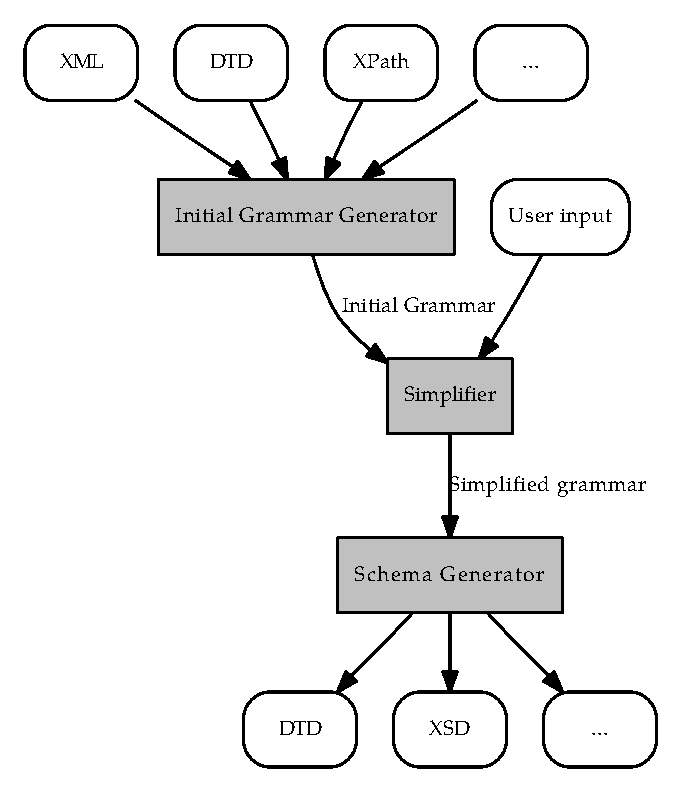
\includegraphics[width=0.5\textwidth]{images/inference-process}
\end{figure}

The responsibility of the first module, the \jmodule{Initial Grammar Generator}, is to parse all input files (documents, schemas and queries) and create a so-called \textit{initial grammar} (IG, TODO nomenclature). This is the representation in which will the structure live until it is used to create the final product - the schema. As the name suggests, IG is a grammar - an \textit{extended context-free grammar}, to be more precise (see \cite{extendedcfg}). As such, its left hand side is an element, its right hand side is a regular expression representing its content model. (TODO picture?) IG is used to create the AM model used in this thesis, too. jInfer contains one such module, the \jmodule{BasicIGG}, which is described in detail in \cite{basiciggdoc}.

After leaving the \jmodule{Initial Grammar Generator}, the IG needs to be made more general, shortened, \textit{simplified}. This is the responsibility of an aptly named module, the \jmodule{Simplifier}. To get the full idea about how this can be done it would be probably best to read Michal Klempa's thesis (TODO link), which describes this in great detail. Whatever happens, there is simplified grammar on the exit of \jmodule{Simplifier}, ready to be processed by...

The last module, \jmodule{Schema Generator} takes the simplified grammar and creates the resulting schema from it. This process is not too interesting, but anyone wishing to find out all about it is invited to read the documentation to the two \jmodule{Schema Generator}s bundled with jInfer - the BasicDTD and BasicXSD modules.

\chapter{\jmodule{IDSetSearch}}
\label{appendix-iss}

This appendix will shortly describe the \jmodule{IDSetSearch} jInfer module. As the name suggests, its main purpose is to find ID and IDREF sets and provide attribute statistics in general for grammars originating from any stage of XML schema inference. Virtually every piece of code that was added to jInfer in the course of creating this thesis is contained in this module.\\

From jInfer's point of view, this module resides in codebase \texttt{cz.\.cuni.\.mff.\.ksi.\.jinfer.\.iss} and is a service provider for \texttt{cz.\.cuni.\.mff.\.ksi.\.jinfer.\.base.\.inter\.faces.\.ID\.Set\.Search} interface. Invoking the \texttt{showIDSetPanel()} method displays a fully-featured window containing all the relevant attribute statistics as well as possibility to find the ID and IDREF sets for a specified grammar.\\

Most important packages in \jmodule{IDSetSearch} are the following.

\begin{itemize}
	\item \texttt{objects}, containing the object representation of attribute mappings and AM model.
	\item \texttt{heuristics.construction}, containing all the CHs hidden behind the \texttt{Con\-struc\-tion\-Heu\-ris\-tic} interface, with sub-packages \texttt{fidax} containing the whole implementation of FIDAX heuristic % TODO link
	and \texttt{glpk} containing the whole interface to an external GLPK solver. % TODO link
	\item \texttt{heuristics.improvement}, containing all the IH hidden behind the \texttt{Im\-prove\-ment\-Heu\-ris\-tic} interface.
	\item \texttt{experiments}, containing everything related to experimenting with these heuristics.
\end{itemize}

\texttt{Experiment} is a class representing a single experiment with specified input data (encapsulated in \texttt{Test\-Data} interface), settings (encapsulated in \texttt{Ex\-pe\-ri\-ment\-Pa\-ra\-me\-ters}) and a metaheuristic as defined in TODO link. Its method \texttt{run()} will launch the metaheuristic, first executing the construction heuristic and then running the specified improvement heuristics in a loop until termination criteria defined in an implementation of \texttt{Ter\-mi\-na\-tion\-Cri\-ter\-ion} are met. The quality of a single ID set is measured by an instance of \texttt{Quality\-Measurement}. After the experiment finishes, it invokes the \texttt{notify\-Finished()} method.\\

However, experiments are almost never run alone. For the purpose of running a whole experimental set there is the \texttt{Experiment\-Set} interface and its abstract implementation \texttt{Abstract\-Experiment\-Set}. Its descendants need only to provide a list of \texttt{Experiment\-Parameter}s and looping as well as data collection will be handled for them.

\section{How to Create a New Heuristic}

Decide whether it should be a CH or IH and create a class implementing \texttt{Con\-struc\-tion\-Heu\-ris\-tic} or \texttt{Im\-prove\-ment\-Heu\-ris\-tic}, respectively. In each case implement all the \texttt{get*Name()} methods inherited from \texttt{Named\-Module} and then the most important \texttt{start()} method.

In this method use the provided \texttt{Experiment} instance (and \texttt{List<IdSet> feasiblePool} in case of IH) to create a pool of feasible solutions and in the end return it by invoking the \texttt{finished()} method of the provided \texttt{Heuristic\-Callback} parameter.

\section{How to Create a New Experimental Set}

Subclass the \texttt{Abstract\-Experiment\-Set} class, override \texttt{get\-Name()} to provide the name of this set and finally override \texttt{get\-Experiments()} to return the list of \texttt{Experiment\-Parameters} that will constitute this sit.

It is possible to optionaly override any of the following methods: \texttt{notify\-Start()}, \texttt{notify\-Finished()} and \texttt{notify\-Finished\-All()}. They will be invoked before running the first experiment, after each experiment run and after all experiments finished, respectively. Note that \texttt{notify\-Finished()} already contains logic to output some information regarding the currently finished experiment to a file, but it can be safely overriden without a need to call \texttt{super.\.notify\-Finished()}.

\chapter{Experimental Trace}
\label{appendix-trace}

Following is a trace logged from a sample experiment run. It shows all the relevant information related to this instance, any and every piece of information we might be interested in.

To save space, 2-column layout is used. Commentary on the particulars follows right after its end.

\begin{multicols}{2}
\begin{scriptsize}
\begin{verbatim}
CPU info
  Intel(R) Core(TM)2 Quad CPU Q9550 @ 2.83GHz
  Cores: 4
  Clock speed: 2983 MHz
Memory info
  Size: 8192 MB
OS info
  Name: Windows 7
  Version: 6.1
  Architecture: amd64
Java info
  Version: 1.6.0_26
  VM: Java HotSpot(TM) 64-Bit Server VM
GLPK info
  GLPSOL: GLPK LP/MIP Solver 4.34

Configuration:
File name: graph.xml (101599 b)
  Graph representation: 82 vertices, 1101 edges
alpha: 1.0, beta: 1.0

Results:
Total time spent: 7754 ms
Final quality: 0.19951219512195123 (10 AMs)
Highest quality: 0.23463414634146343 (12 AMs)
Construction phase:
  Algorithm: Random
    Time taken: 248 ms / Time since start: 248 ms
    Pool size: 10
    Quality: 0.19975609756097568 (11 AMs)
Improvement phase:
  pass #1:
  Algorithm: RandomRemove, ratio = 0.2
    Time taken: 0 ms / Time since start: 841 ms
    Pool size: 10
    Quality: 0.15878048780487808 (9 AMs)
  pass #2:
  Algorithm: Mutation, ratio = 0.1, limit = 1 s
    Time taken: 1512 ms / Time since start: 2710 ms
    Pool size: 11
    Quality: 0.21975609756097558 (11 AMs)

  <... 7 more passes removed ...>

  pass #10:
  Algorithm: Remove Worst
    Time taken: 80 ms / Time since start: 7676 ms
    Pool size: 12
    Quality: 0.19951219512195123 (10 AMs)
Termination reason: Maximum iterations exceeded.

Time,Quality,AMs
248,0.19975609756097568,11
841,0.15878048780487808,9
2710,0.21975609756097558,11
2927,0.1890243902439024,9
4421,0.23463414634146343,12
4703,0.23463414634146343,12
4896,0.1960975609756098,10
5793,0.23463414634146337,12
5972,0.19951219512195123,10
7433,0.19951219512195123,10
7676,0.19951219512195123,10

ID
Element,Attribute,Weight
vertex0,attr,0.024146341463414635
vertex2,attr,0.01975609756097561
vertex33,attr,0.016829268292682928
vertex34,attr,0.02219512195121951
vertex4,attr,0.022682926829268292
vertex41,attr,0.014878048780487804
vertex7,attr,0.02170731707317073
vertex70,attr,0.018780487804878048
vertex76,attr,0.01780487804878049
vertex8,attr,0.02170731707317073
vertex80,attr,0.01780487804878049
vertex97,attr,0.016341463414634147

IDREF
Element,Attribute
\end{verbatim}
\end{scriptsize}
\end{multicols}

The first section deals with system information. Please note that some of these characteristics cannot be easily obtained programmatically and are thus stored in the source code as constants.\\
To obtain GLPK information, the program parses the first line of standard output produced by running \code{glpsol -v}. It tries to guess whether it's the Cygwin version by looking at the path to the binary.

The second section states the input file along with its size and graph representation (Section \ref{section-experiments-data}). Alpha and beta parameters for this instance belong here too.

\begin{footnotesize}
\begin{verbatim}
Configuration:
File name: graph.xml (101599 b)
  Graph representation: 82 vertices, 1101 edges
alpha: 1.0, beta: 1.0
\end{verbatim}
\end{footnotesize}

Results section opens stating the most important information first: how long did the experiment run and what was the highest and final quality (these two are potentially different). Numbers of attribute mappings in the best and final solution respectively are stated as well.

\begin{footnotesize}
\begin{verbatim}
Total time spent: 7754 ms
Final quality: 0.19951219512195123 (10 AMs)
Highest quality: 0.23463414634146343 (12 AMs)
\end{verbatim}
\end{footnotesize}

Construction phase results go next. Among reported information are the full identification of the heuristic (possibly along with its parameters), time taken, size of the pool created and the quality of the incumbent solution (again, with the number of its AMs).

\begin{footnotesize}
\begin{verbatim}
Algorithm: Random
  Time taken: 248 ms / Time since start: 248 ms
  Pool size: 10
  Quality: 0.19975609756097568 (11 AMs)
\end{verbatim}
\end{footnotesize}

Now for each of the improvement phases there is one section in output log. Information presented here has the same structure as with the construction phase. Please note that the \code{Pool size} is always measured \textit{after} the improvement run.

\begin{footnotesize}
\begin{verbatim}
Algorithm: Mutation, ratio = 0.1, limit = 1 s
  Time taken: 1512 ms / Time since start: 2710 ms
  Pool size: 11
  Quality: 0.21975609756097558 (11 AMs)
\end{verbatim}
\end{footnotesize}

After the last improvement phase, the reason why the metaheuristic terminated is stated. Possible causes are exceeding the maximum time available, maximum iterations or reaching the known optimum for this file and alpha / beta settings.
\\

To be able to reconstruct the progress of the metaheuristic, the next section contains CSV \nomenclature{CSV}{Comma Separated Values} formatted data for each iteration. Each row contains the time in milliseconds, quality of the incumbent solution and the number of its AMs.

\begin{footnotesize}
\begin{verbatim}
Time,Quality,AMs
...
841,0.15878048780487808,9
2710,0.21975609756097558,11
...
\end{verbatim}
\end{footnotesize}

And finally, it is important to know what is the ID/IDREF set recommended by this experiment run - the reason why we do all this! Thus the log is concluded by a CSV formatted list of element - attribute name pairs to be included in the ID and IDREF set, respectively.

\begin{footnotesize}
\begin{verbatim}
Element,Attribute,Weight
vertex0,attr,0.024146341463414635
...
\end{verbatim}
\end{footnotesize}

Note that in this example trace there were no \texttt{IDREF} AMs found. \qed

% TODO a QED square

\end{document}
